


\section{Principal Component Analysis}

\noindent From the PCA I obtain $12$ different principal components and their standard deviation. I have conducted PCA on the data from period $3$ as well as the whole dataset to compare. The PCA results from the whole dataset are shown in Table \ref{table:pca results} and the results from the Period $3$ data are shown Table \ref{table:pca results period 3}. They show the importance of each principal component. The results from period $3$ shows that the standard deviations are much larger for the first component, indicating then that the volatility is larger. The first principal component explains much more of the variation in the data from period 3 that it does for the whole dataset. The scree plot of the results from period $3$ is shown in Figure \ref{fig:scree plot period 3}, and it shows that two principal components seem to be sufficient. 

\begin{figure}[!htbp]
    \centering
    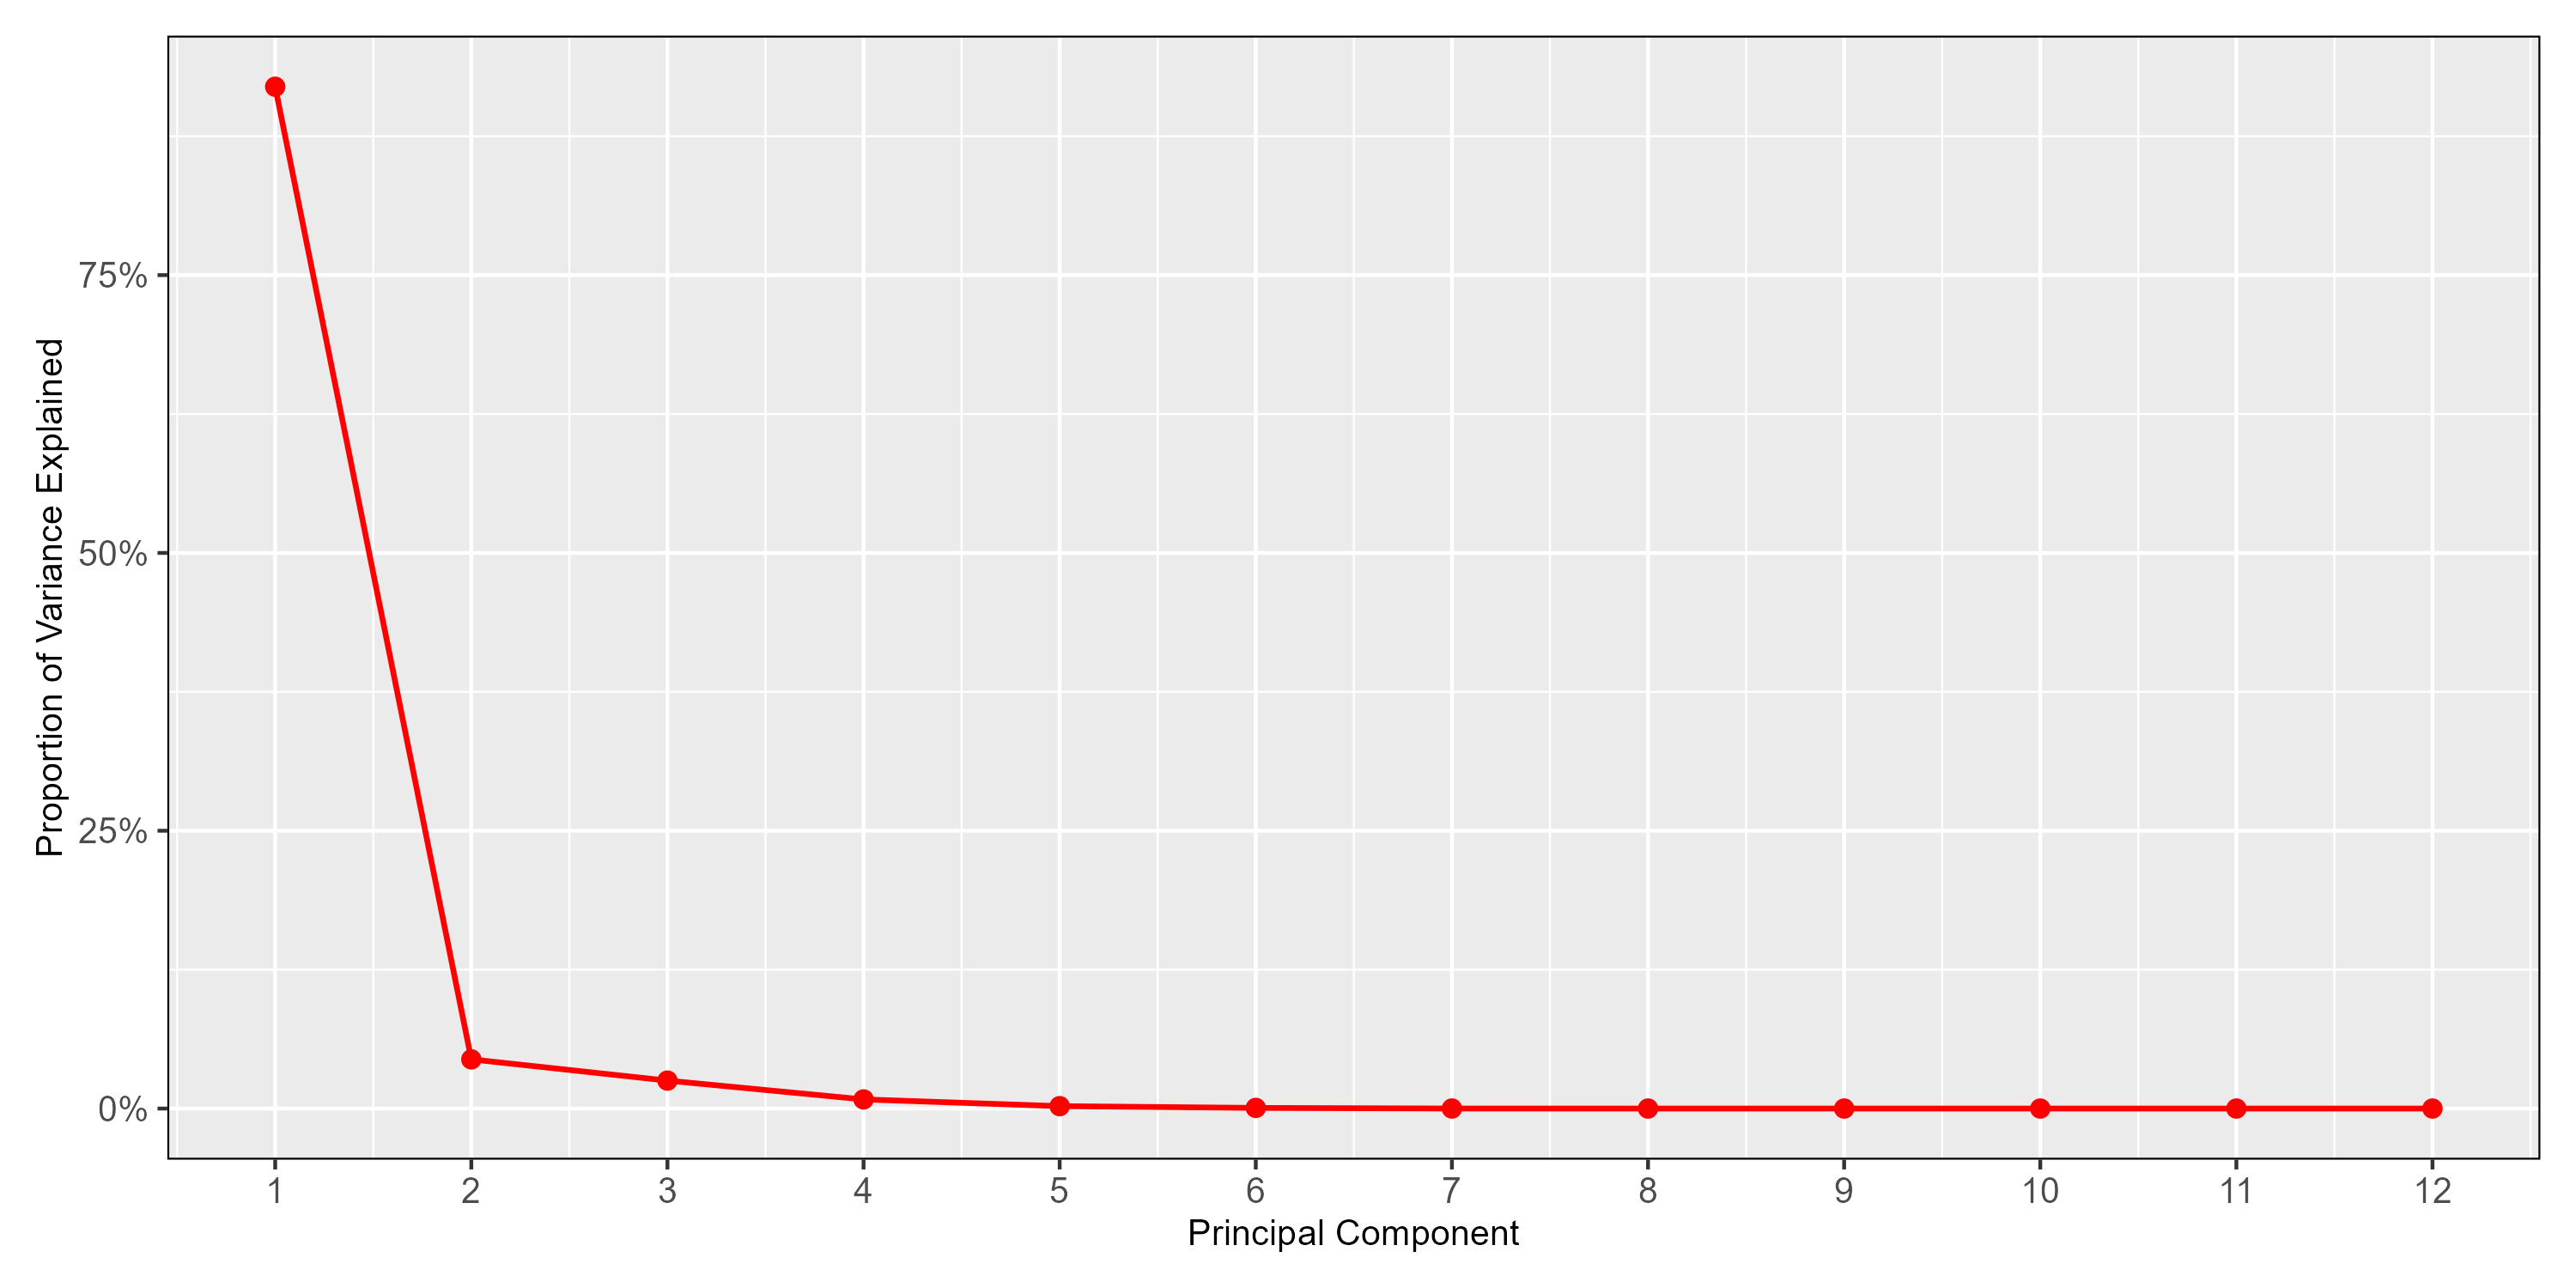
\includegraphics[width=.95\linewidth]{Figures/Scree Plot/zero_coupon_yields_phase_3_scree_plot.png}
    \caption[Scree plot, Period 3.]{Scree plot, Period 3. Two principal components seem to be sufficient.}
    \label{fig:scree plot period 3}
\end{figure}

\newpage

\begin{table}[!htbp]
\centering
\begin{tabular}{|m{9em}|c|c|c|c|c|} 
\cline{2-6}
\multicolumn{1}{c|}{} & PC1 & PC2 & PC3 & PC4 & $\cdots$ \\ \hline
Standard deviation & $0.01936$ & $0.00605$ & $0.00341$ & $0.00189$ & $\cdots$ \\ \hline
Proportion of Variance Explained & $0.87594$ & $0.08539$ & $0.02715$ & $0.00831$ & $\cdots$ \\
\hline
Cumulative Proportion of Variance Explained & $0.87594$ & $0.96133$ & $0.98848$ & $0.99679$ & $\cdots$ \\
\hline
\end{tabular}
\caption[PCA results]{PCA results.}
\label{table:pca results}
\end{table}

\begin{table}[!htbp]
\centering
\begin{tabular}{|m{9em}|c|c|c|c|c|} 
\cline{2-6}
\multicolumn{1}{c|}{} & PC1 & PC2 & PC3 & PC4 & $\cdots$ \\ \hline
Standard deviation & $0.02415$ & $0.00530$ & $0.00400$ & $0.00229$ & $\cdots$ \\ \hline
Proportion of Variance Explained & $0.91951$ & $0.04427$ & $0.02516$ & $0.00823$ & $\cdots$ \\
\hline
Cumulative Proportion of Variance Explained & $0.91951$ & $0.96378$ & $0.98895$ & $0.99718$ & $\cdots$ \\
\hline
\end{tabular}
\caption[PCA results, Period 3.]{PCA results, Period 3.}
\label{table:pca results period 3}
\end{table}



\section{Volatilities}

\subsection{Observed Volatilities}

\noindent From the PCA on the whole dataset I get the corresponding volatilities for the two factors, and they are shown in Figure \ref{fig:observed volatilites}. The observed volatilities from the period $3$ data are shown in Figure \ref{fig:observed volatilites period 3}. These figures shows that the volatilities from period 3 are much larger than the volatilities from the whole dataset, but the volatility structures are almost identical. For period 3, we can see that the volatility is higher for larger tenors, and smaller for short tenors.

\subsection{Fitted Volatilities}

\noindent The fitted volatilities obtained from period 3 for all four models are shown in Figure \ref{fig:fitted volatilites period 3}. This figure shows the difference between the cubic polynomial regression and the natural cubic spline regression. For the first factor, the spline fits the data more accurately, with a curve at the short tenors and with a straight line at the larger tenors. The cubic polynomial is really curved at the larger tenors. The fitted volatility for the second factor however is identical for all four models.

\vfill


\vfill

\begin{figure}[!htbp]
    \centering
    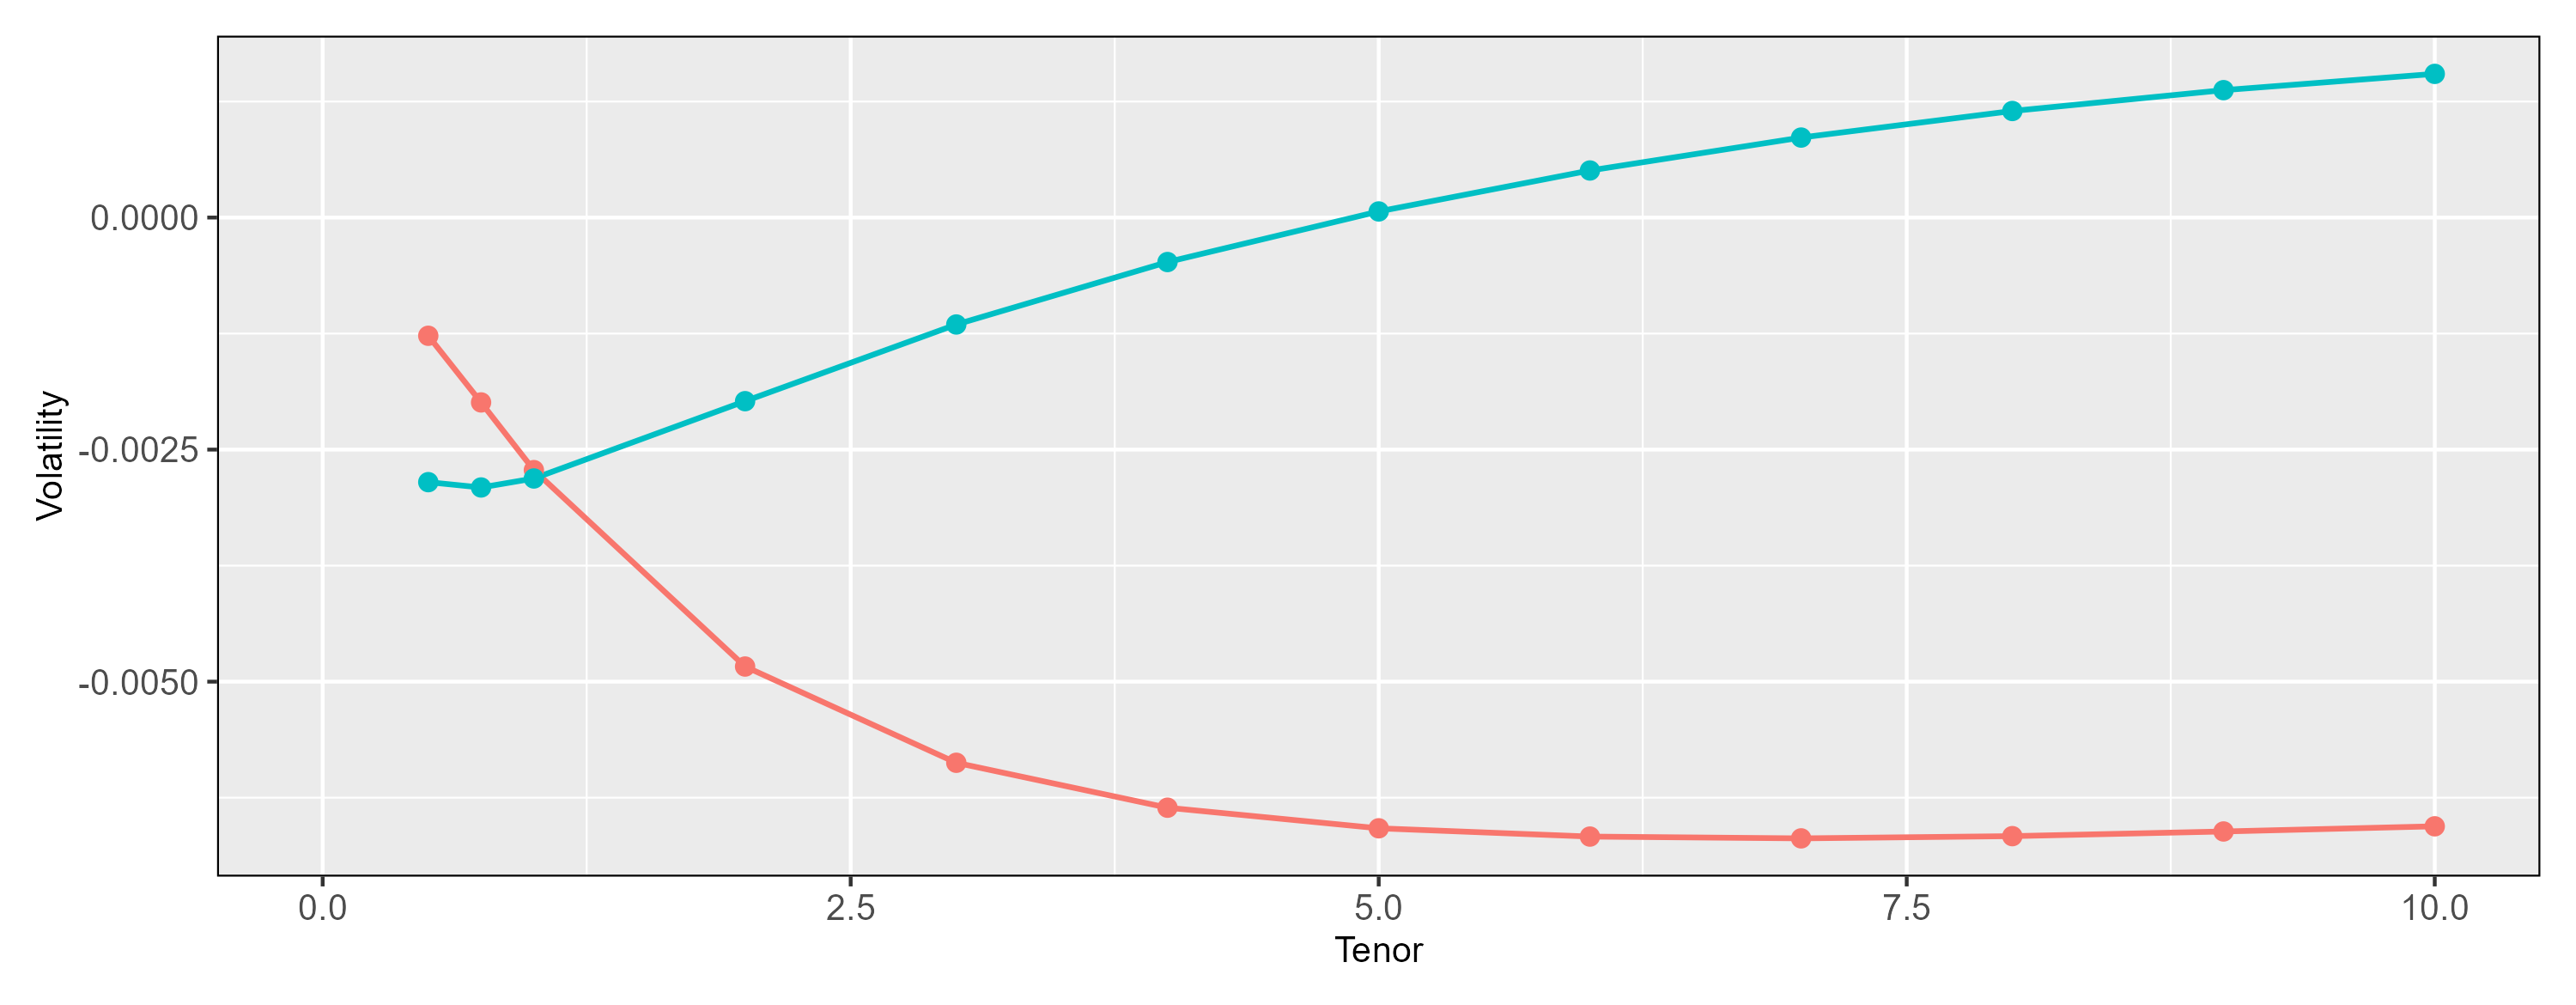
\includegraphics[width=.95\linewidth]{Figures/Volatilities/zero_coupon_yields_small_volatilities_plot.png}
    
    \caption[Observed Volatilities for the two factors]{Observed Volatilities for the two factors. The \textbf{rose} $\bigl($\textcolor{rose_}{\textbf{---}}$\bigr)$ colored line shows the volatility for the first factor. The \textbf{dark teal} $\bigl($\textcolor{dark_teal_}{\textbf{---}}$\bigr)$ colored line shows the volatility for the second factor.}
    \label{fig:observed volatilites}
\end{figure}

\vfill

\begin{figure}[!htbp]
    \centering
    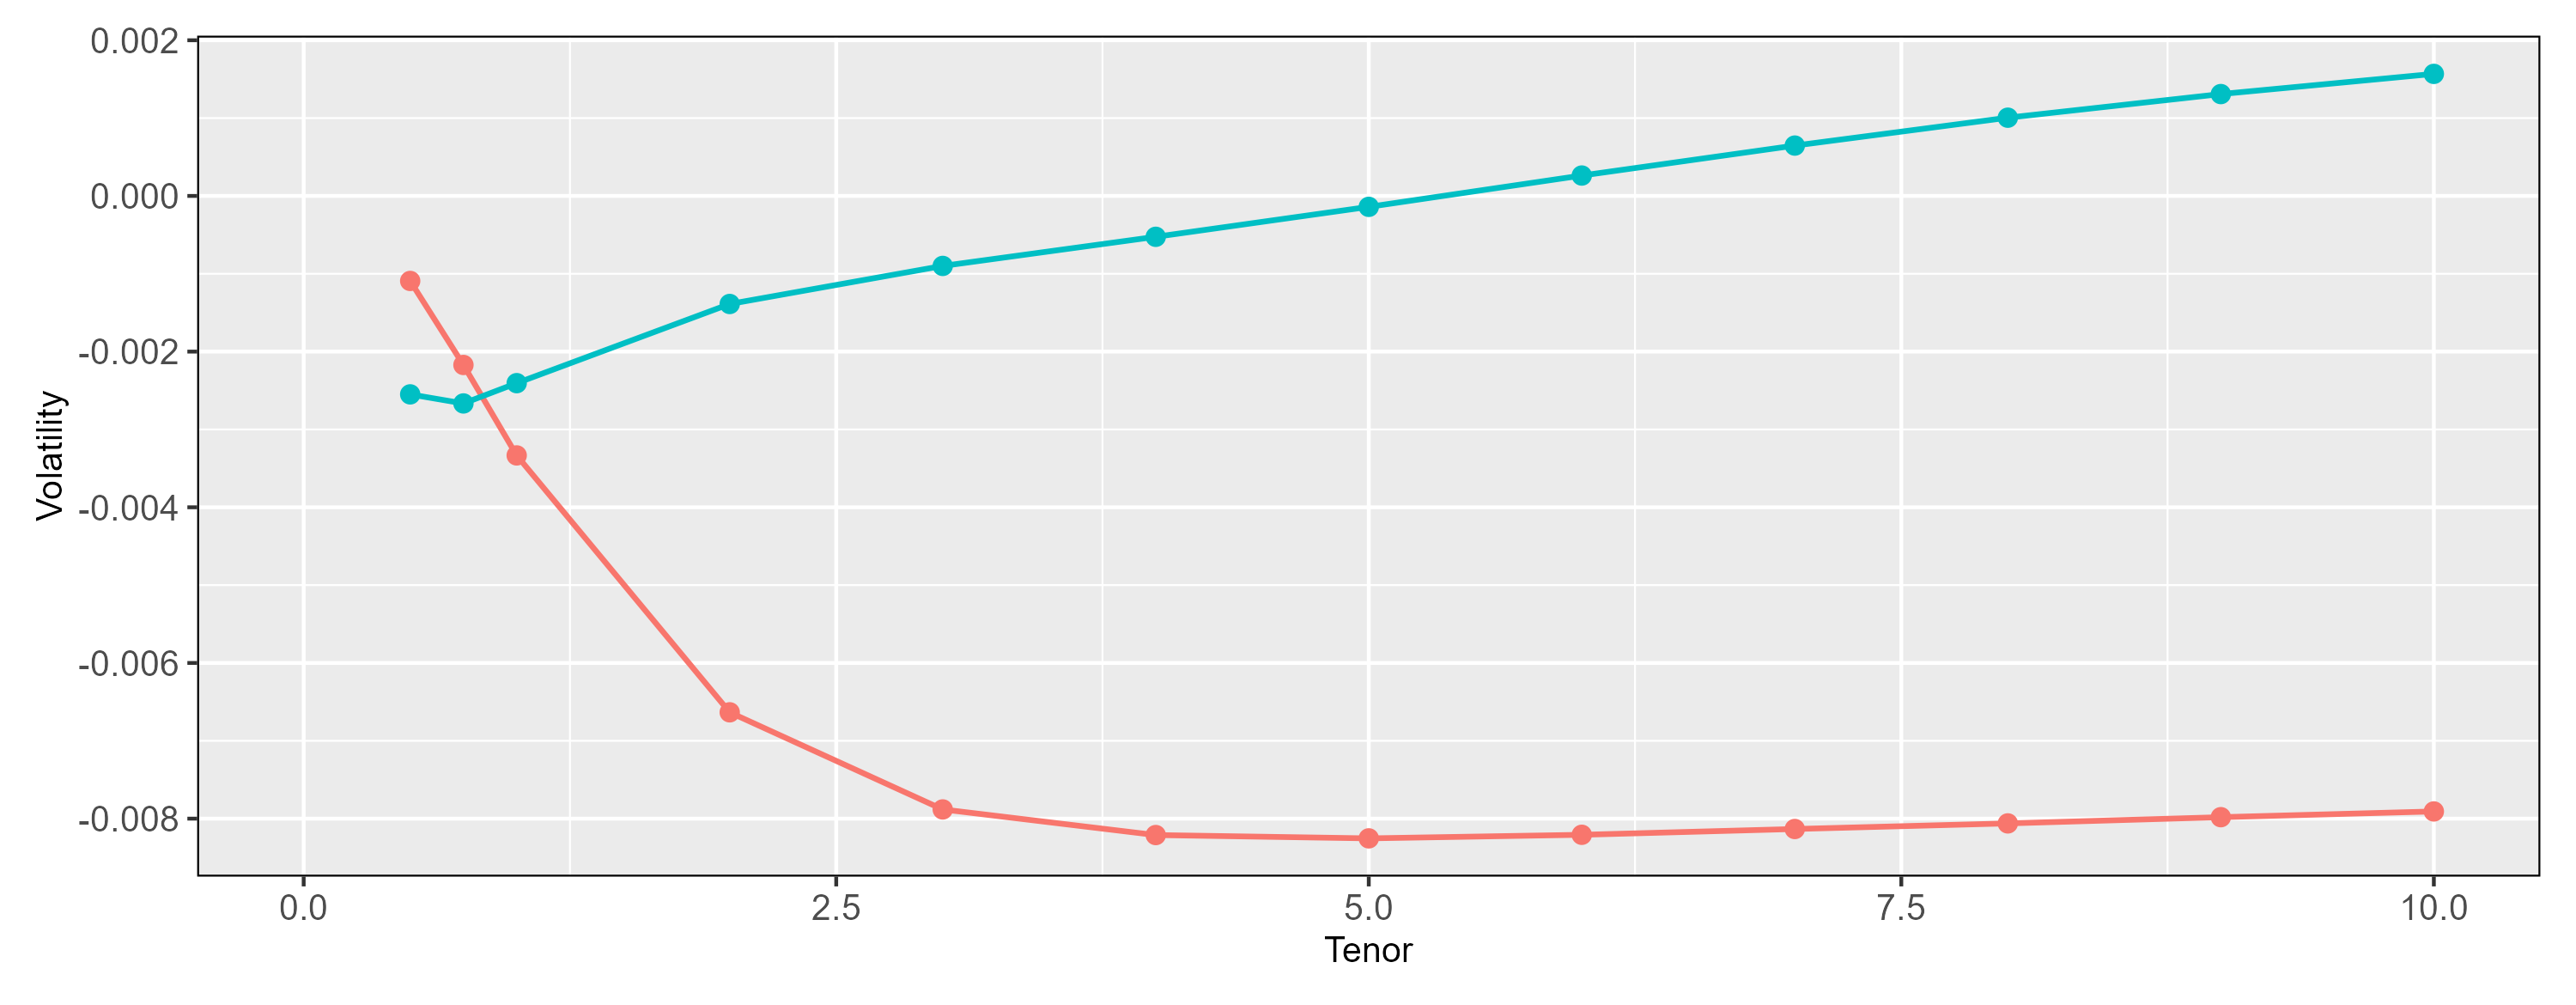
\includegraphics[width=.95\linewidth]{Figures/Volatilities/zero_coupon_yields_phase_3_small_volatilities_plot.png}
    
    \caption[Observed Volatilities for the two factors, Period 3]{Observed Volatilities for the two factors, Period 3. The \textbf{rose} $\bigl($\textcolor{rose_}{\textbf{---}}$\bigr)$ colored line shows the volatility for the first factor. The \textbf{dark teal} $\bigl($\textcolor{dark_teal_}{\textbf{---}}$\bigr)$ colored line shows the volatility for the second factor.}
    \label{fig:observed volatilites period 3}
\end{figure}

\vfill

\begin{figure}[!htbp]
    \centering
    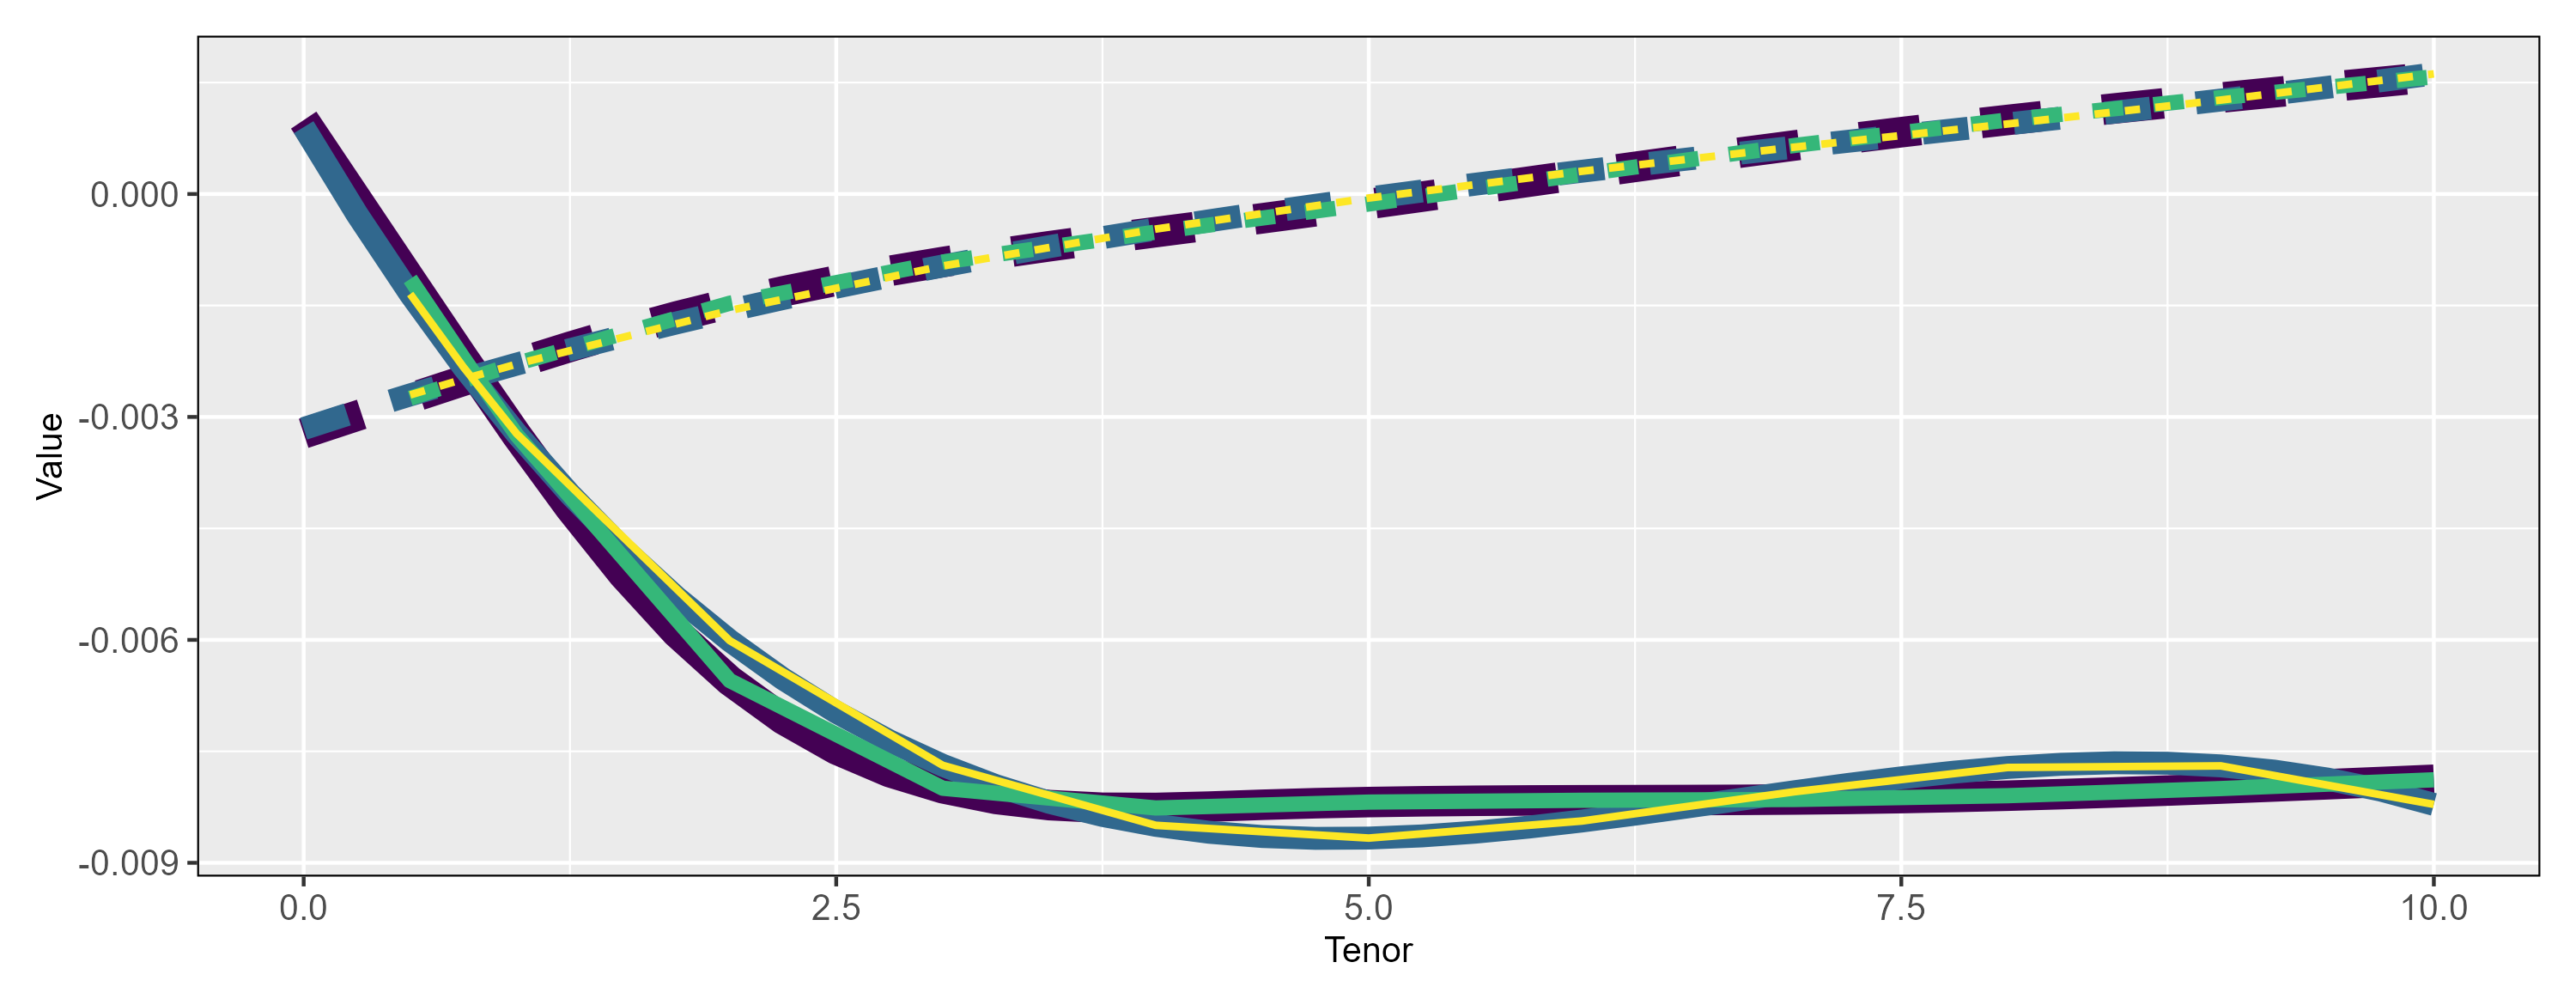
\includegraphics[width=.95\linewidth]{Figures/Fitted Volatilities/zero_coupon_yields_phase_3_HJM_2F_small_fitted_volatilities_plot.png}
    
    \caption[Fitted Volatilities for the two factors, Period 3]{Fitted Volatilities for the two factors, Period 3. The solid lines are the fitted volatilities for the first factor, and the dashed lines are the fitted volatilities for the second factor. The \textbf{yellow} $\bigl($\textcolor{yellow_}{\textbf{---}}$\bigr)$ and \textbf{green} $\bigl($\textcolor{green_}{\textbf{---}}$\bigr)$ colored lines are obtained from procedure $1$ and fitted using cubic polynomials and natural cubic splines respectively. The \textbf{dark blue} $\bigl($\textcolor{dark_blue_1}{\textbf{---}}$\bigr)$ and \textbf{dark purple} $\bigl($\textcolor{dark_purple_}{\textbf{---}}$\bigr)$ colored lines are obtained from procedure $2$ and fitted using cubic polynomials and natural cubic splines respectively.}
    \label{fig:fitted volatilites period 3}
\end{figure}

\vfill


\newpage

\section{Drifts}

\noindent The drift is the first term in Equation \eqref{eq:hjm fit model}, and the drifts obtained from all four models are shown in Figure \ref{fig:drifts period 3}. We see that the cubic polynomial regression gives a more curved result. At long tenors, we have lower drifts when compared to the spline models, which are more stable. 

\begin{figure}[!htbp]
    \centering
    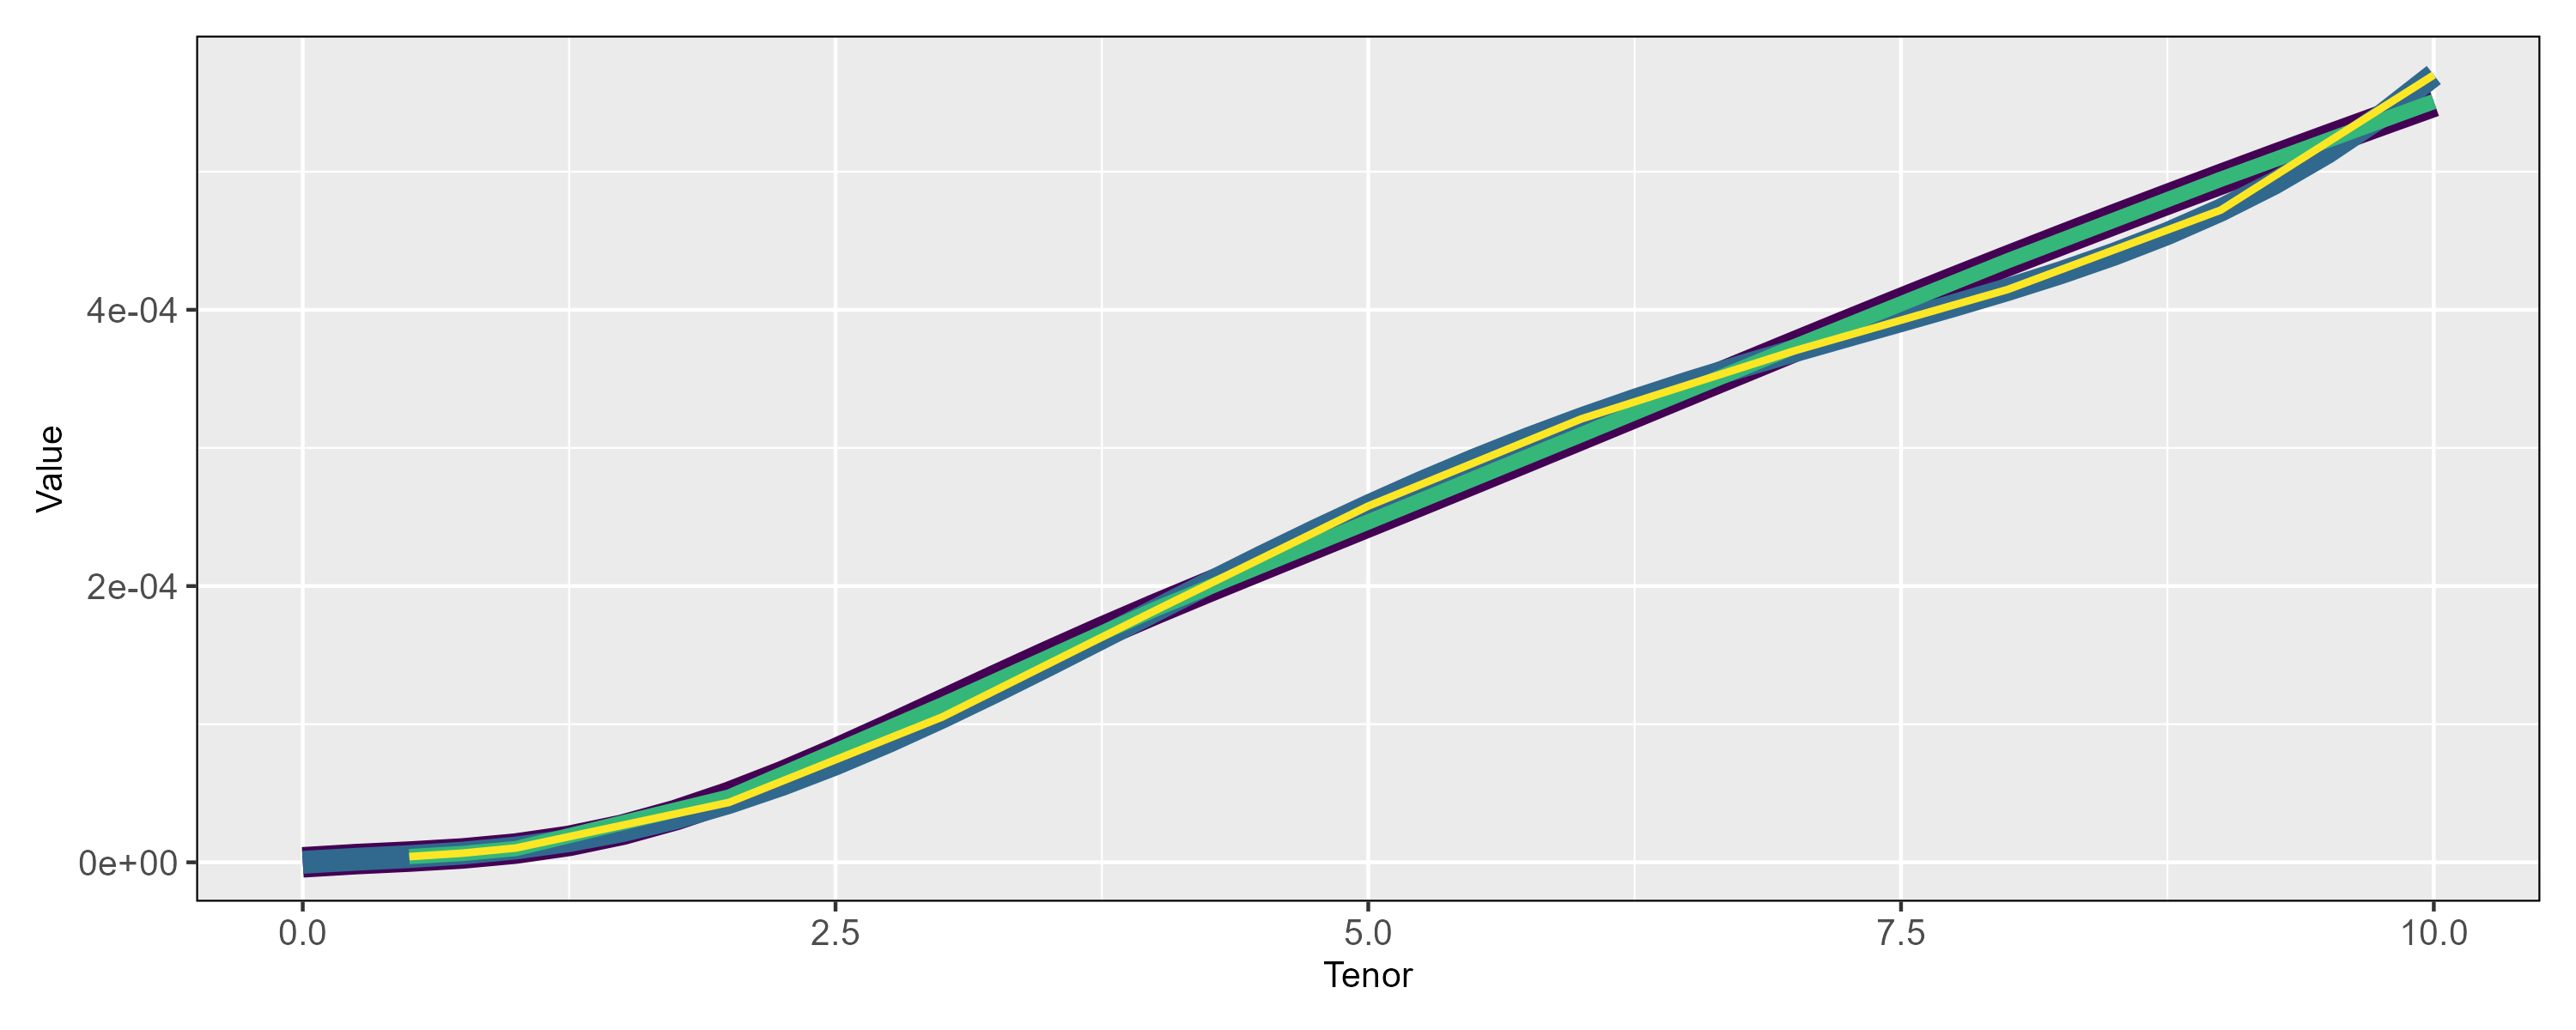
\includegraphics[width=.95\linewidth]{Figures/Drifts/zero_coupon_yields_phase_3_HJM_2F_small_drifts_plot.png}
    
    \caption[Drifts, period 3]{Drifts, period 3. The \textbf{yellow} $\bigl($\textcolor{yellow_}{\textbf{---}}$\bigr)$ and \textbf{green} $\bigl($\textcolor{green_}{\textbf{---}}$\bigr)$ colored lines are obtained from procedure $1$ and fitted using a cubic polynomial and a natural cubic spline respectively. The \textbf{dark blue} $\bigl($\textcolor{dark_blue_1}{\textbf{---}}$\bigr)$ and \textbf{dark purple} $\bigl($\textcolor{dark_purple_}{\textbf{---}}$\bigr)$ colored lines are obtained from procedure $2$ and fitted using a cubic polynomial and a natural cubic spline respectively.}
    \label{fig:drifts period 3}
\end{figure}



\section{Model Evaluation}

\noindent Figure \ref{fig:resid vs fit p 1} shows the residual vs. fits plots from procedure 1. There is no pattern for the tenors. Figure \ref{fig:resid vs fit p 2} in the appendix shows the residual vs. fits plots from procedure 2. These results show that procedure 2 have a few outliers. At large fitted values, the variance assumption seem not to hold for both the polynomial and the spline models.

Figure \ref{fig:qq p 1} shows the Q-Q plots from procedure 1. For the $2$-year, $6$-year, and $10$-year tenors the normality assumption holds exactly, but for the other tenors the data has heavier tails that the model fails to predict. This is true for both the polynomial and spline models. Figure \ref{fig:qq p 2} in the appendix shows the Q-Q plots from procedure 1. The normality assumption seem to hold for all tenors.

In Figure \ref{fig:Error}, I have plotted the LGOCV errors for my models based on period 3. We can see that the different procedures have large differences at short tenors.



\begin{figure}[!htbp]
    \centering
    \captionsetup{type=figure}
    \begin{subfigure}{0.49\textwidth}
        \centering
        \captionsetup{justification=centering}
        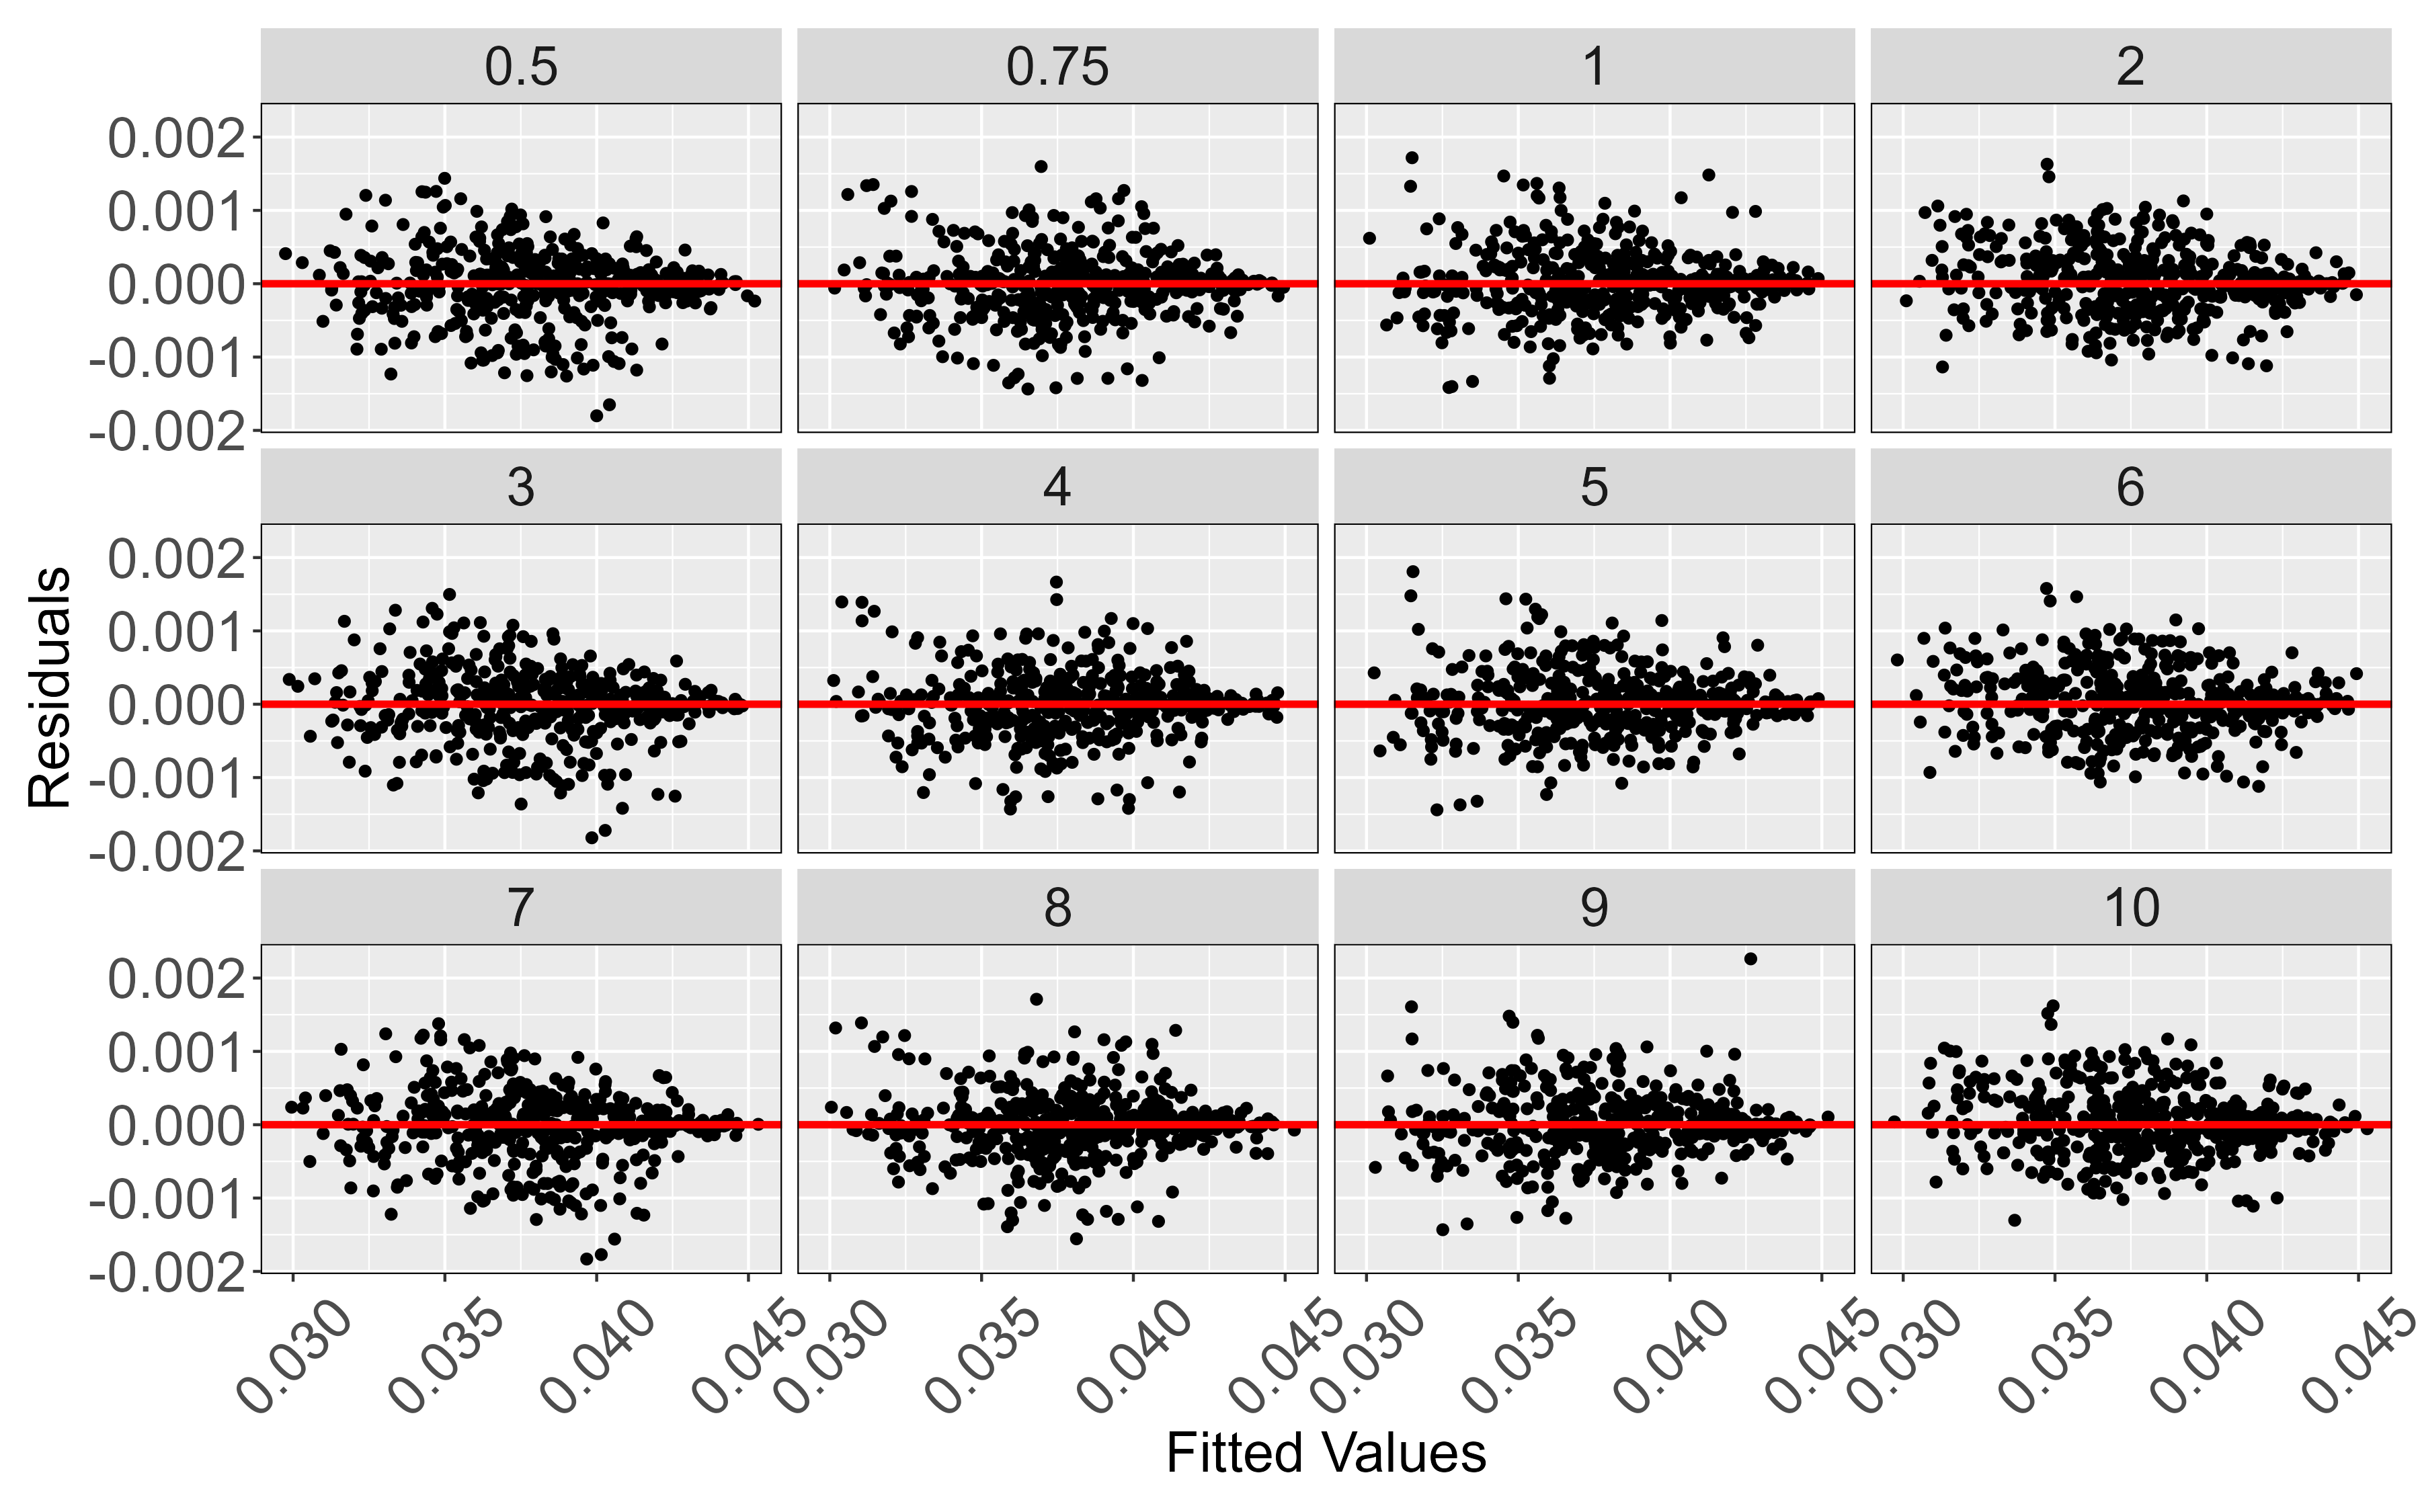
\includegraphics[width=\textwidth]{Figures/Model Checking/zero_coupon_yields_phase_3_HJM_2F_procedure_1_poly_model_fitted_vs_residual_plot.png}
        \subcaption{Volatilities fitted using polynomials.}
        \label{fig:resid vs fit poly model p 1}
    \end{subfigure}
    \hfill
    \begin{subfigure}{0.49\textwidth}
        \centering
        \captionsetup{justification=centering}
        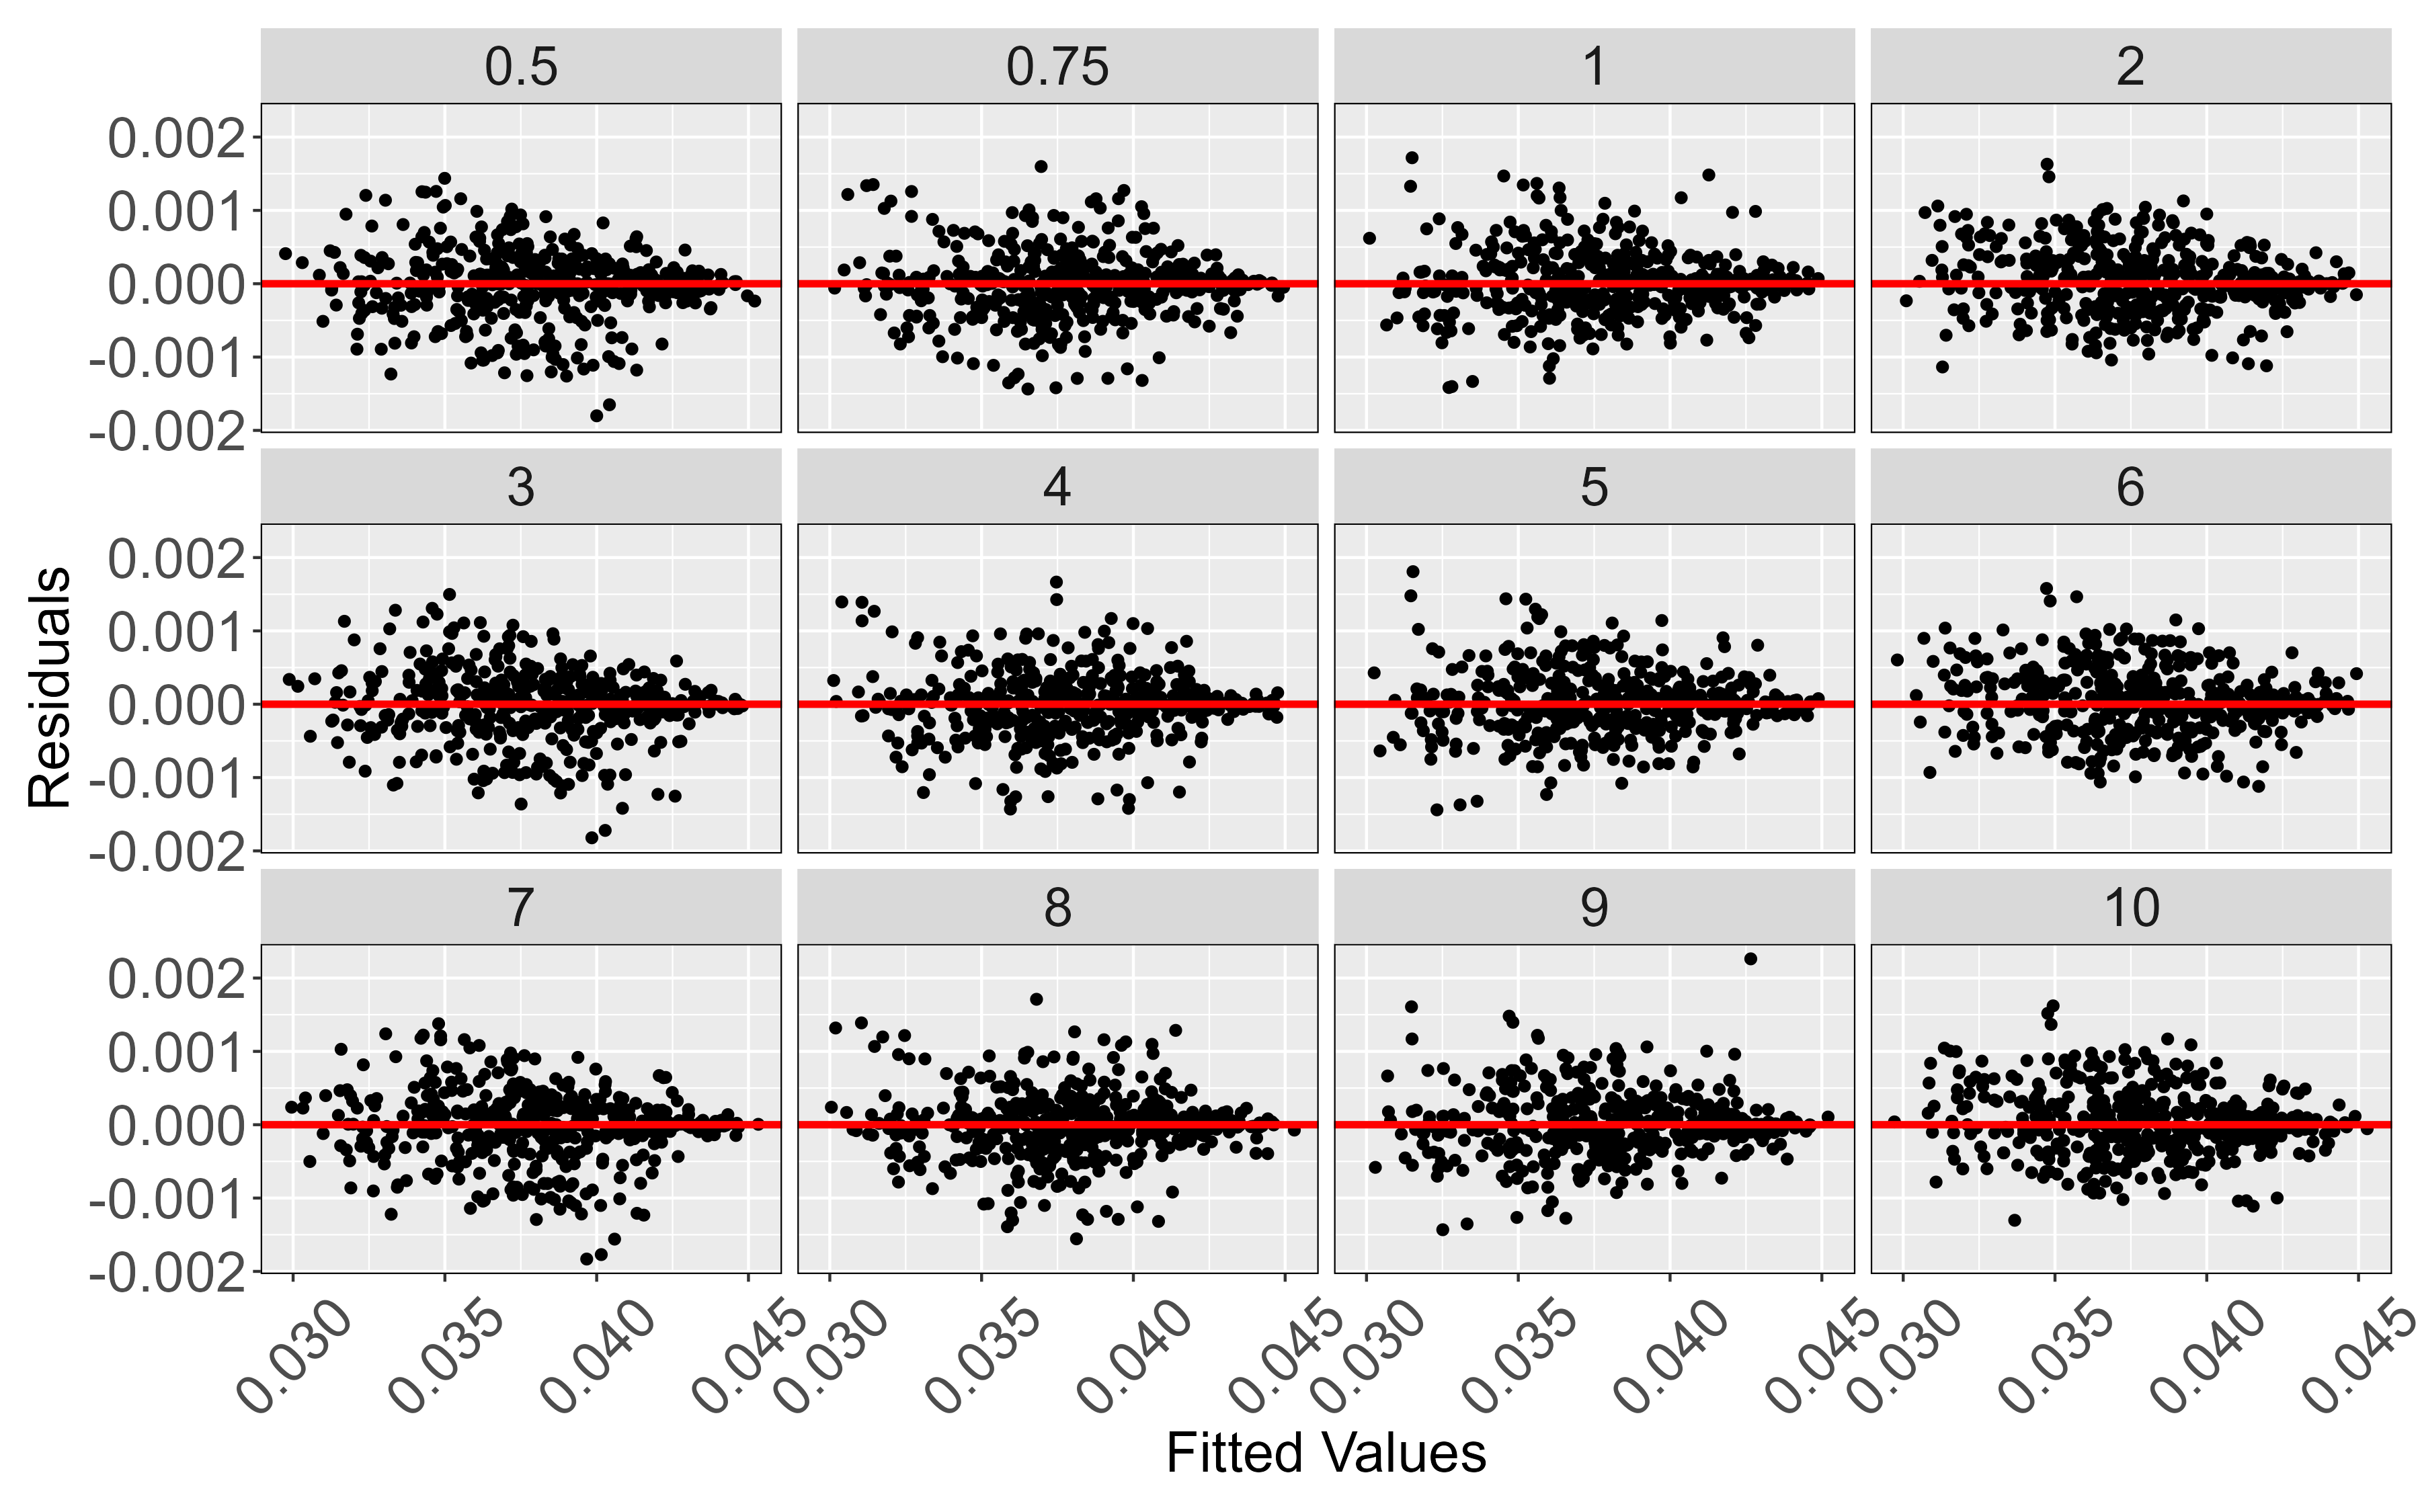
\includegraphics[width=\textwidth]{Figures/Model Checking/zero_coupon_yields_phase_3_HJM_2F_procedure_1_spline_model_fitted_vs_residual_plot.png}
        \subcaption{Volatilities fitted using splines.}
        \label{fig:resid vs fit spline model p 1}
    \end{subfigure}
    \caption[The Residuals vs. Fits Plots for the models using Procedure 1 for all tenors.]{The Residuals vs. Fits Plots for the models using Procedure 1 for all tenors. They show that there is equal variance across all fitted values. This means that the model assumption of equal variance across all dates is correct.}
    \label{fig:resid vs fit p 1}
\end{figure}

\begin{figure}[!htbp]
    \centering
    \captionsetup{type=figure}
    \begin{subfigure}{0.49\textwidth}
        \centering
        \captionsetup{justification=centering}
        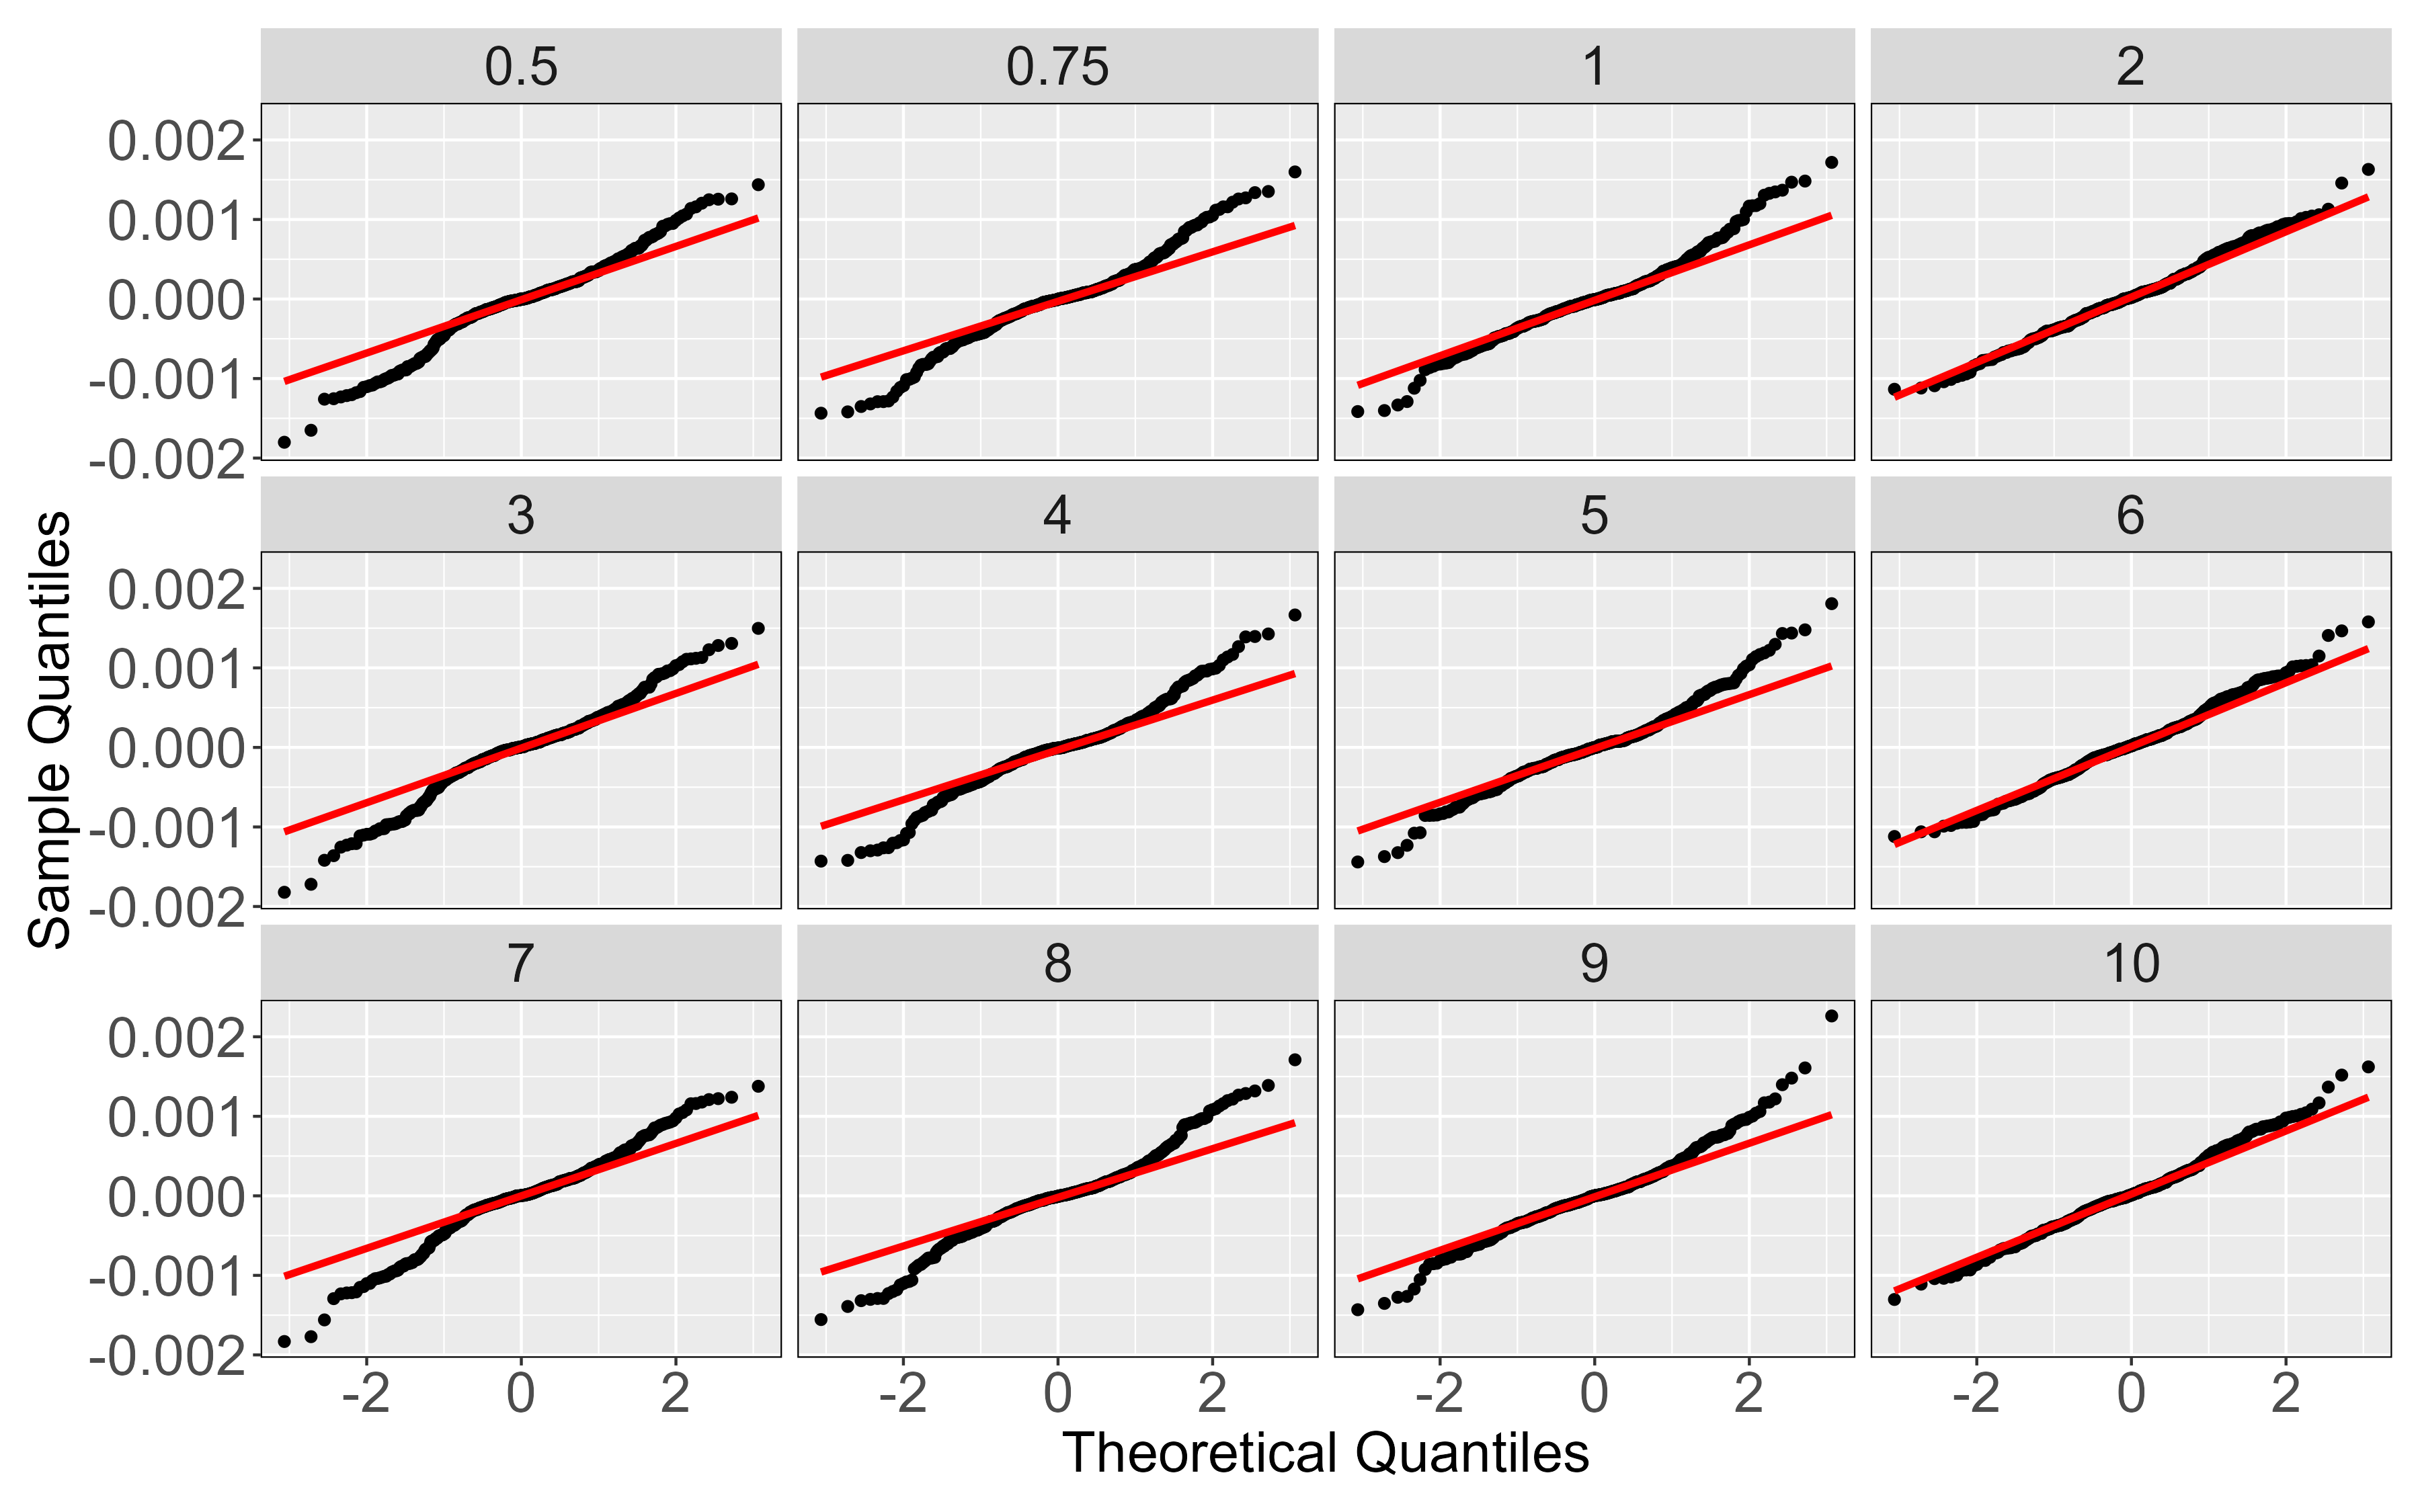
\includegraphics[width=\textwidth]{Figures/Model Checking/zero_coupon_yields_phase_3_HJM_2F_procedure_1_poly_model_qq_plot.png}
        \subcaption{Volatilities fitted using polynomials.}
        \label{fig:qq poly model p 1}
    \end{subfigure}
    \hfill
    \begin{subfigure}{0.49\textwidth}
        \centering
        \captionsetup{justification=centering}
        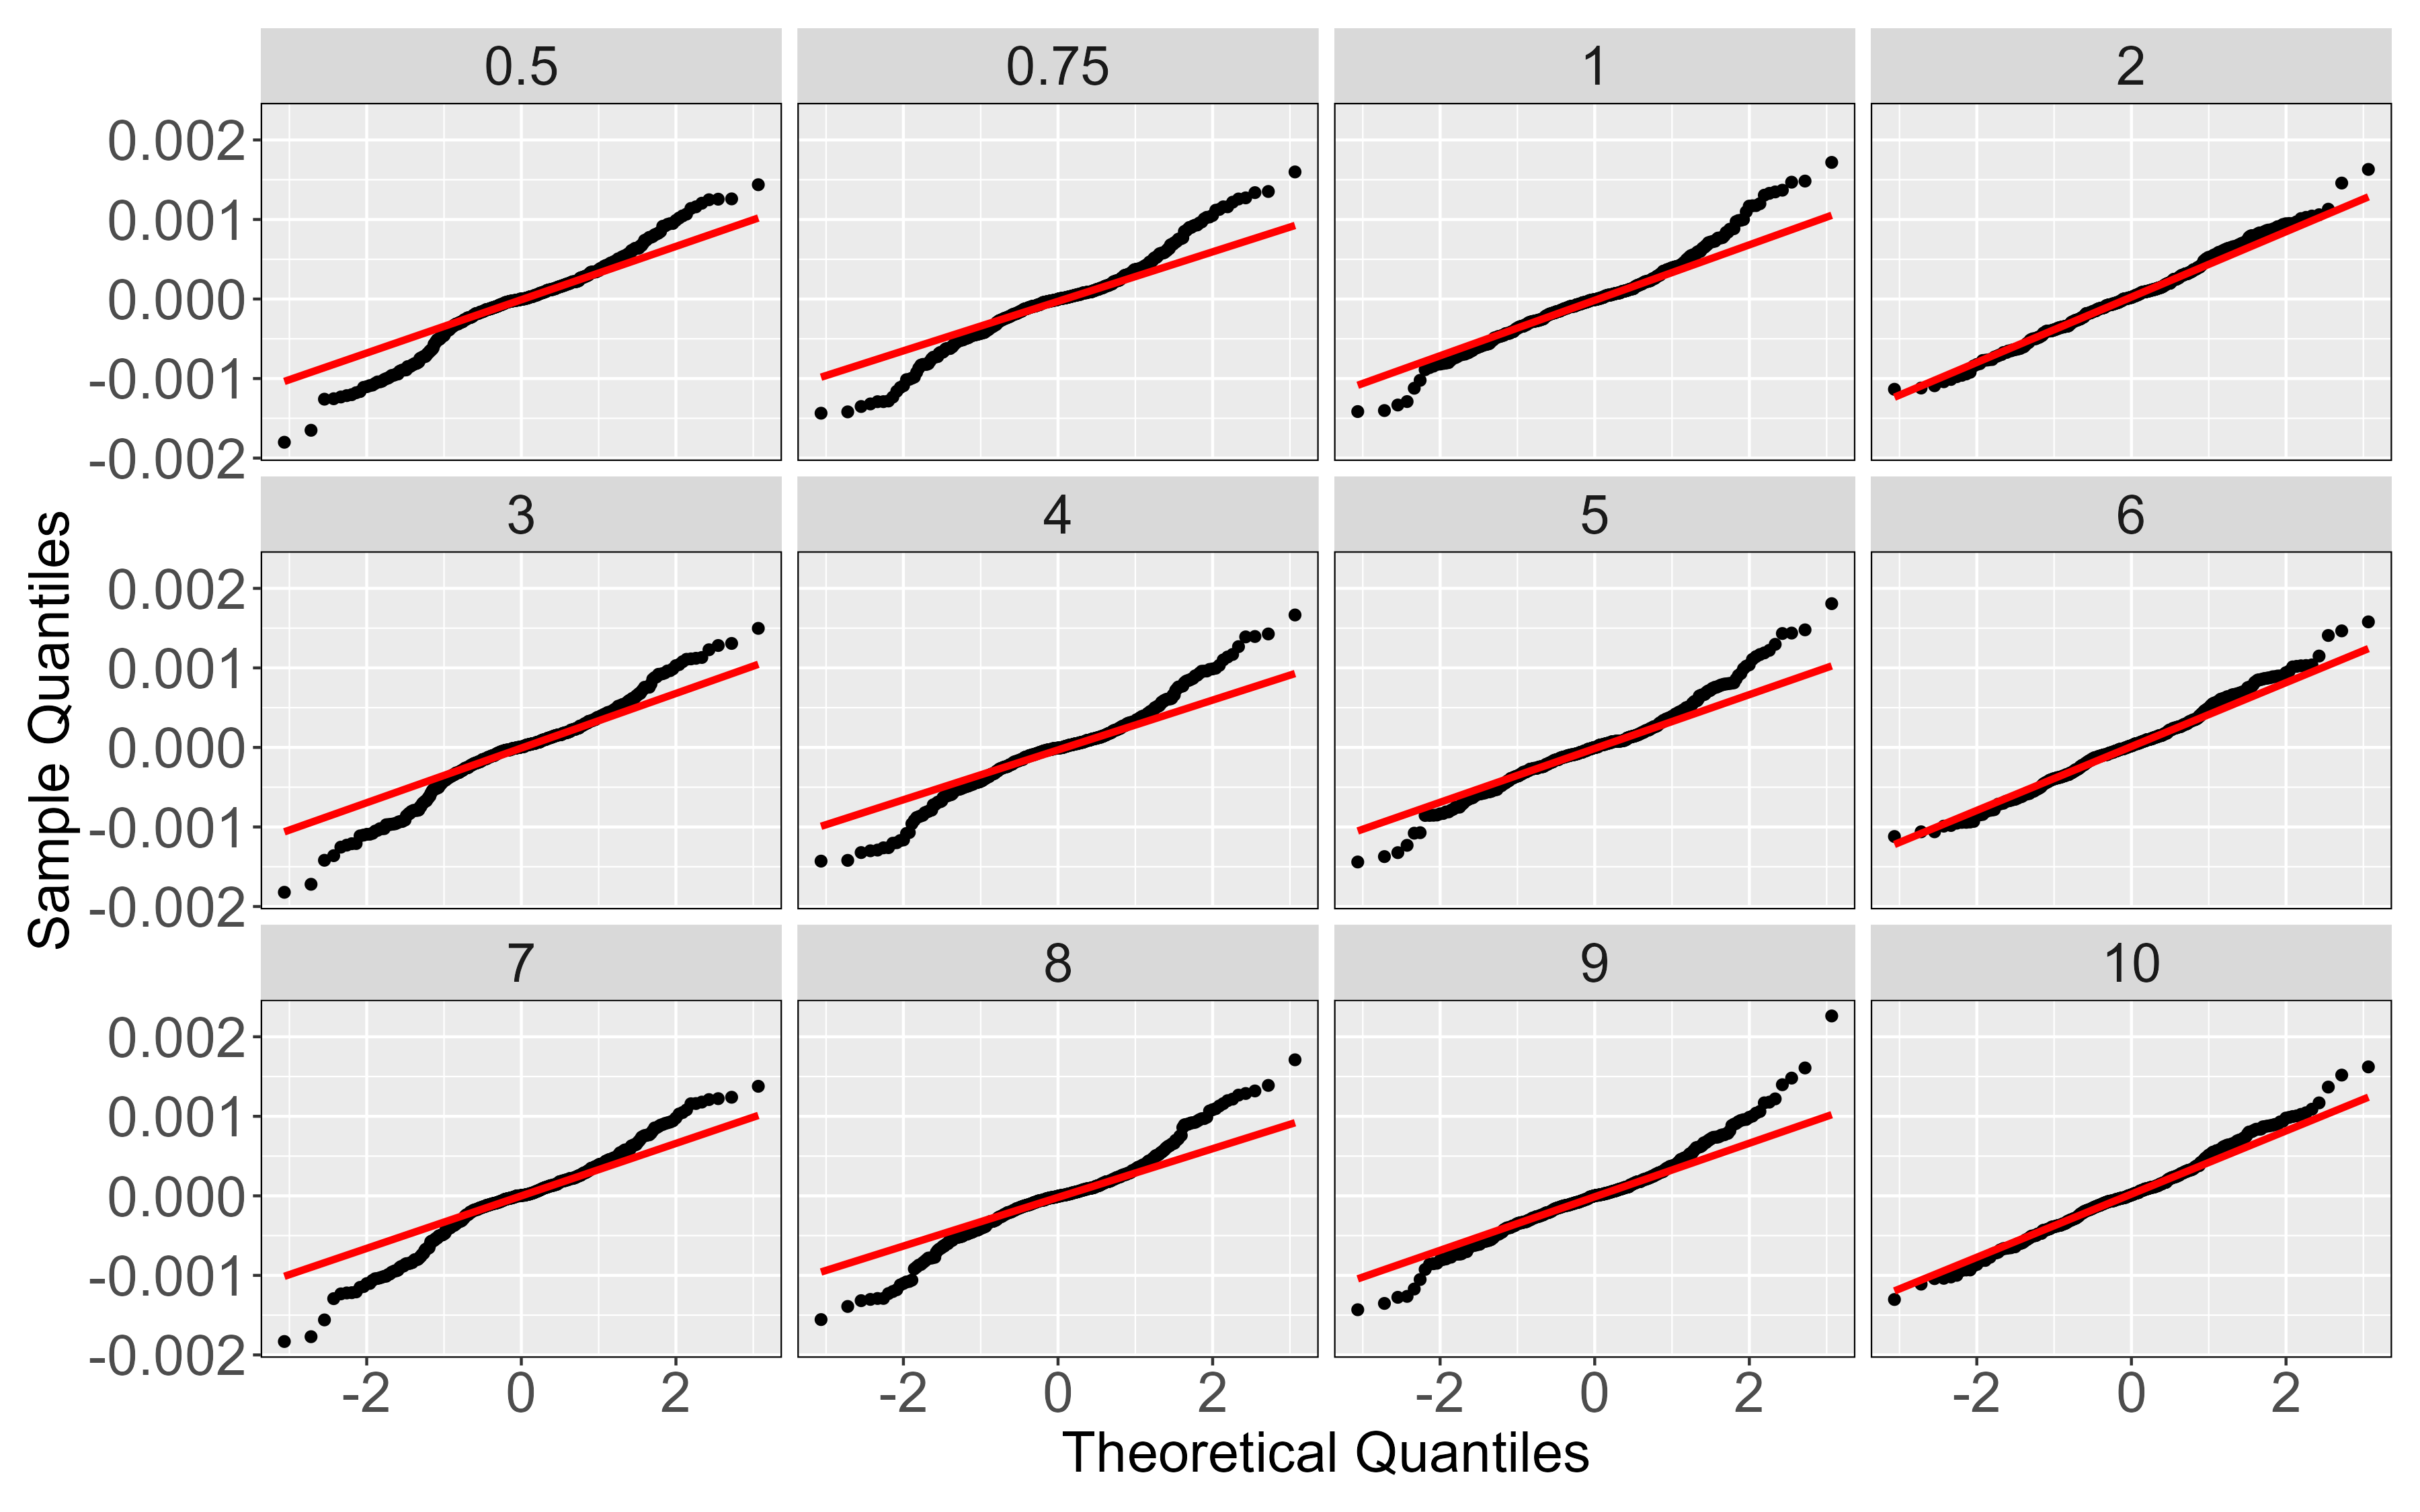
\includegraphics[width=\textwidth]{Figures/Model Checking/zero_coupon_yields_phase_3_HJM_2F_procedure_1_spline_model_qq_plot.png}
        \subcaption{Volatilities fitted using splines.}
        \label{fig:qq spline model p 1}
    \end{subfigure}
    \caption[The QQ-Plots for the models using Procedure 1 for all tenors.]{The QQ-Plots for the models using Procedure 1 for all tenors. They show that the real data has heavier tails than what the models can predict.}
    \label{fig:qq p 1}
\end{figure}

\begin{figure}[!htbp]
    \centering
    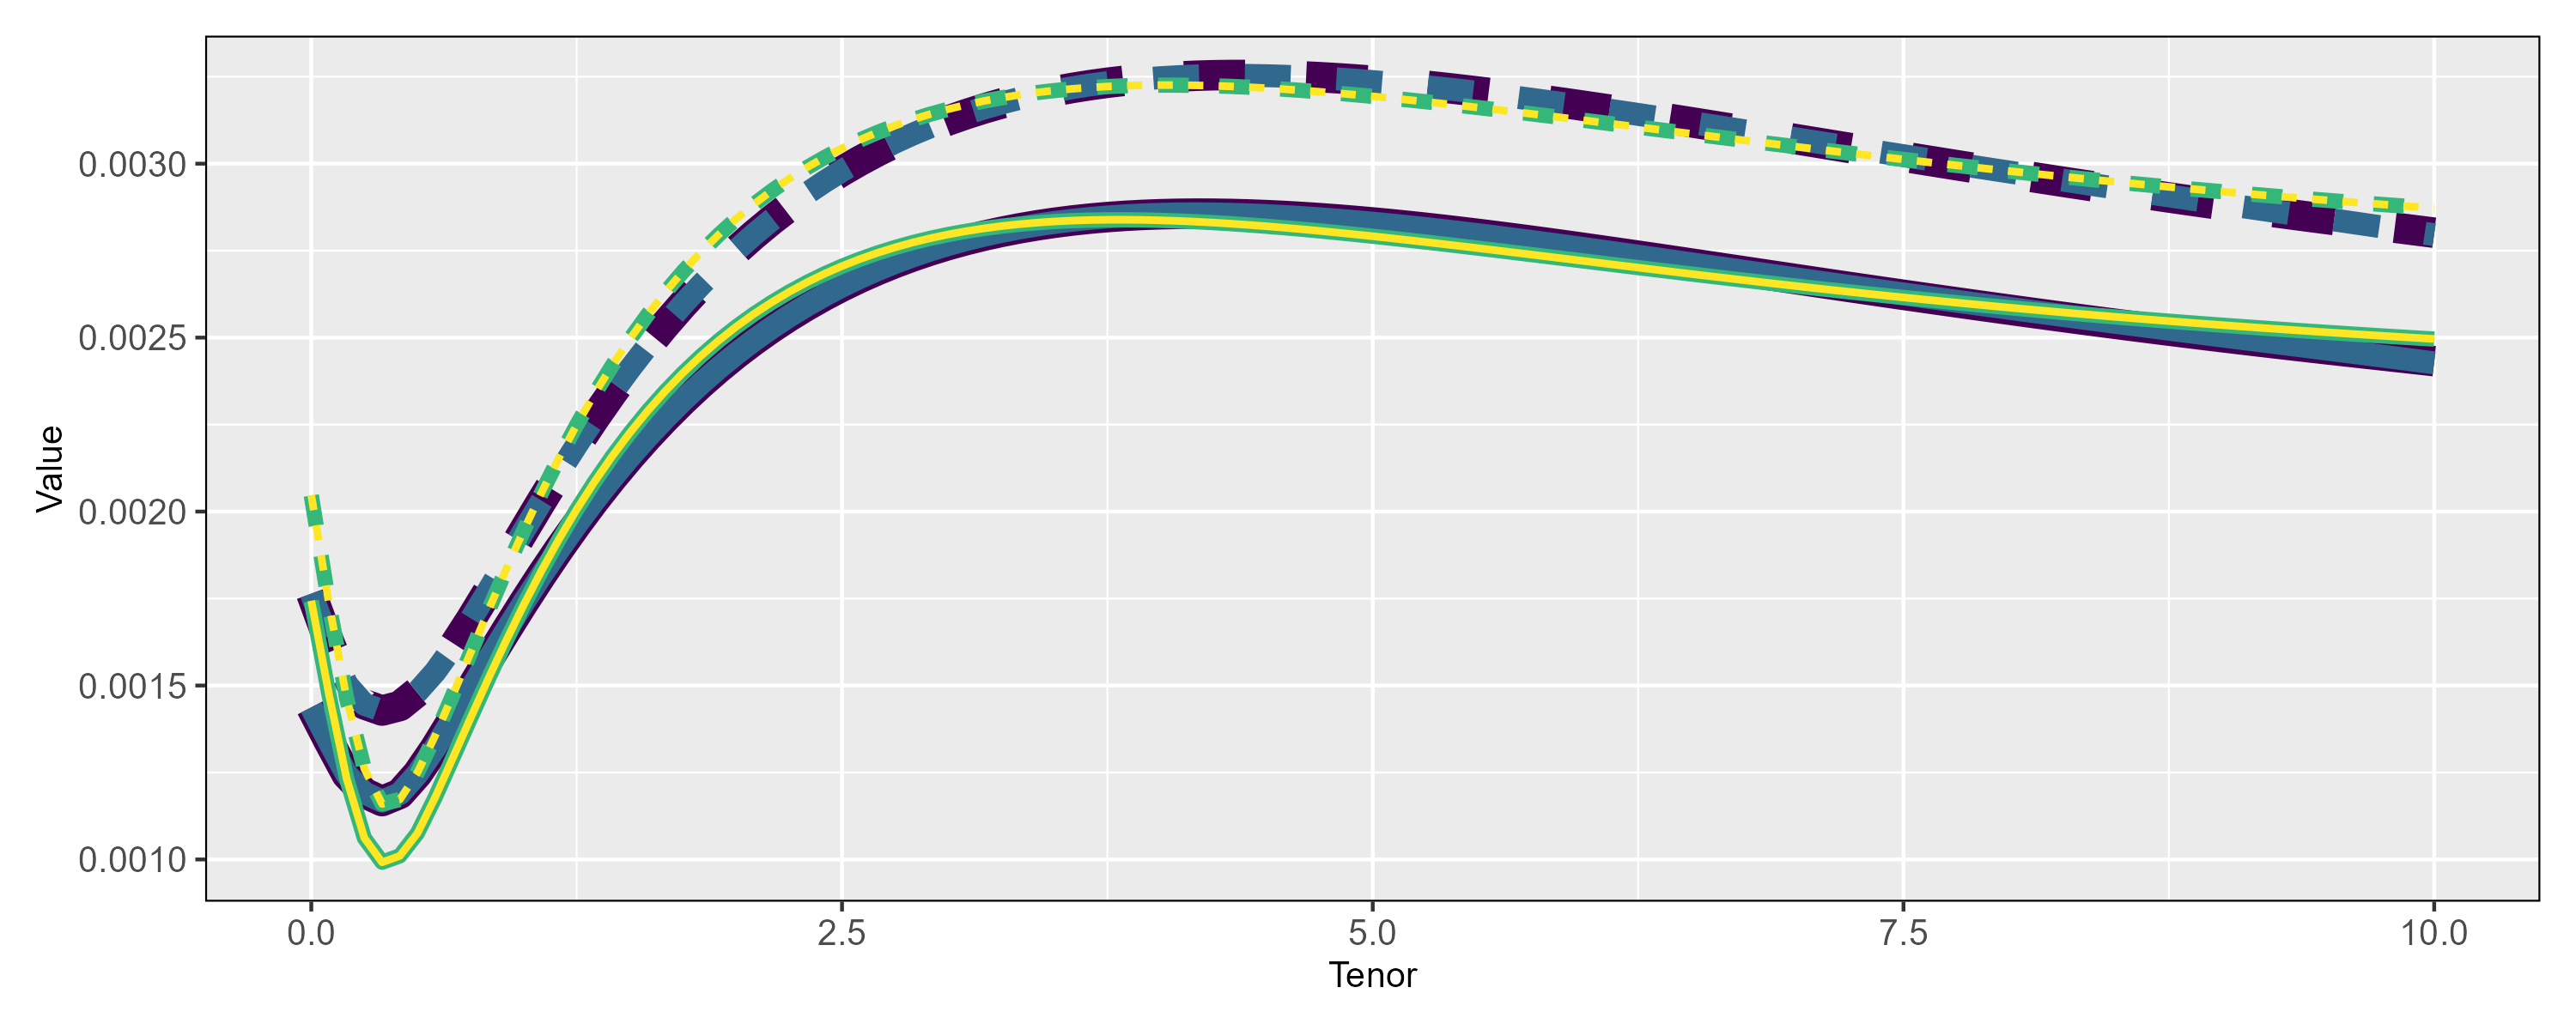
\includegraphics[width=.95\linewidth]{Figures/Error/zero_coupon_yields_phase_3_HJM_2F_LGOCV_small_error_plot.png}
    \caption[LGOCV errors for the four different models.]{LGOCV errors for the four different models. The solid lines are the MAPEs and the dashed lines are the MRSPEs. The \textbf{yellow} $\bigl($\textcolor{yellow_}{\textbf{---}}$\bigr)$ and \textbf{green} $\bigl($\textcolor{green_}{\textbf{---}}$\bigr)$ colored lines are obtained from procedure $1$ and fitted using a cubic polynomial and a natural cubic spline respectively. The \textbf{dark blue} $\bigl($\textcolor{dark_blue_1}{\textbf{---}}$\bigr)$ and \textbf{dark purple} $\bigl($\textcolor{dark_purple_}{\textbf{---}}$\bigr)$ colored lines are obtained from procedure $2$ and fitted using a cubic polynomial and a natural cubic spline respectively.}
    \label{fig:Error}
\end{figure}

\newpage

\section{Simulation}
 
\noindent The means of the realizations from the polynomial and spline models without extrapolation are shown in Figures \ref{fig:mean realizations of poly wo extrapolation, 10 years into the future.} and \ref{fig:mean realizations of spline wo extrapolation, 10 years into the future.} respectively. They show the same pattern, where the interest rates with short tenors decrease slowly until the other rates becomes larger. They then begin to rise slowly. At the end of the simulations, we can see that the $10$-year interest rate begin to flatten, and the simulations from the spline model starts to flatten earlier than the polynomial model.

\begin{figure}[!htbp]
    \centering
    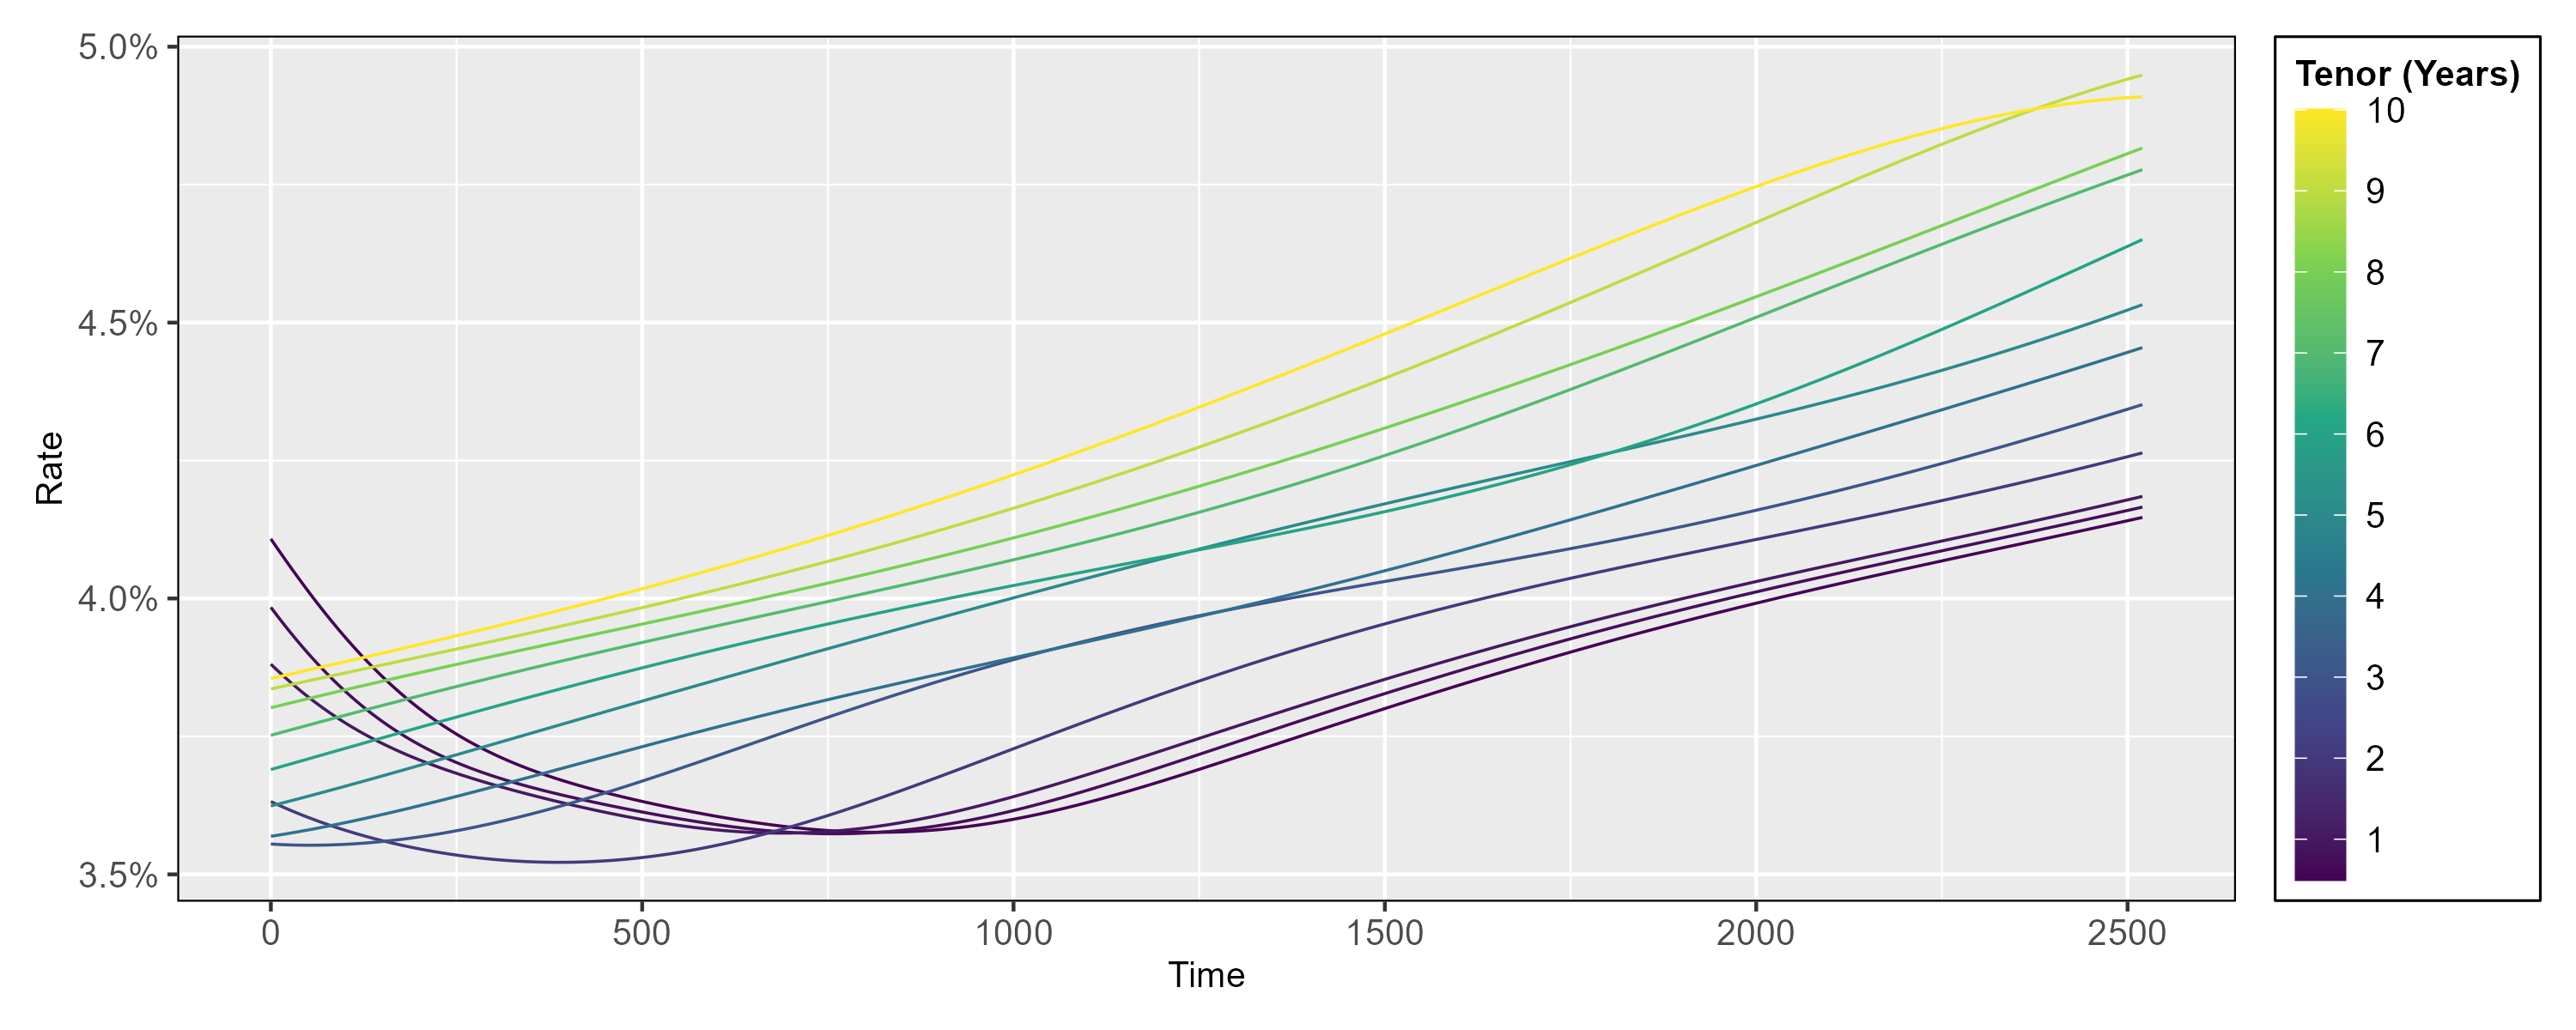
\includegraphics[width=.95\linewidth]{Figures/Simulated Interest Rates/zero_coupon_yields_phase_3_HJM_2F_poly_model_simulated_10Y_mean_small_time_plot.png}
    
    \caption[Mean of the realizations, Polynomial Model]{Means of the realizations from the polynomial model.}
    \label{fig:mean realizations of poly wo extrapolation, 10 years into the future.}
\end{figure}

\begin{figure}[!htbp]
    \centering
    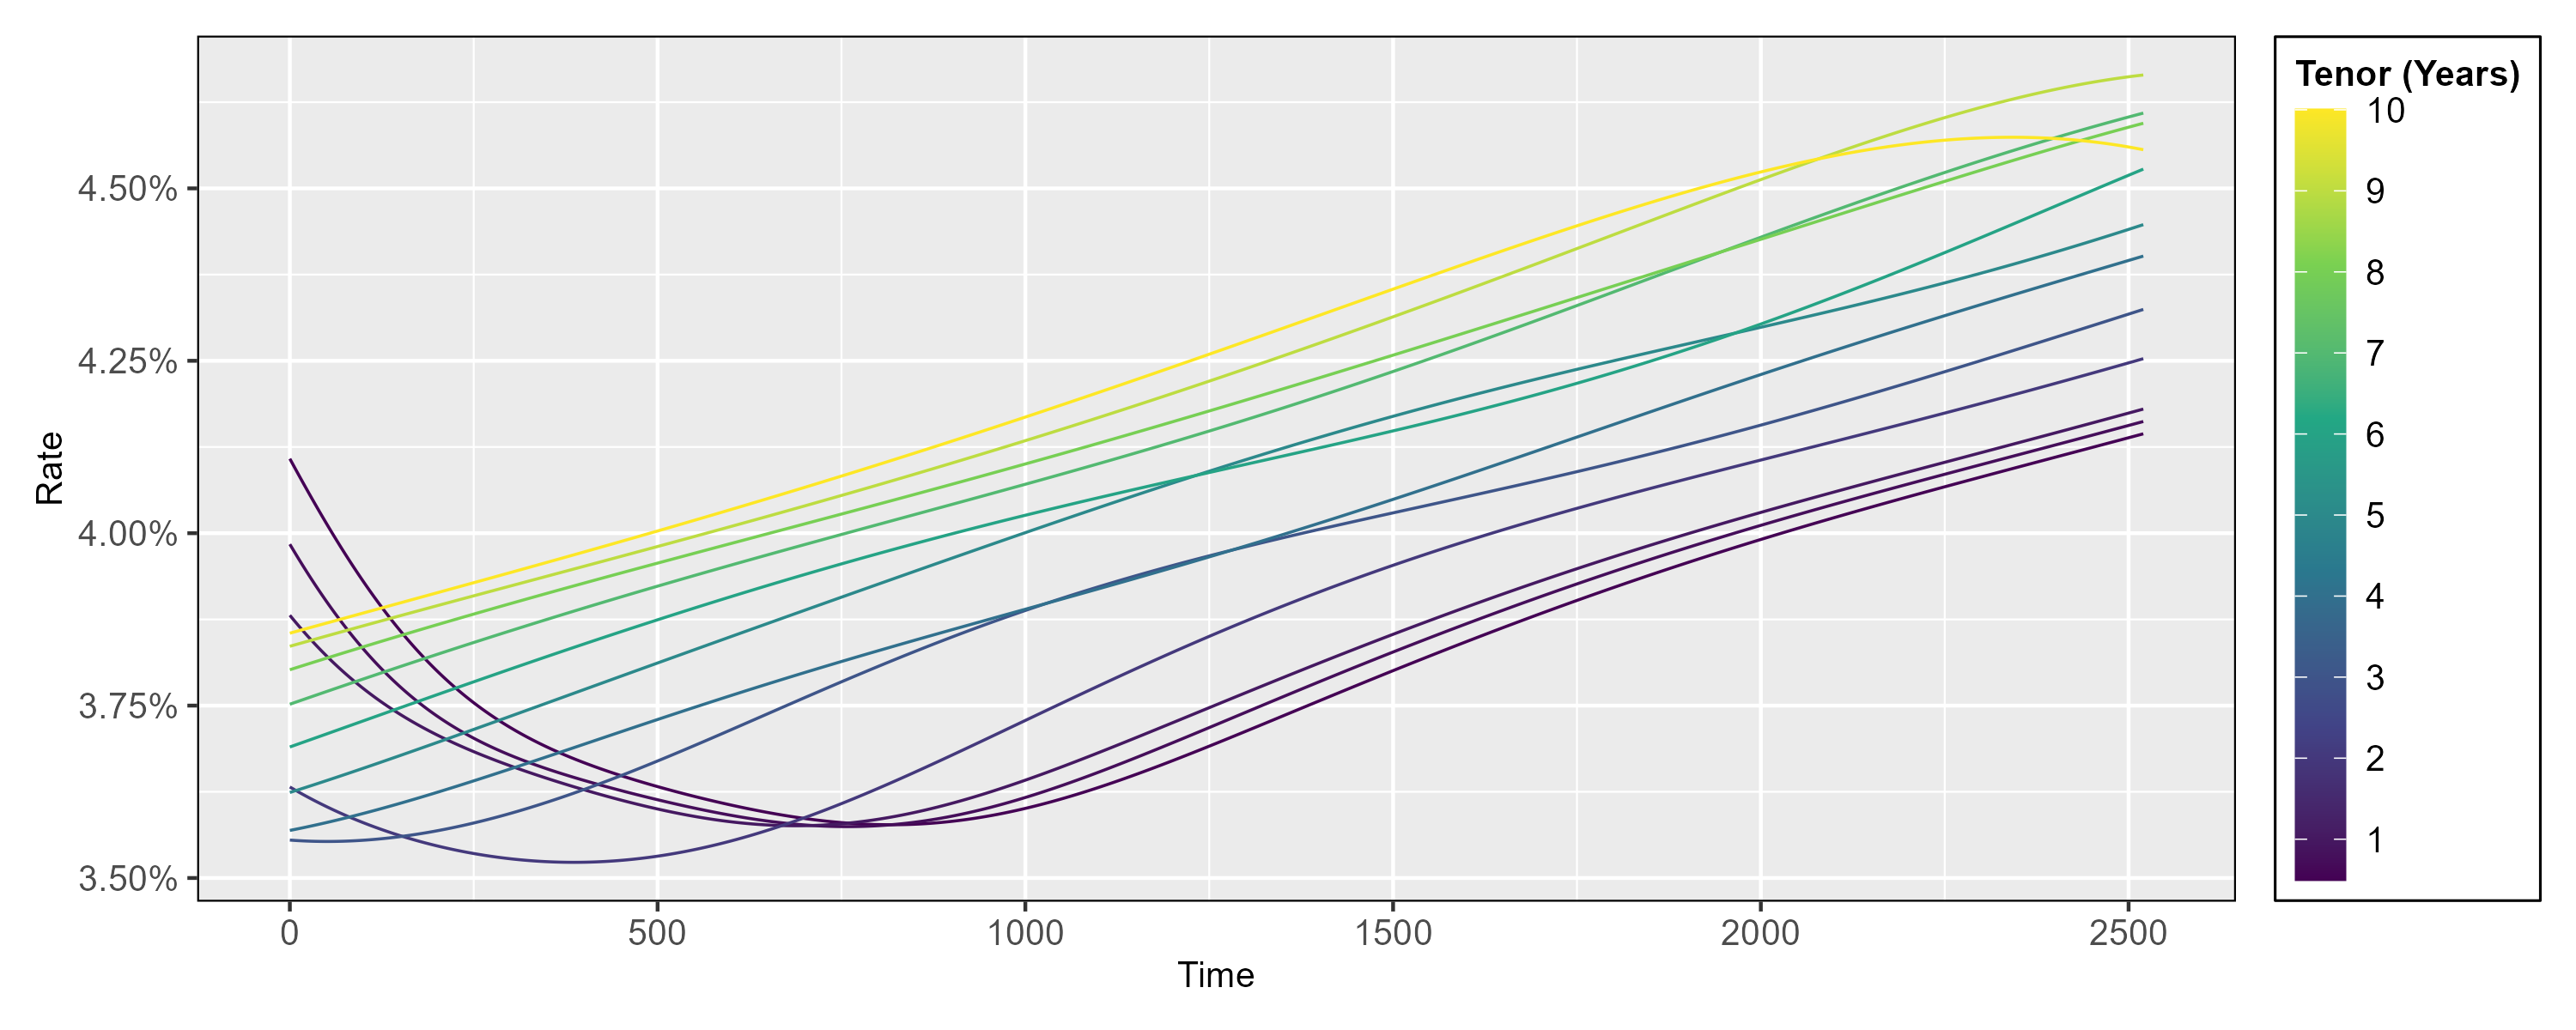
\includegraphics[width=.95\linewidth]{Figures/Simulated Interest Rates/zero_coupon_yields_phase_3_HJM_2F_spline_model_simulated_10Y_mean_small_time_plot.png}
    
    \caption[Mean of the realizations, Spline Model]{Means of the realizations from the spline model.}
    \label{fig:mean realizations of spline wo extrapolation, 10 years into the future.}
\end{figure}

\newpage

The means of the realizations from the polynomial and spline models using procedure $1$ are shown in Figures \ref{fig:mean realizations of procedure 1, poly, 10 years into the future.} and \ref{fig:mean realizations of procedure 1, spline, 10 years into the future.} respectively. They both show many distinct discontinuities at short tenors.

\begin{figure}[!htbp]
    \centering
    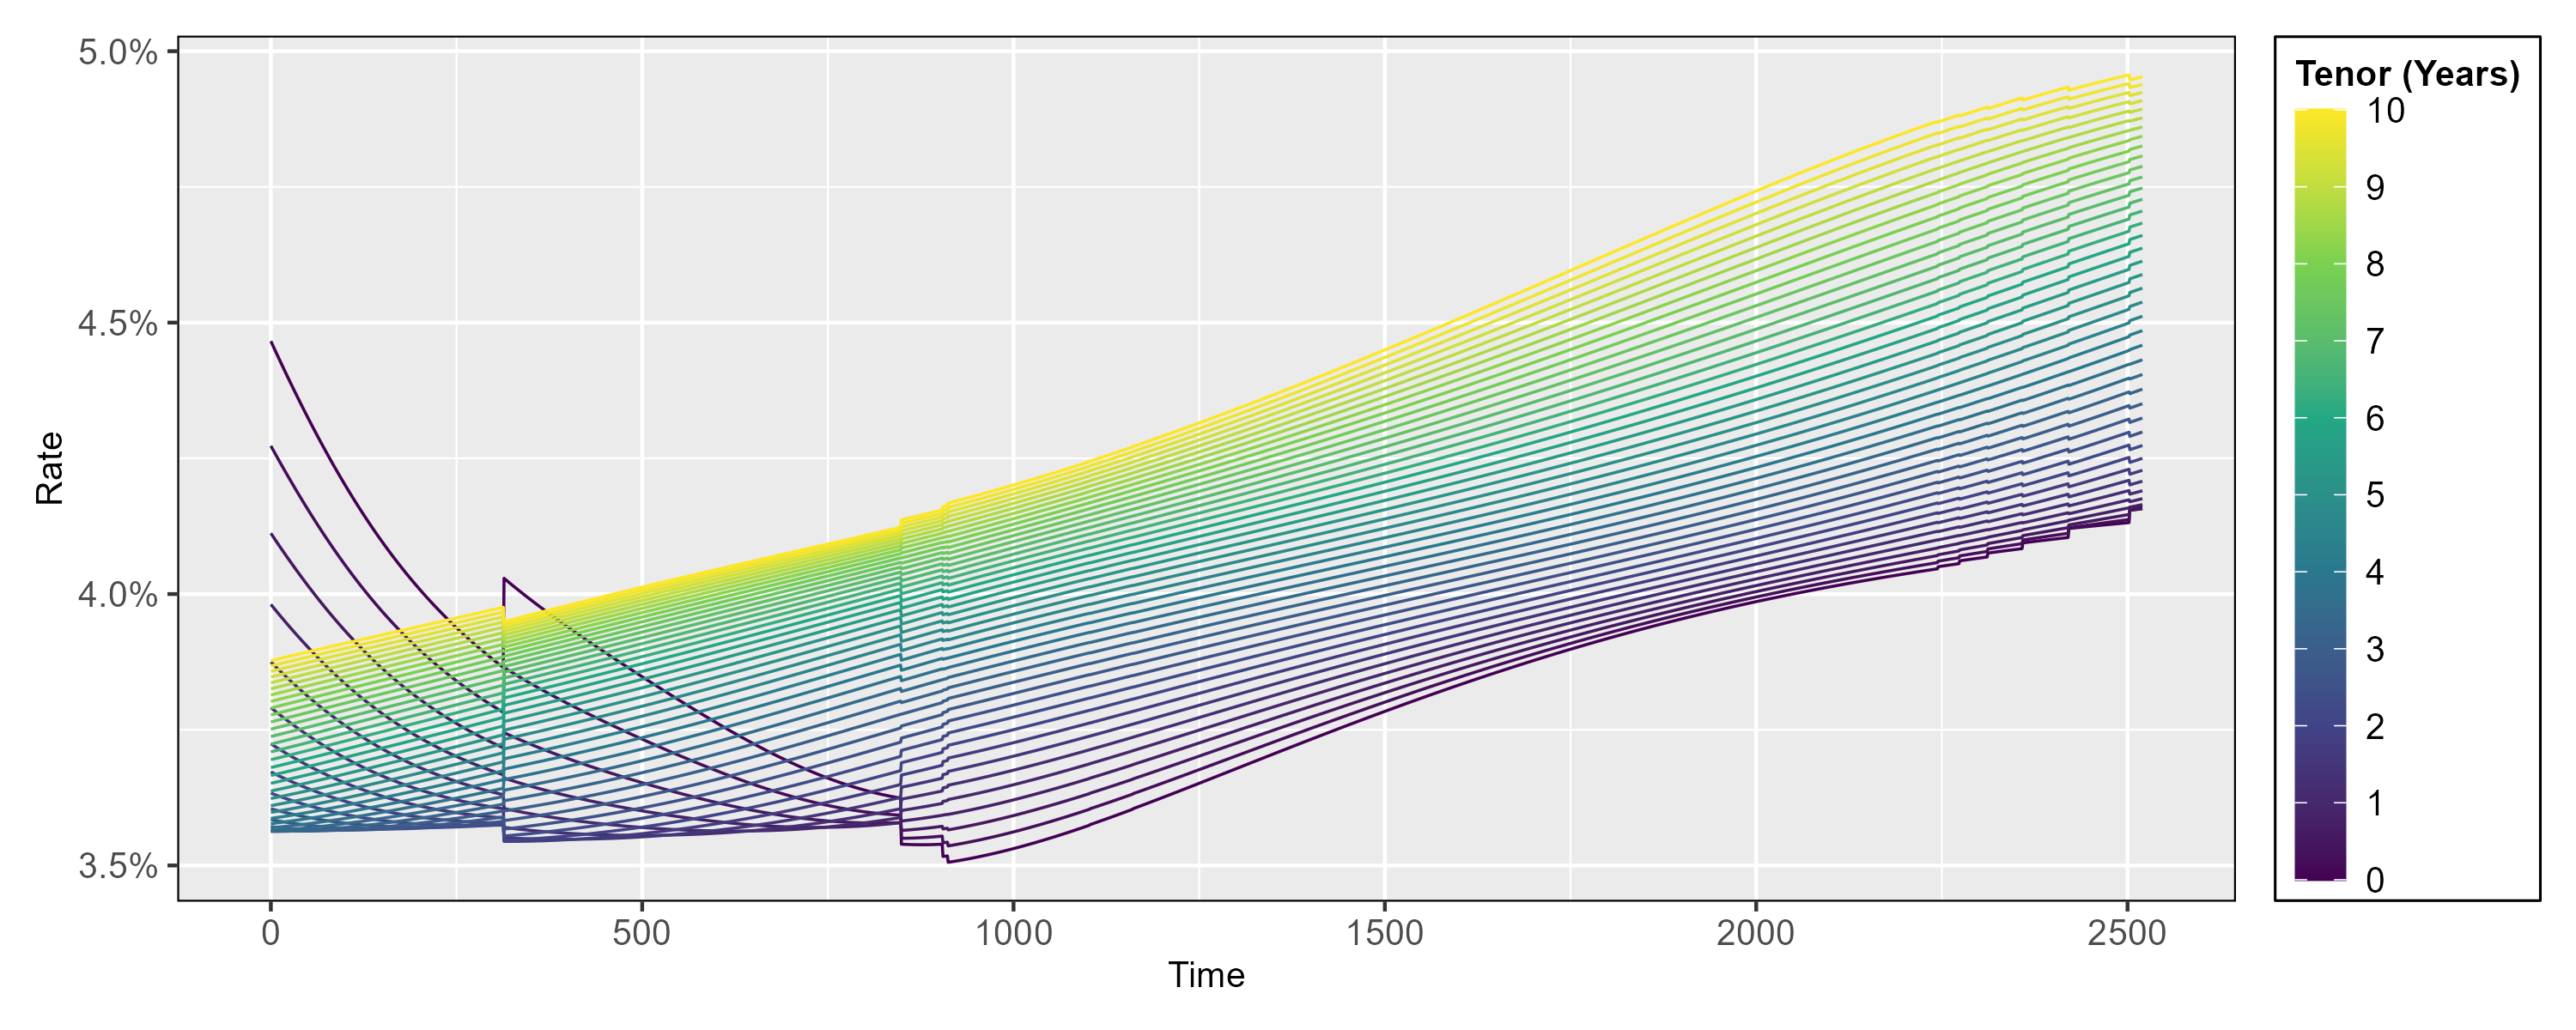
\includegraphics[width=.95\linewidth]{Figures/Simulated Interest Rates/zero_coupon_yields_phase_3_HJM_2F_procedure_1_poly_model_simulated_10Y_mean_small_time_plot.png}
    
    \caption[Mean of the realizations, Polynomial Model, Procedure 1]{Means of the realizations from the polynomial model using procedure 1. Generated in $4036$ seconds.}
    \label{fig:mean realizations of procedure 1, poly, 10 years into the future.}
\end{figure}

\begin{figure}[!htbp]
    \centering
    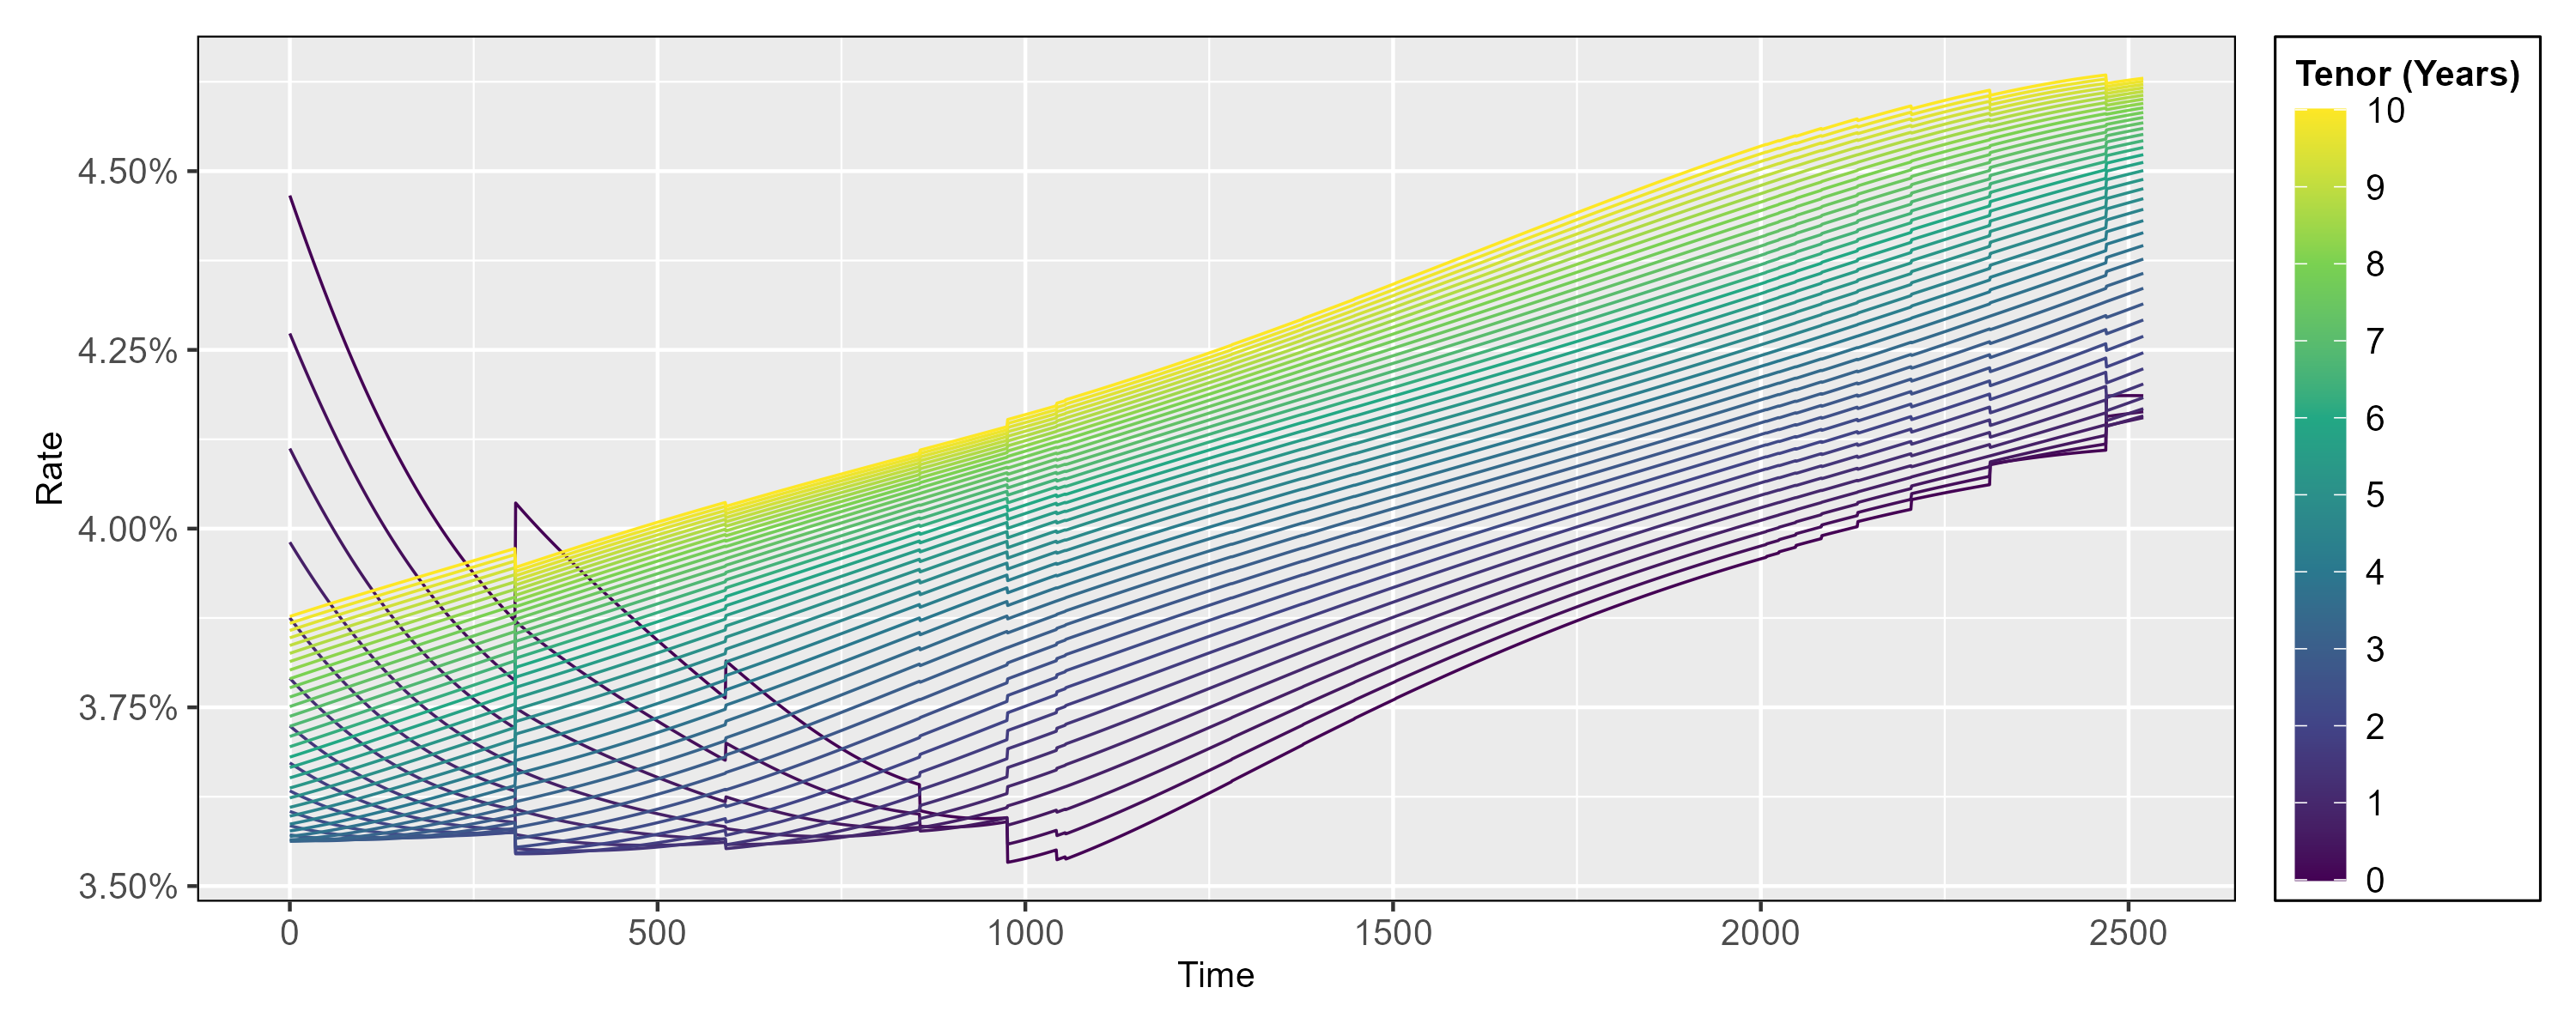
\includegraphics[width=.95\linewidth]{Figures/Simulated Interest Rates/zero_coupon_yields_phase_3_HJM_2F_procedure_1_spline_model_simulated_10Y_mean_small_time_plot.png}
    
    \caption[Mean of the realizations, Spline Model, Procedure 1]{Means of the realizations from the spline model using procedure 1. Generated in $4145$ seconds.}
    \label{fig:mean realizations of procedure 1, spline, 10 years into the future.}
\end{figure}

\newpage

The means of the realizations from the polynomial and spline models using procedure $2$ are shown in Figures \ref{fig:mean realizations of procedure 2, poly, 10 years into the future.} and \ref{fig:mean realizations of procedure 2, spline, 10 years into the future.} respectively. They both show the exact same pattern for all the tenors, but the polynomial model has a slightly higher expected value in $10$ years.

\begin{figure}[!htbp]
    \centering
    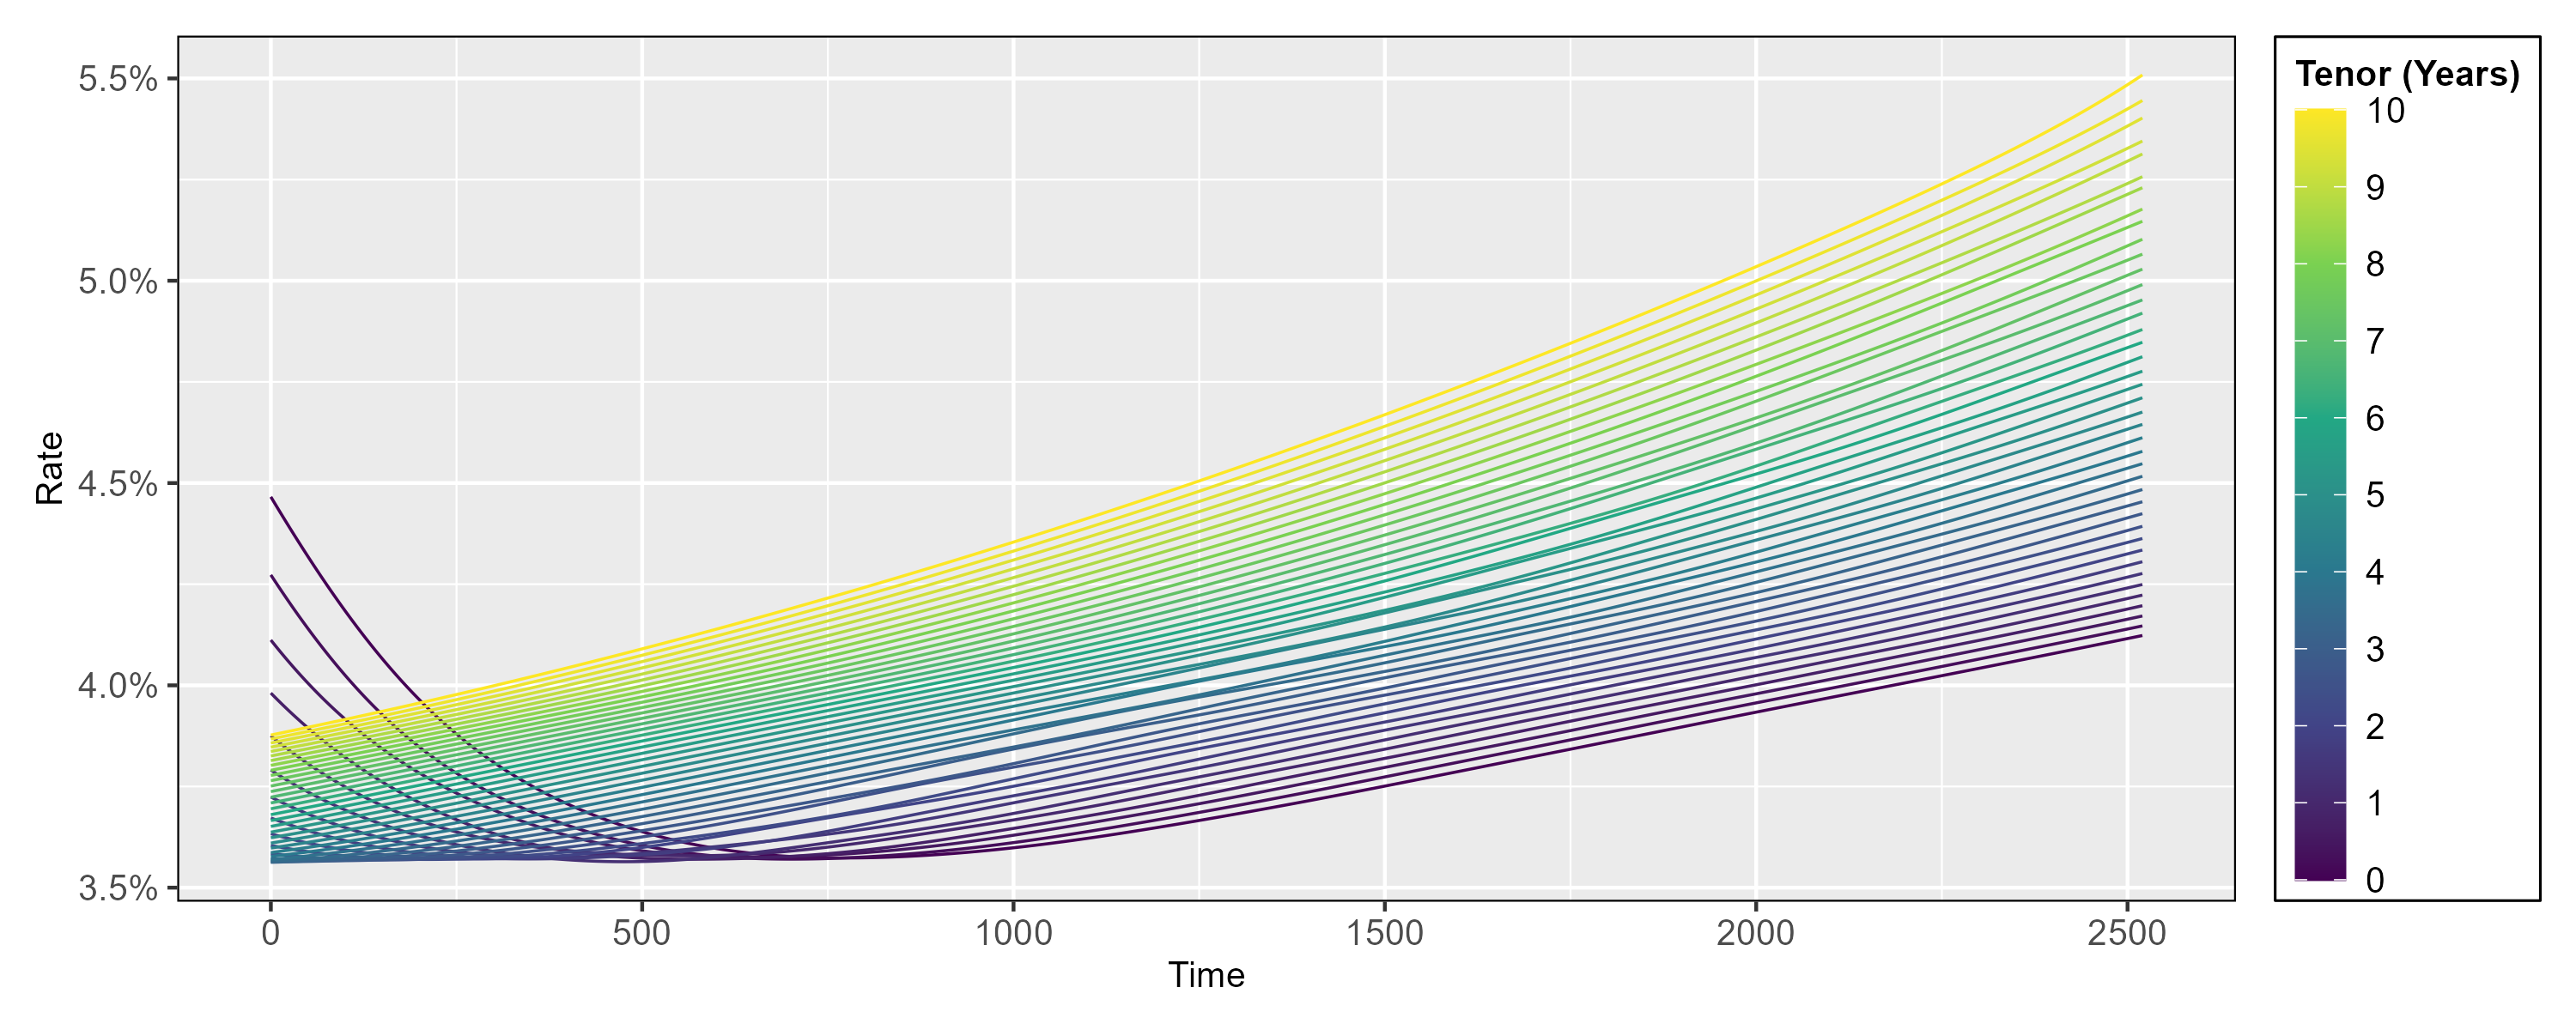
\includegraphics[width=.95\linewidth]{Figures/Simulated Interest Rates/zero_coupon_yields_phase_3_HJM_2F_procedure_2_poly_model_simulated_10Y_mean_small_time_plot.png}
    
    \caption[Mean of the realizations, Polynomial Model, Procedure 2]{Means of the realizations from the polynomial model using procedure 2. Generated in $264$ seconds.}
    \label{fig:mean realizations of procedure 2, poly, 10 years into the future.}
\end{figure}

\begin{figure}[!htbp]
    \centering
    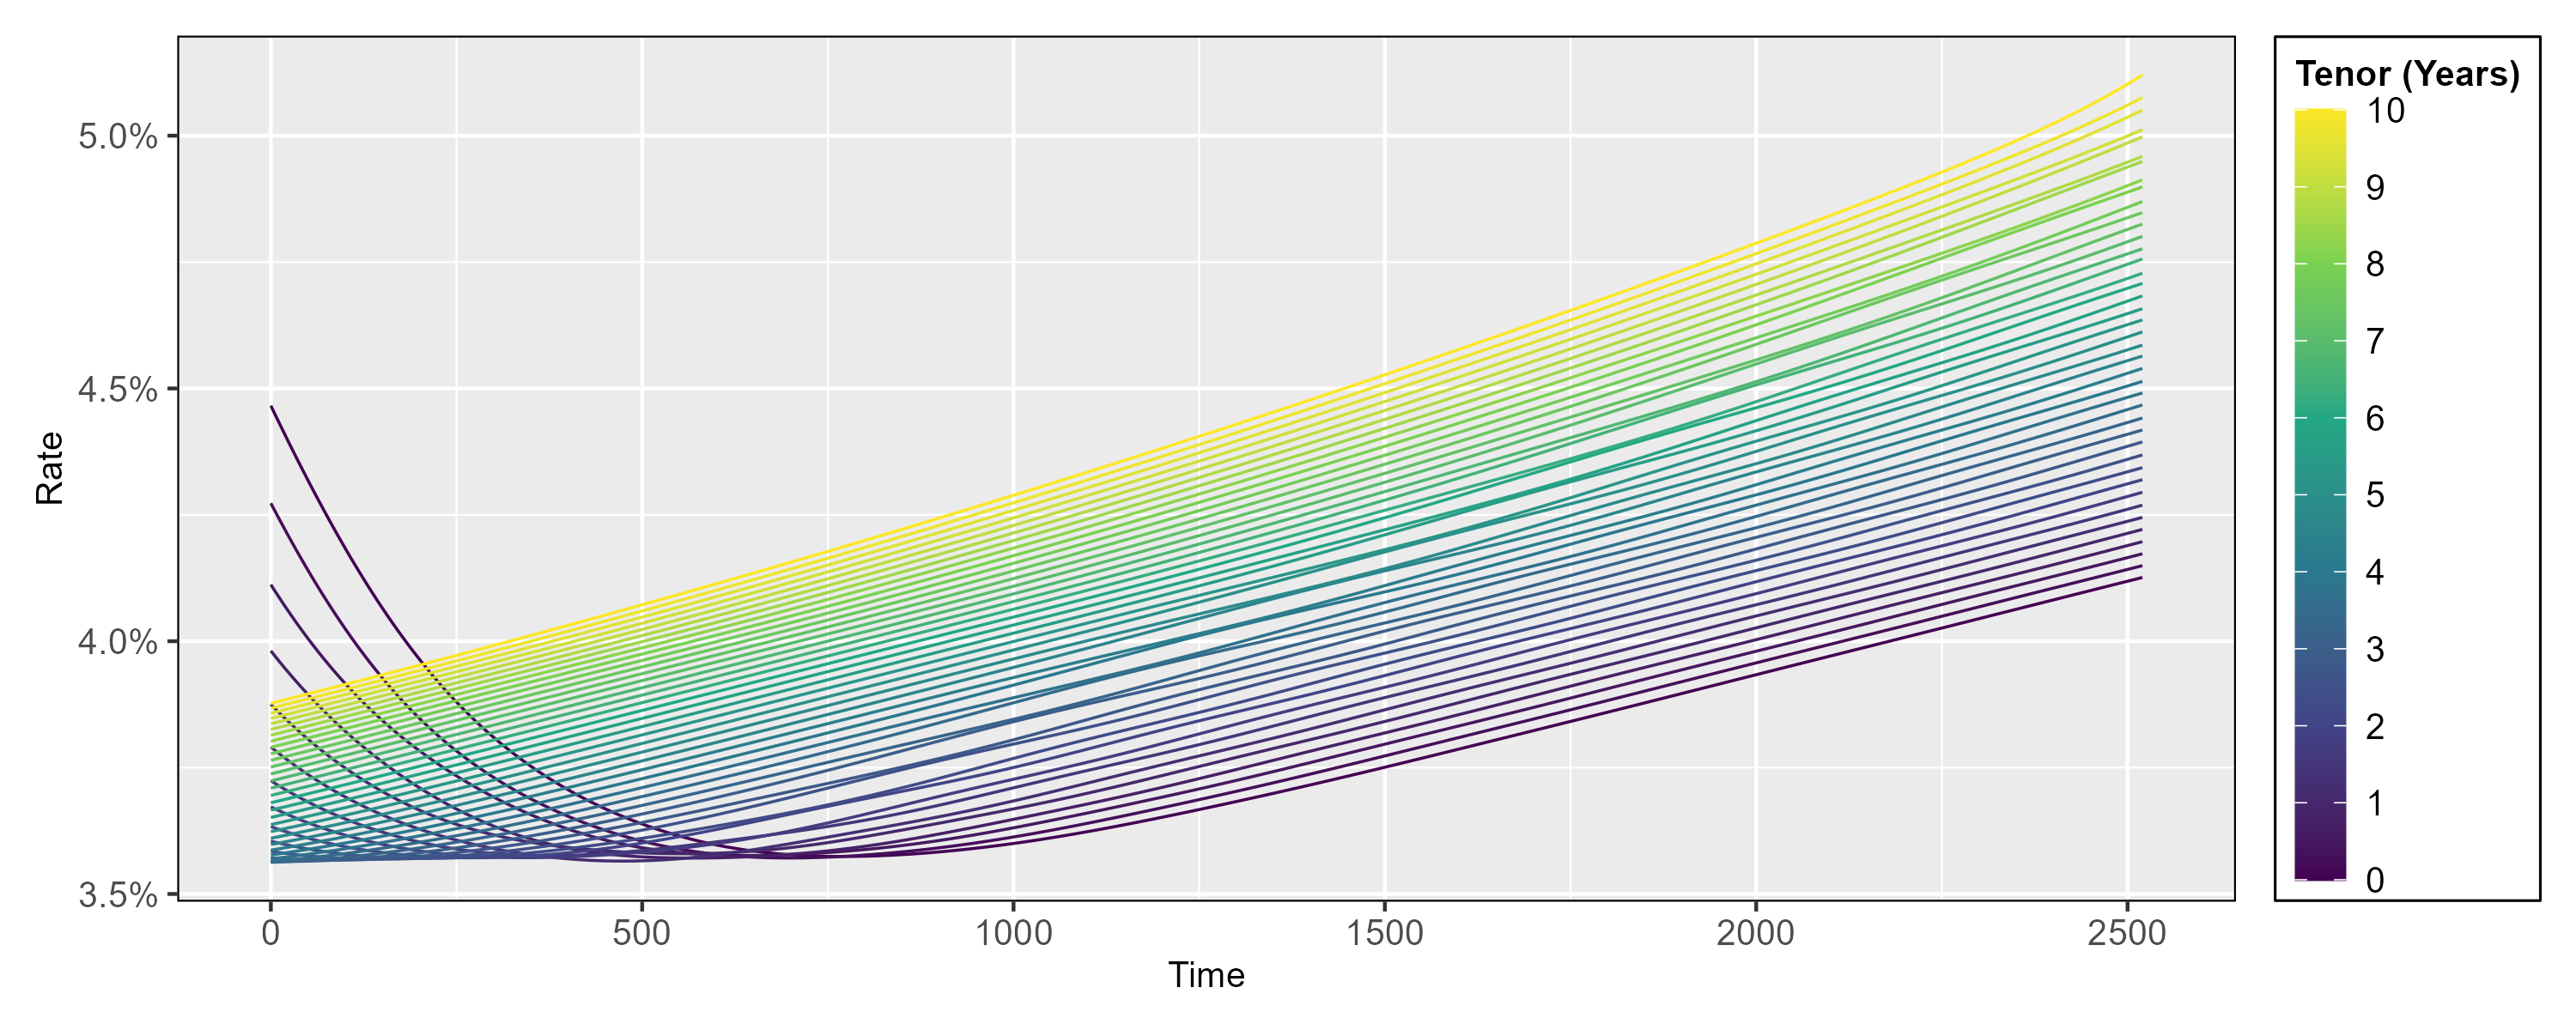
\includegraphics[width=.95\linewidth]{Figures/Simulated Interest Rates/zero_coupon_yields_phase_3_HJM_2F_procedure_2_spline_model_simulated_10Y_mean_small_time_plot.png}
    
    \caption[Mean of the realizations, Spline Model, Procedure 2]{Means of the realizations from the spline model using procedure 2. Generated in $265$ seconds.}
    \label{fig:mean realizations of procedure 2, spline, 10 years into the future.}
\end{figure}


\newpage






\newpage

\section{Derivative Price and Risk}

\noindent Using the realizations generated using procedures $1$ and $2$ I have calculated the price of fixed-for-floating interest rates swaps, which are shown in Figure \ref{fig:irs prices}. The subplots show how the prices changes over time. They all look identical to each other, and they are converging to a price of $10$ at the end of the contract. The expected value does not reach zero at the start of the contract. The histograms of the prices as of April $30$, $2025$, are shown in Figure \ref{fig:irs prices hist today}. The prices generated from the polynomial model using procedure $1$ deviates slightly from the other three. It has a much wider confidence interval.

The expected exposure and the potential future exposure of the contracts are shown in Figure \ref{fig:exposure}. Again we see that they give similar results.



\begin{figure}[!htbp]
    \centering
    \captionsetup{type=figure}
    \begin{subfigure}{0.49\textwidth}
        \centering
        \captionsetup{justification=centering}
        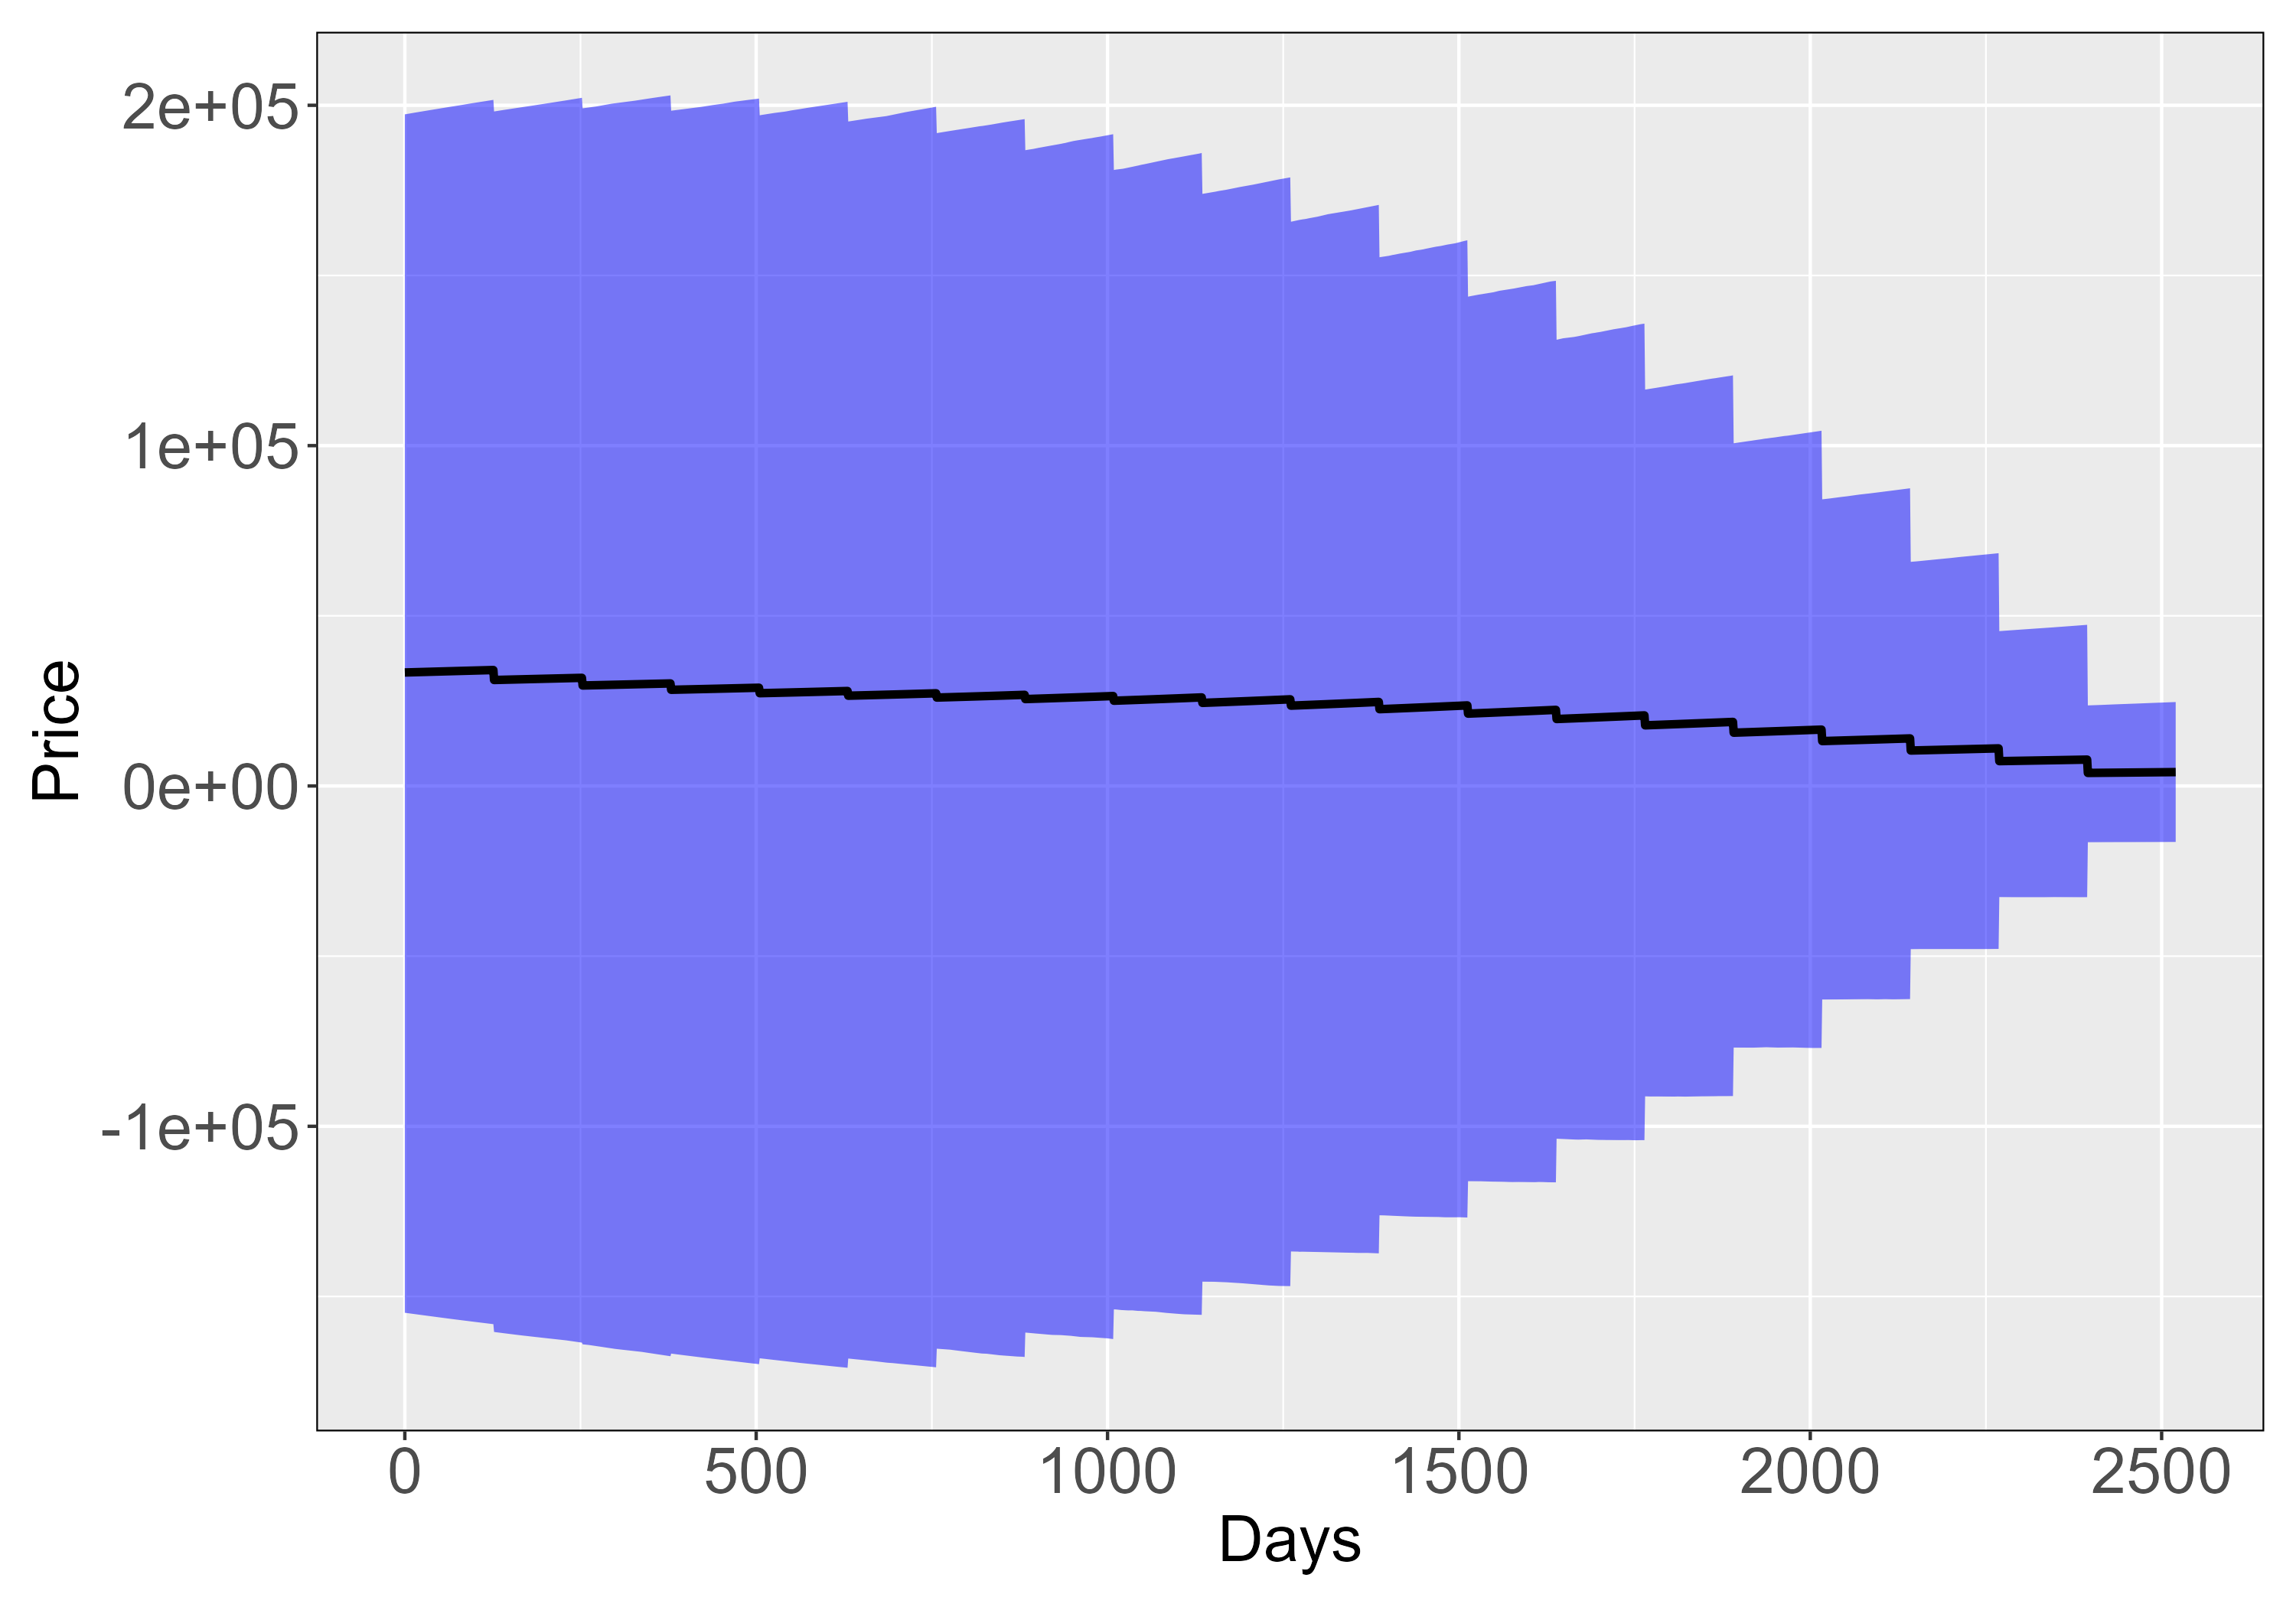
\includegraphics[width=\textwidth]{Figures/Prices/procedure_1_poly_model_prices_plot.png}
        \subcaption{Polynomial model using procedure 1.}
        \label{fig:irs of procedure 1, poly.}
    \end{subfigure}
    \hfill
    \begin{subfigure}{0.49\textwidth}
        \centering
        \captionsetup{justification=centering}
        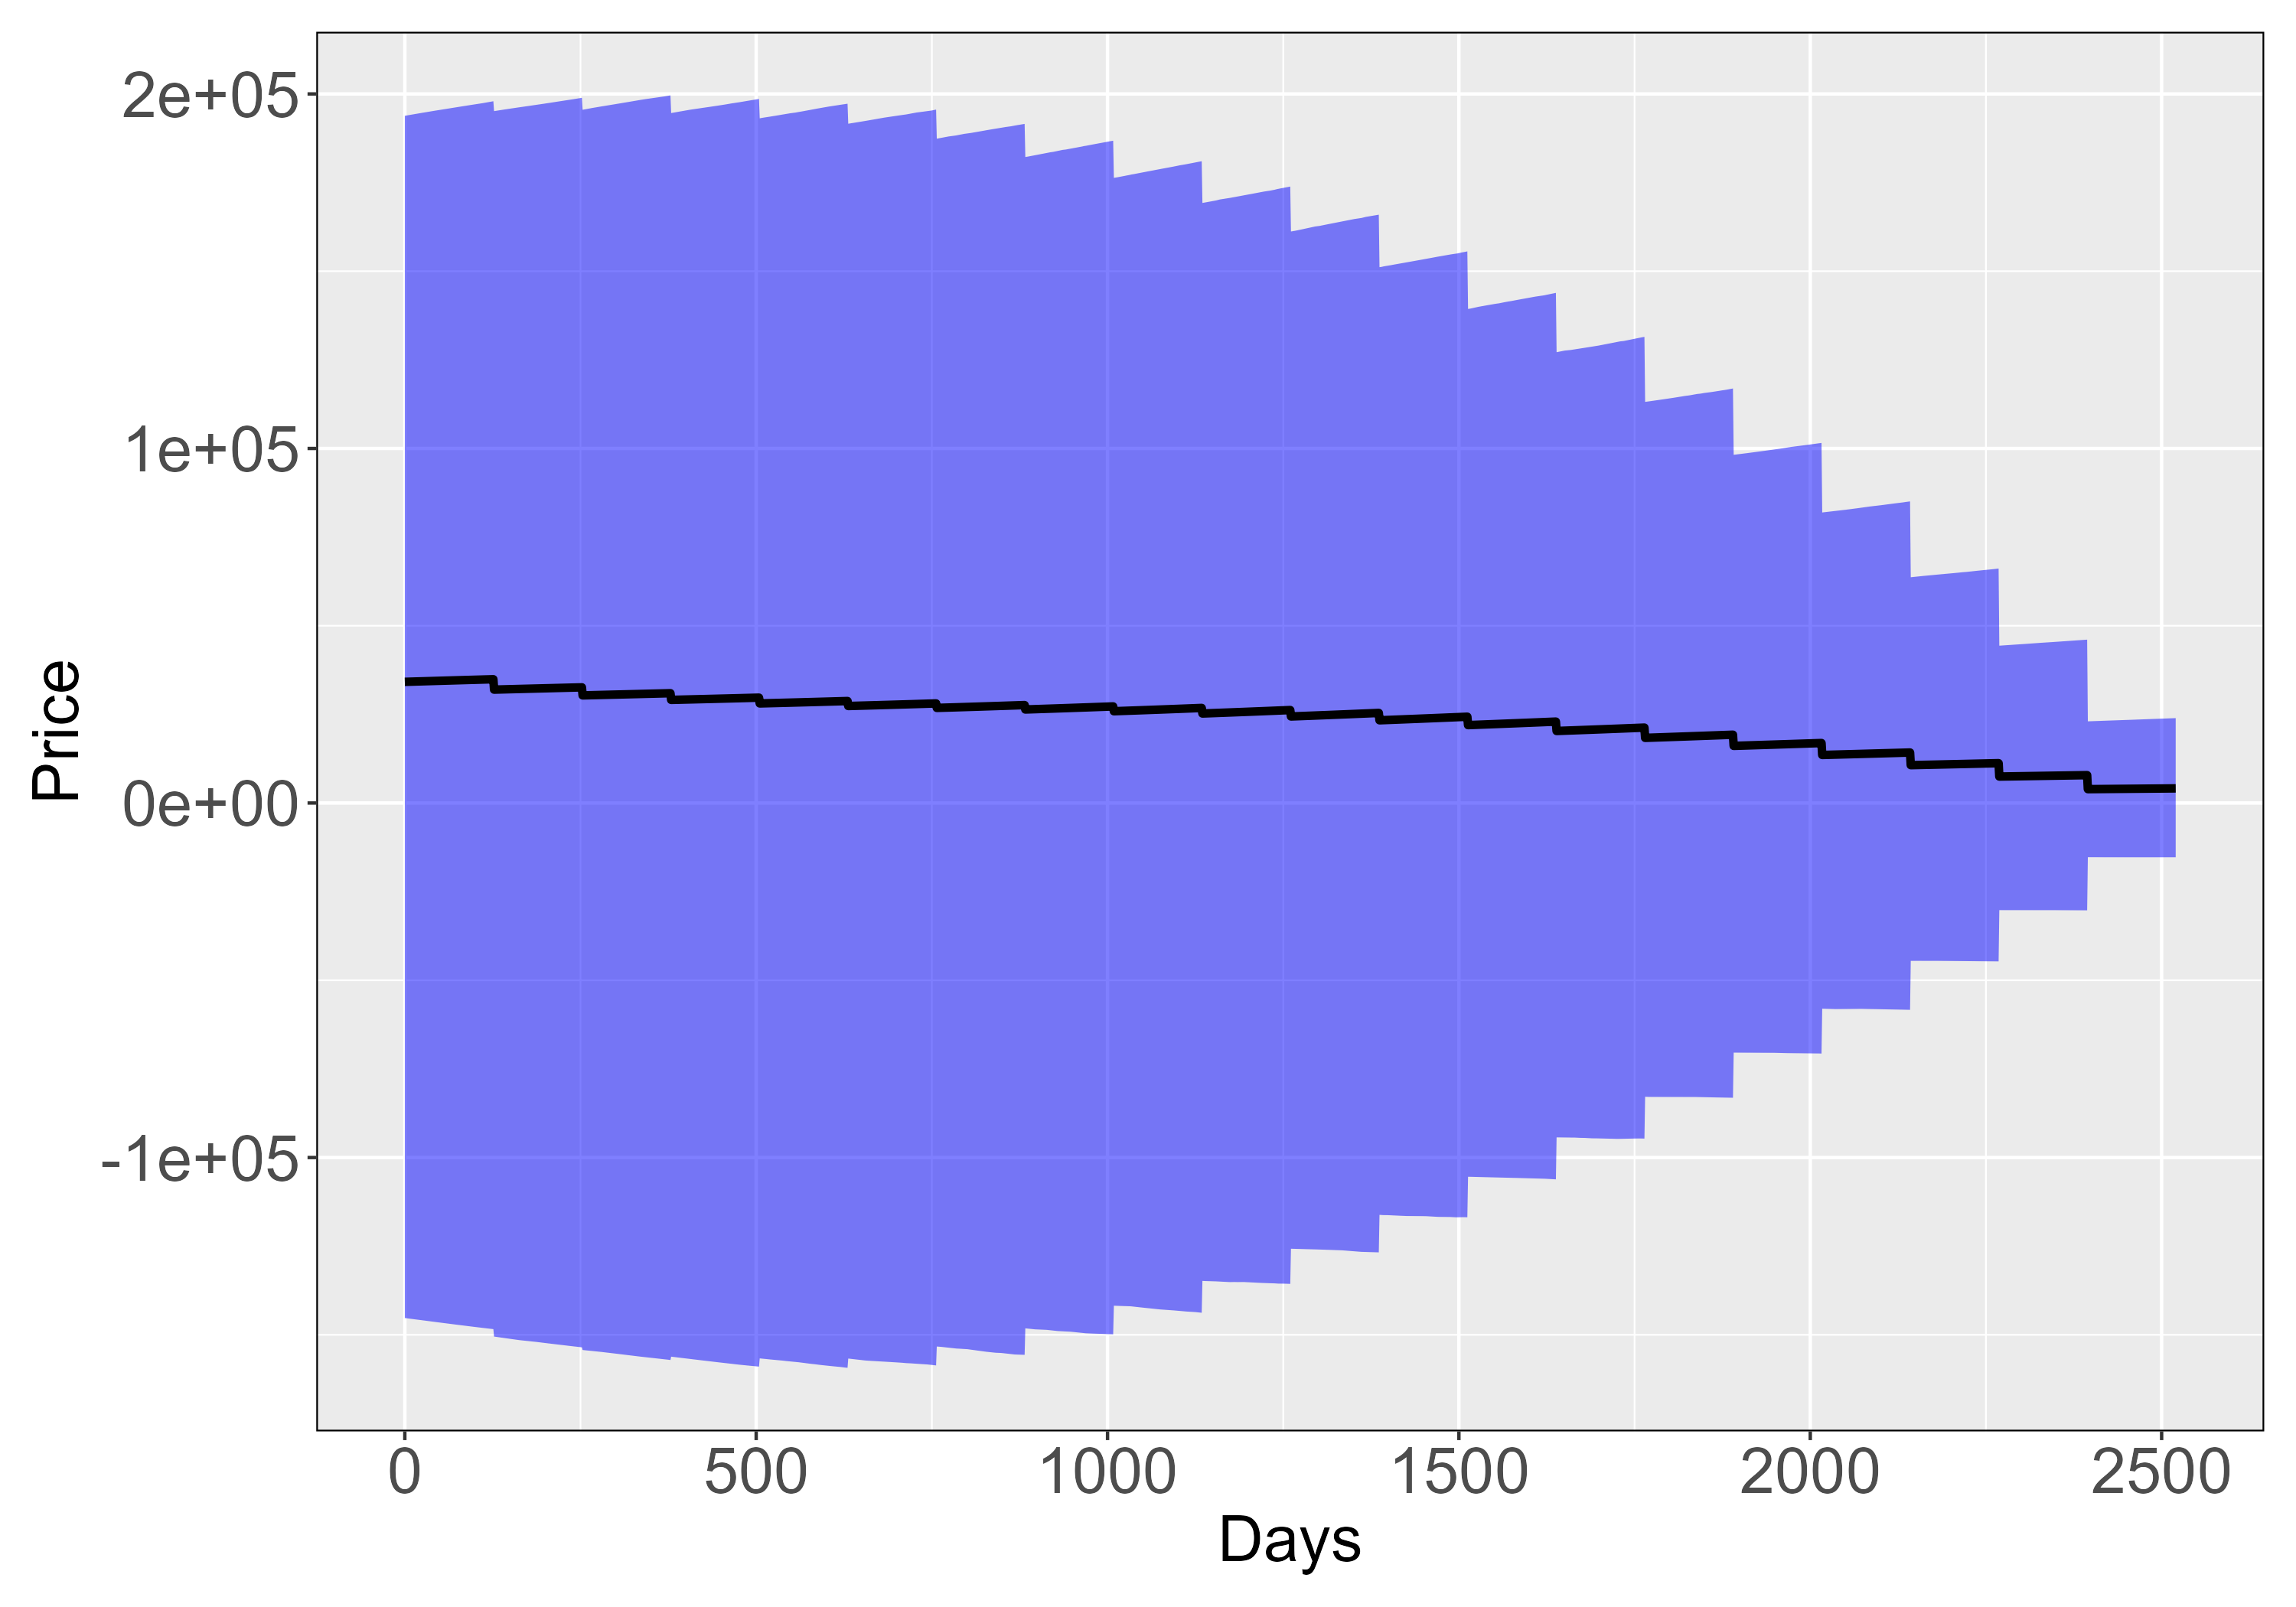
\includegraphics[width=\textwidth]{Figures/Prices/procedure_1_spline_model_prices_plot.png}
        \subcaption{Spline model using procedure 1.}
        \label{fig:irs of procedure 1, spline.}
    \end{subfigure}
    \vskip\baselineskip
    \begin{subfigure}{0.49\textwidth}
        \centering
        \captionsetup{justification=centering}
        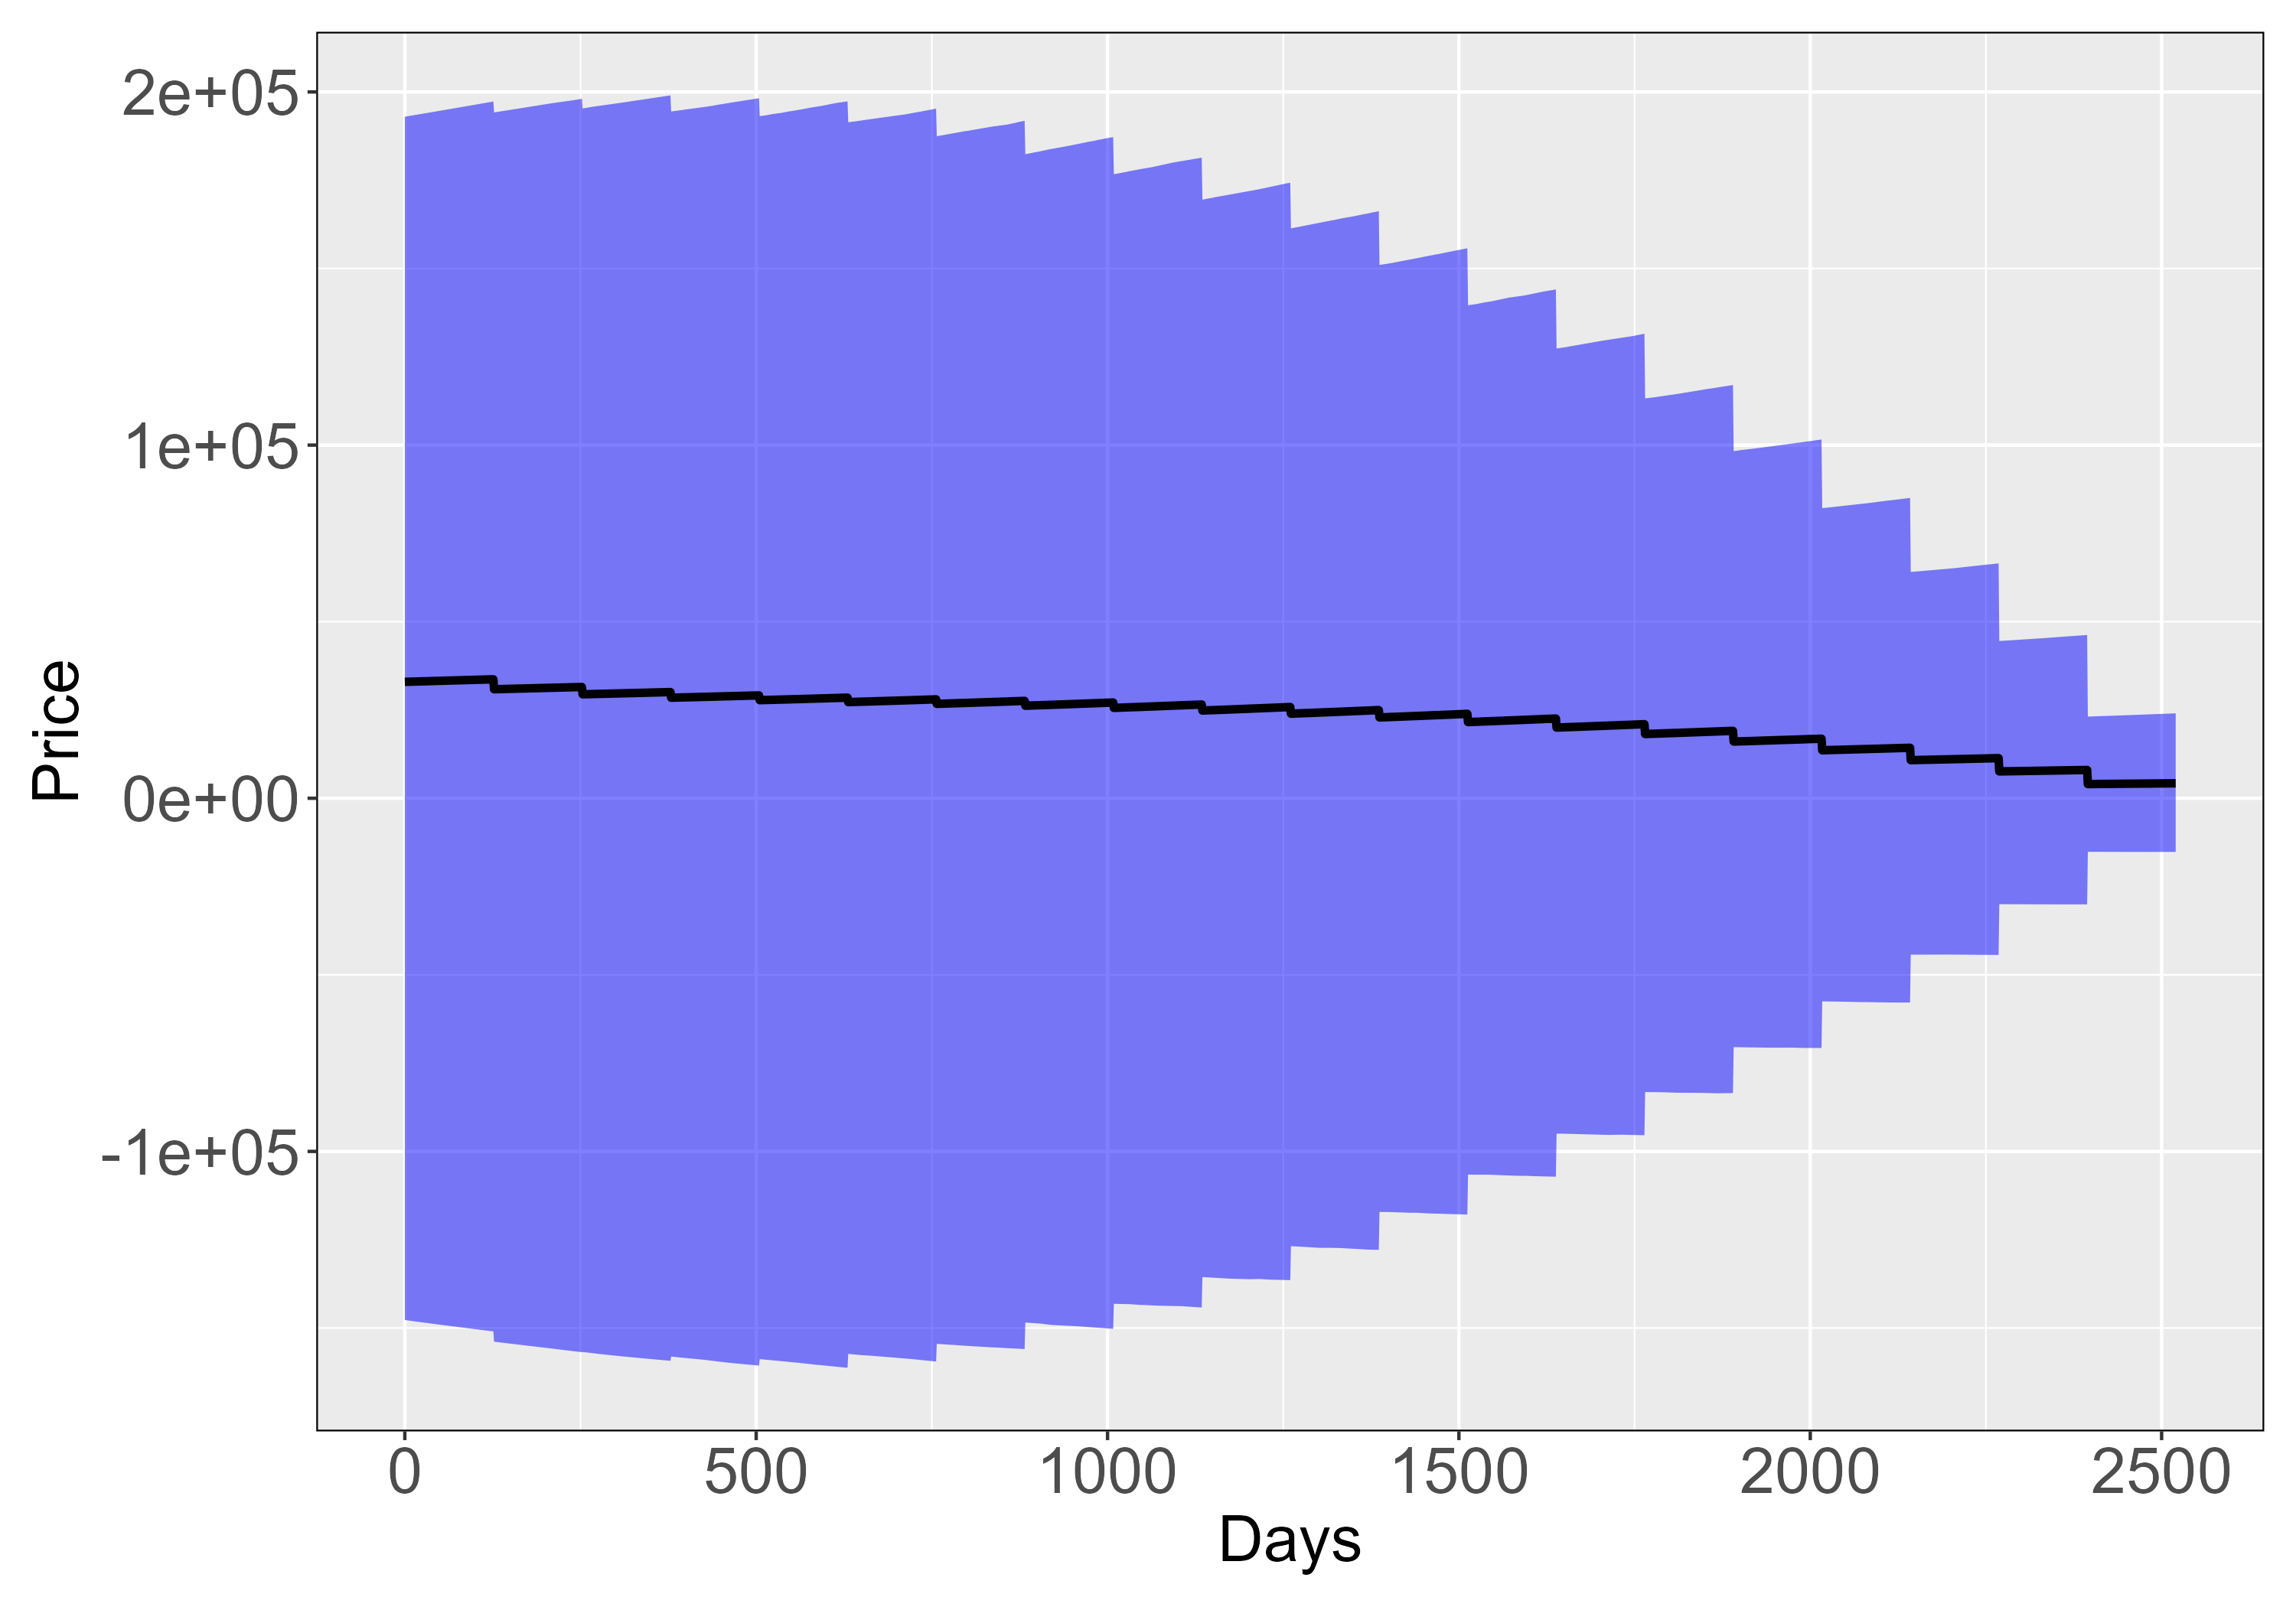
\includegraphics[width=\textwidth]{Figures/Prices/procedure_2_poly_model_prices_plot.png}
        \subcaption{Polynomial model using procedure 2.}
        \label{fig:irs of procedure 2, poly.}
    \end{subfigure}
    \hfill
    \begin{subfigure}{0.49\textwidth}
        \centering
        \captionsetup{justification=centering}
        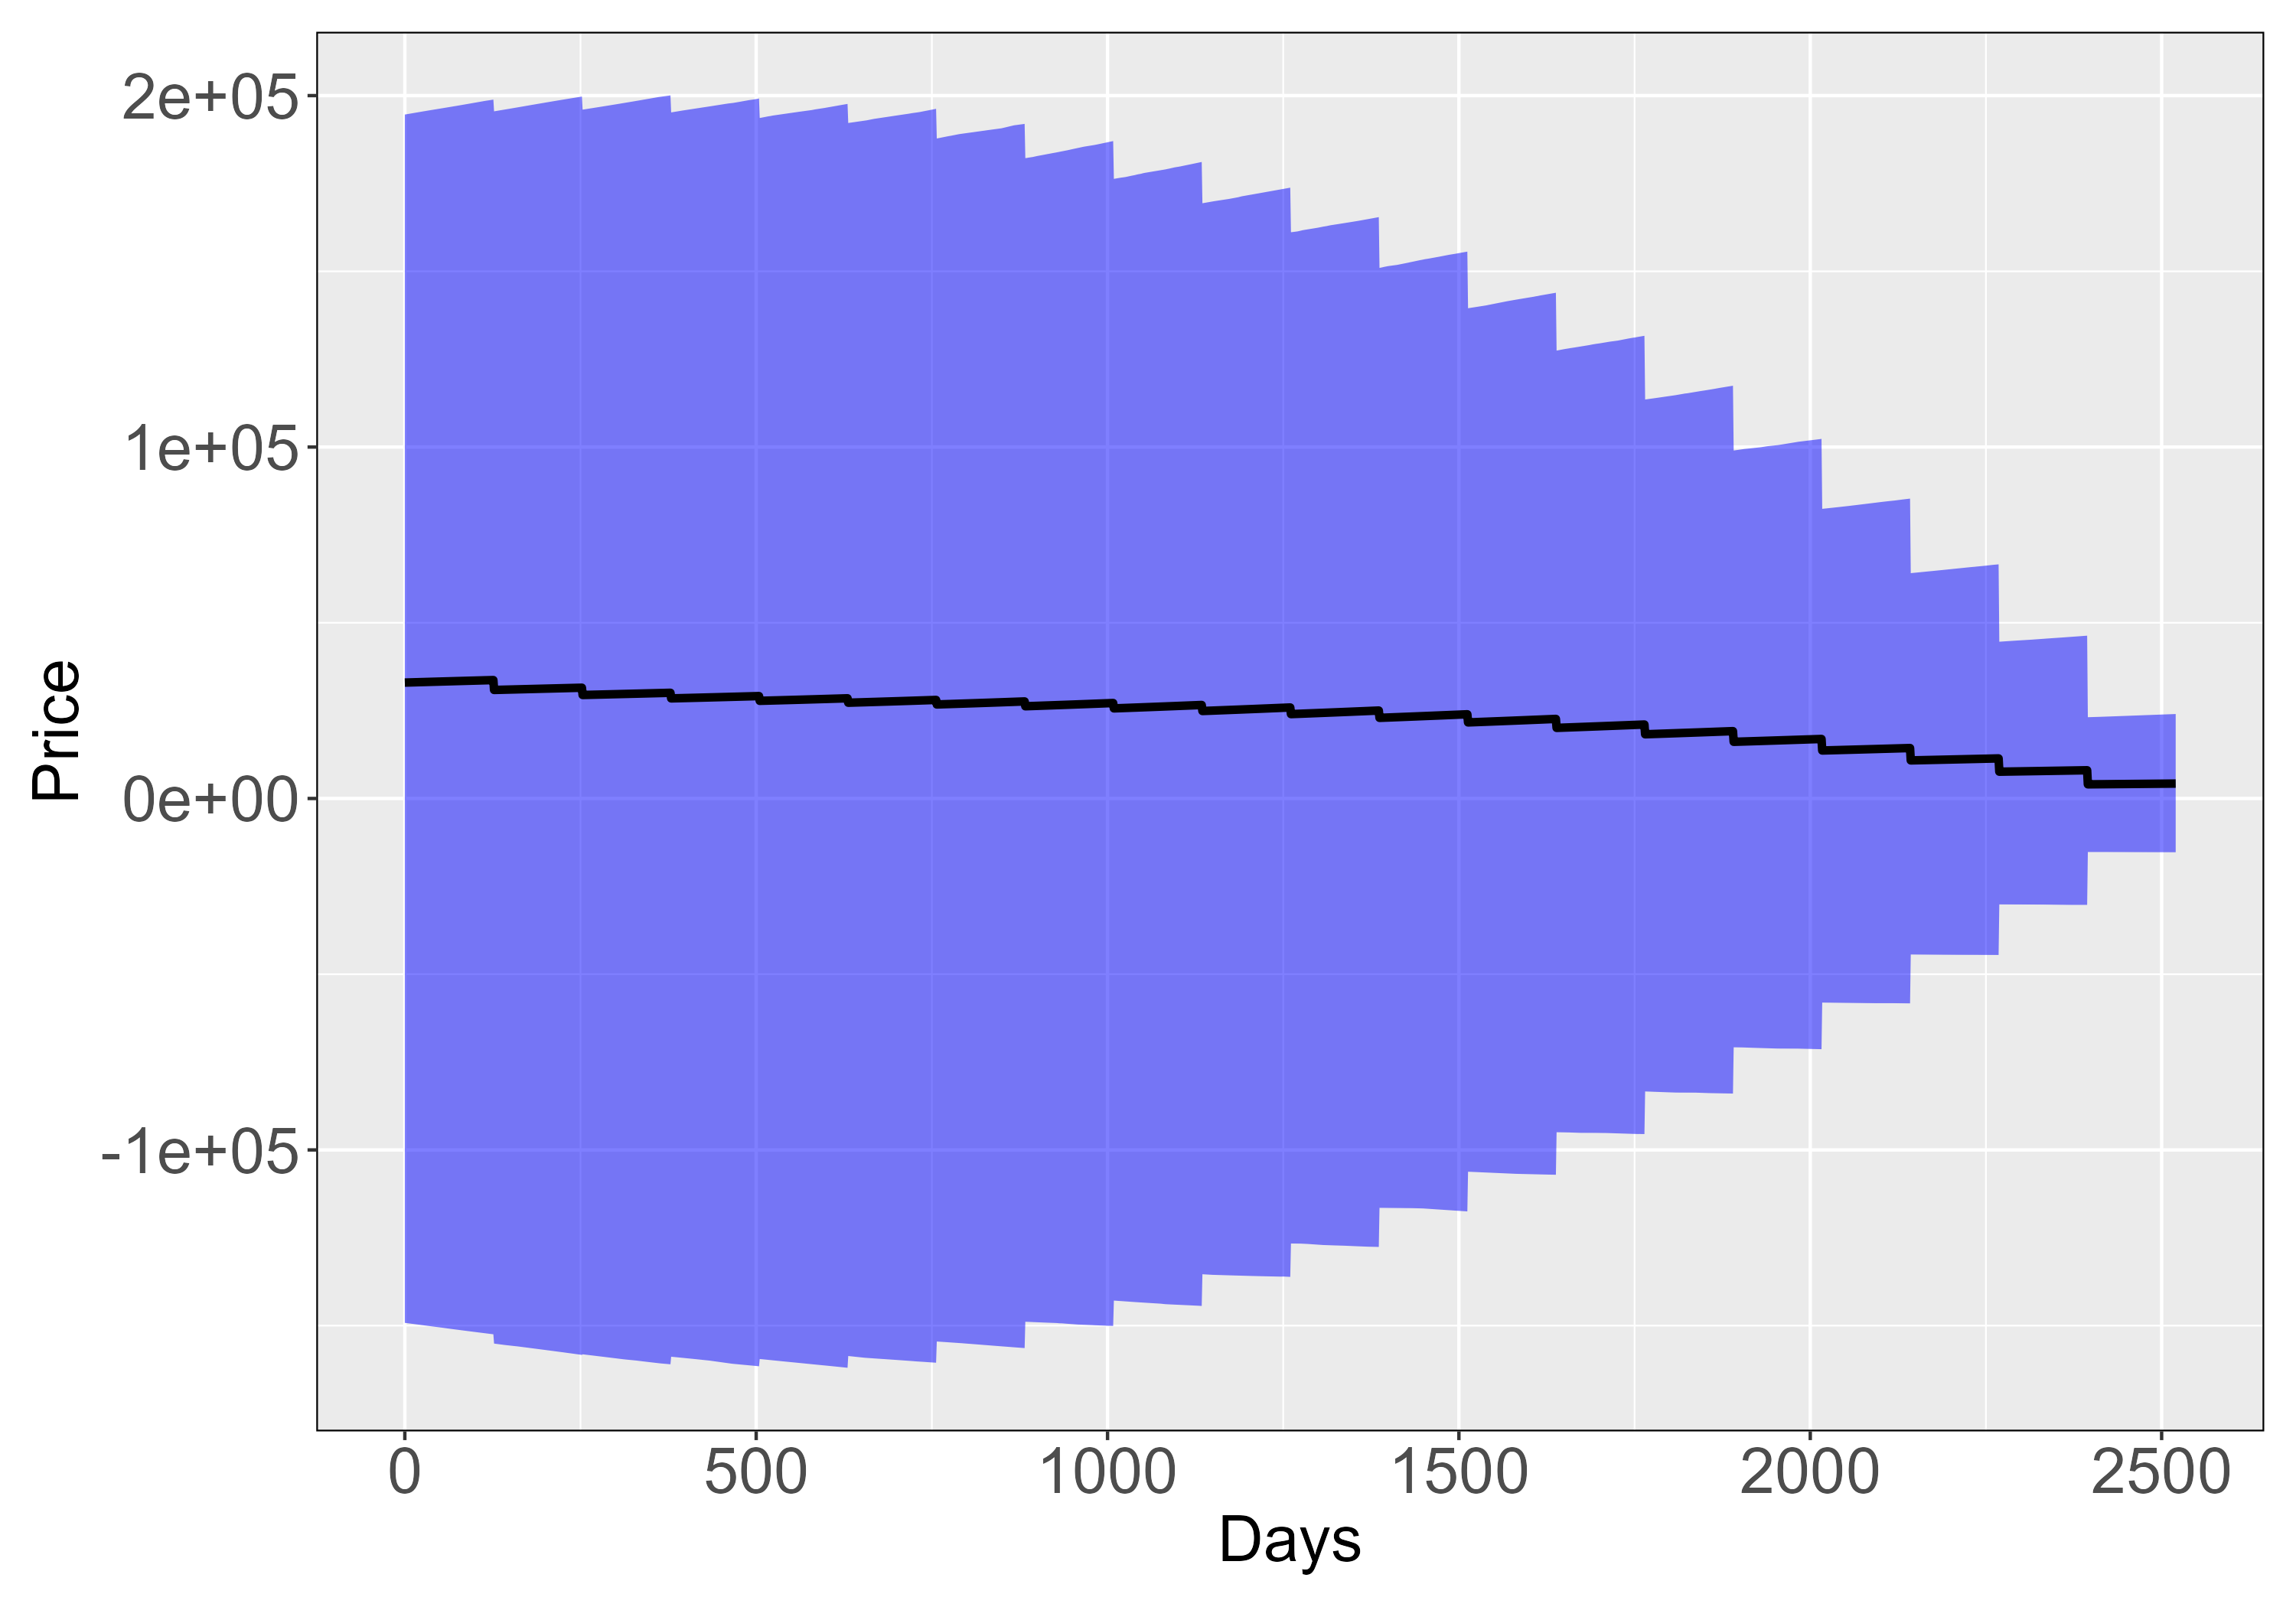
\includegraphics[width=\textwidth]{Figures/Prices/procedure_2_spline_model_prices_plot.png}
        \subcaption{Spline model using procedure 2.}
        \label{fig:irs of procedure 2, spline.}
    \end{subfigure}
    \caption[The price of swaps from the four different models.]{The price of swaps from the four different models. The \textbf{black} $\bigl($\textbf{---}$\bigr)$ line is the expected value of the swaps, and the \textbf{shaded blue} $\bigl($\textcolor{shaded_blue_}{\textbf{---}}$\bigr)$ area is the $95\%$ prediction interval for the prices. The prices are extremely similar to each other.}
    \label{fig:irs prices}
\end{figure}

\begin{figure}[!htbp]
    \centering
    \captionsetup{type=figure}
    \begin{subfigure}{0.49\textwidth}
        \centering
        \captionsetup{justification=centering}
        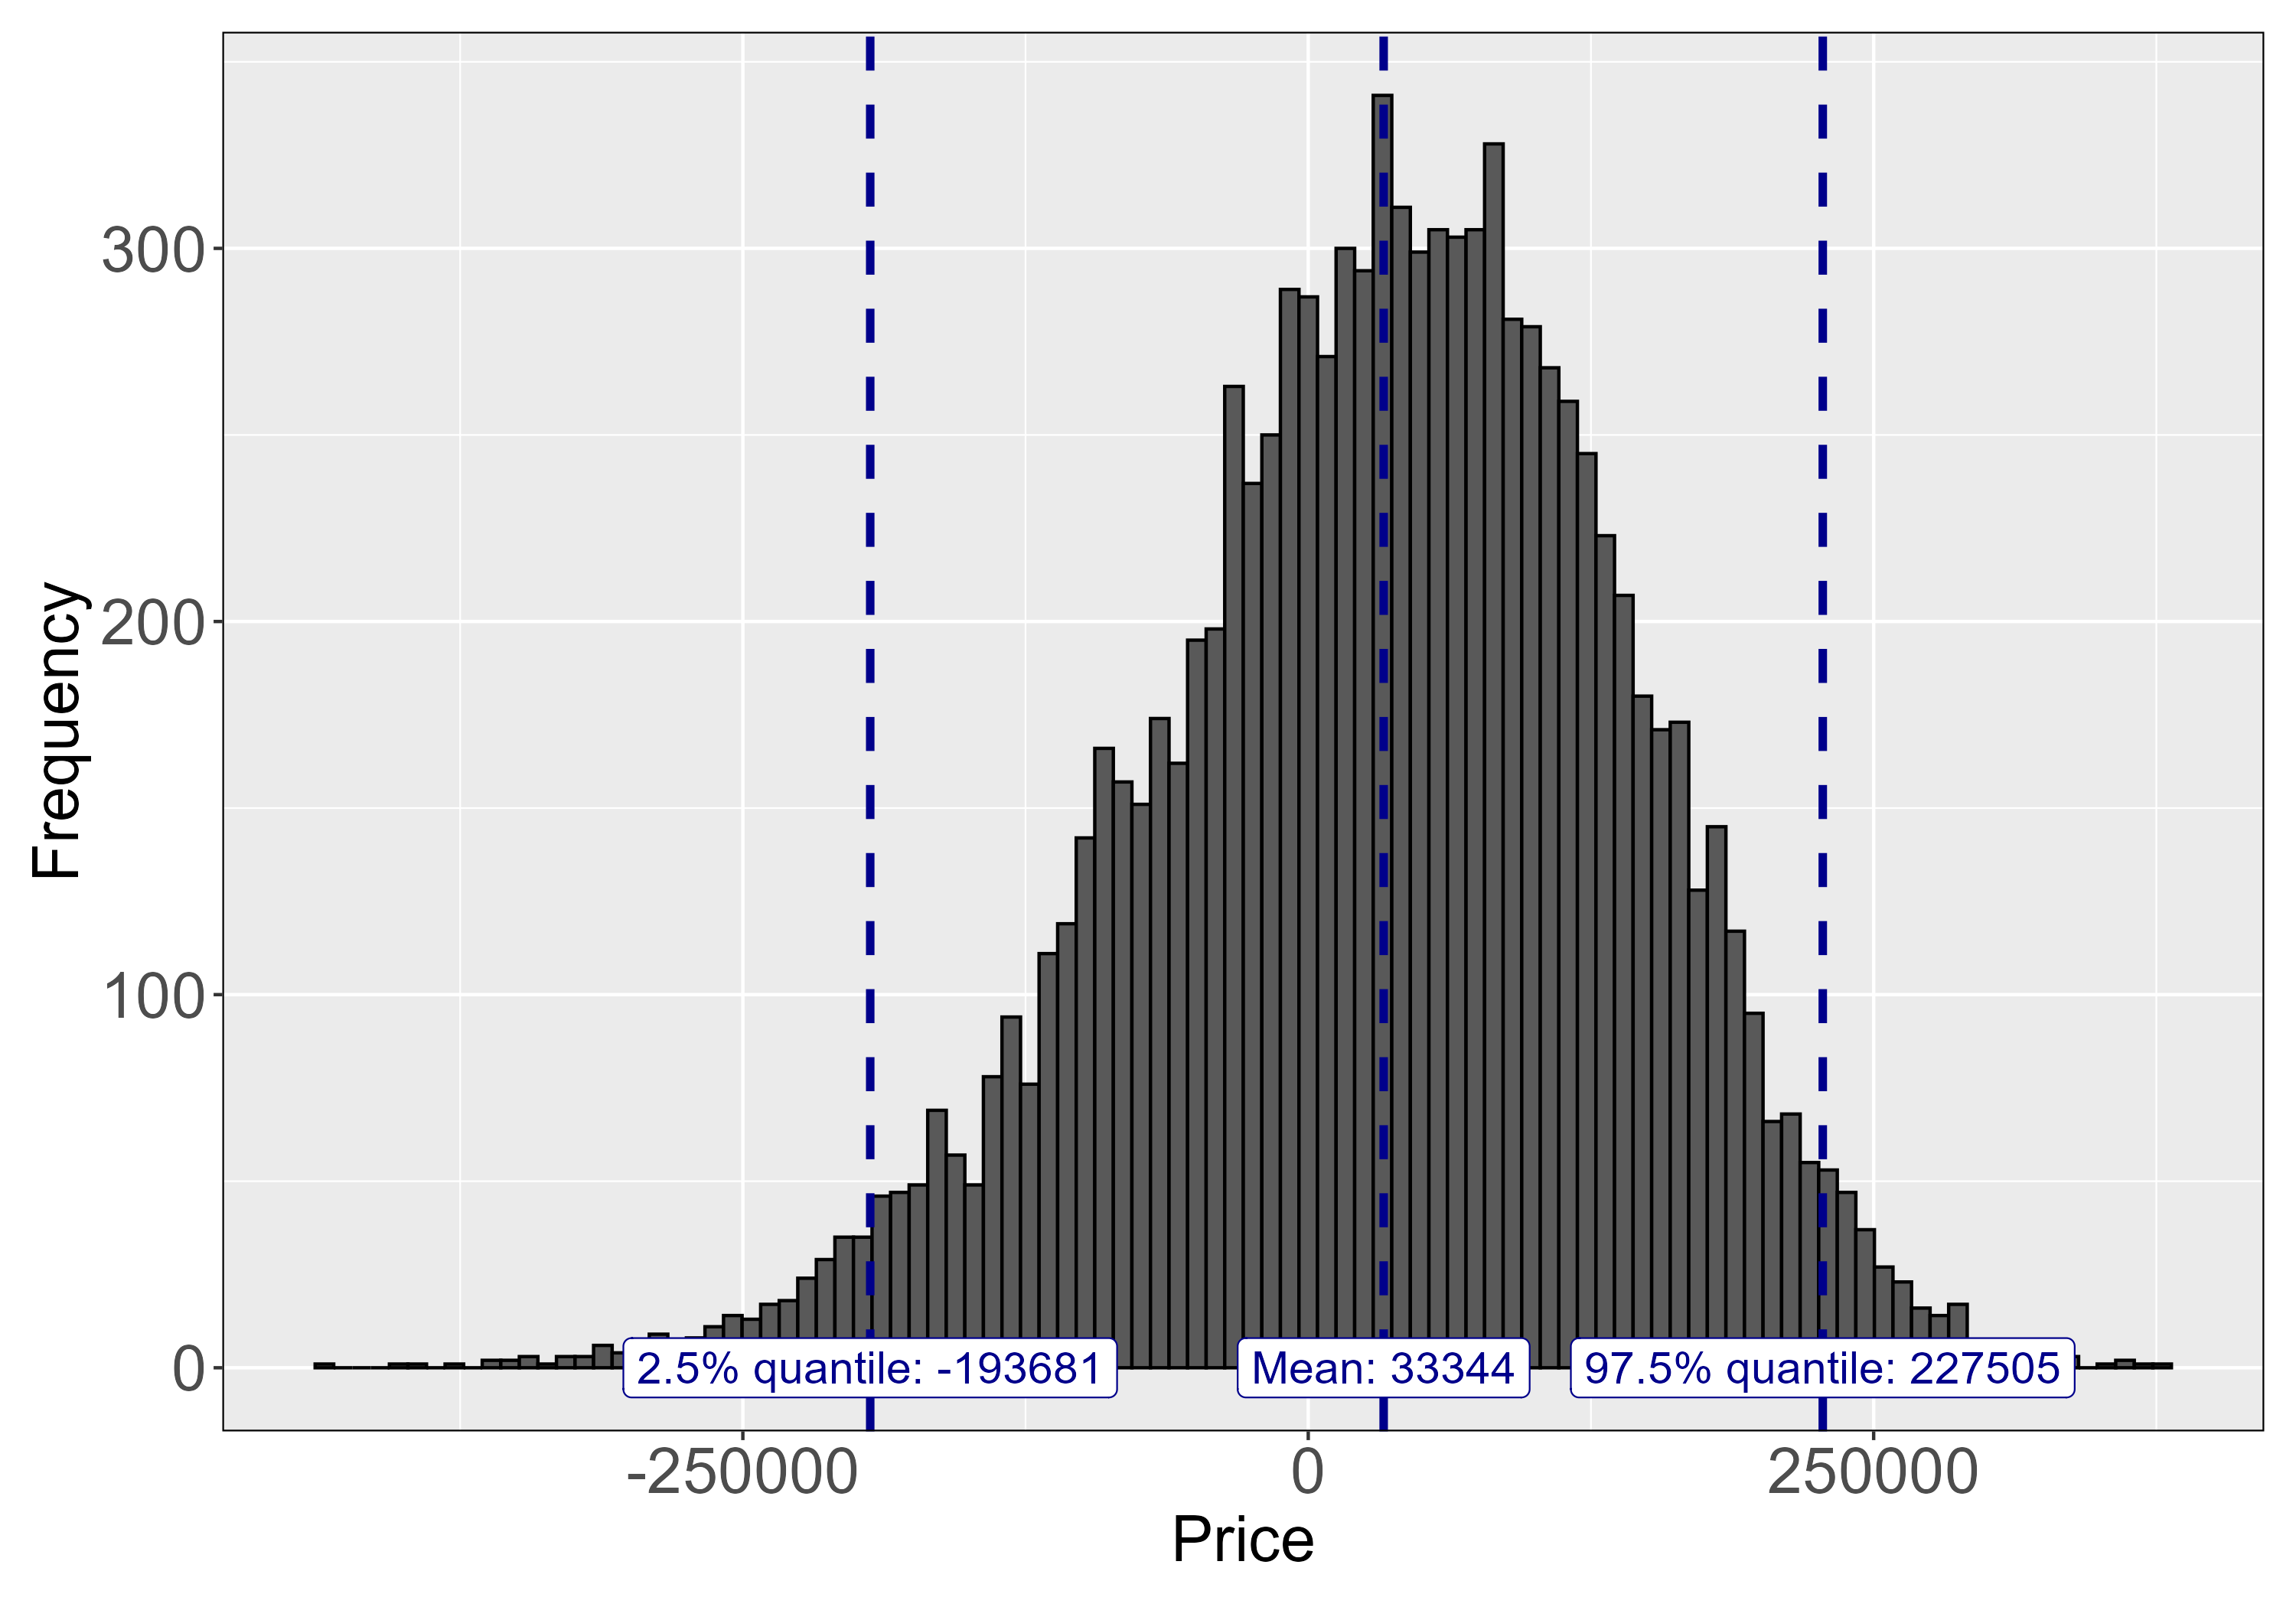
\includegraphics[width=\textwidth]{Figures/Prices/procedure_1_poly_model_histogram.png}
        \subcaption{Polynomial model using procedure 1.}
        \label{fig:irs hist of procedure 1, poly.}
    \end{subfigure}
    \hfill
    \begin{subfigure}{0.49\textwidth}
        \centering
        \captionsetup{justification=centering}
        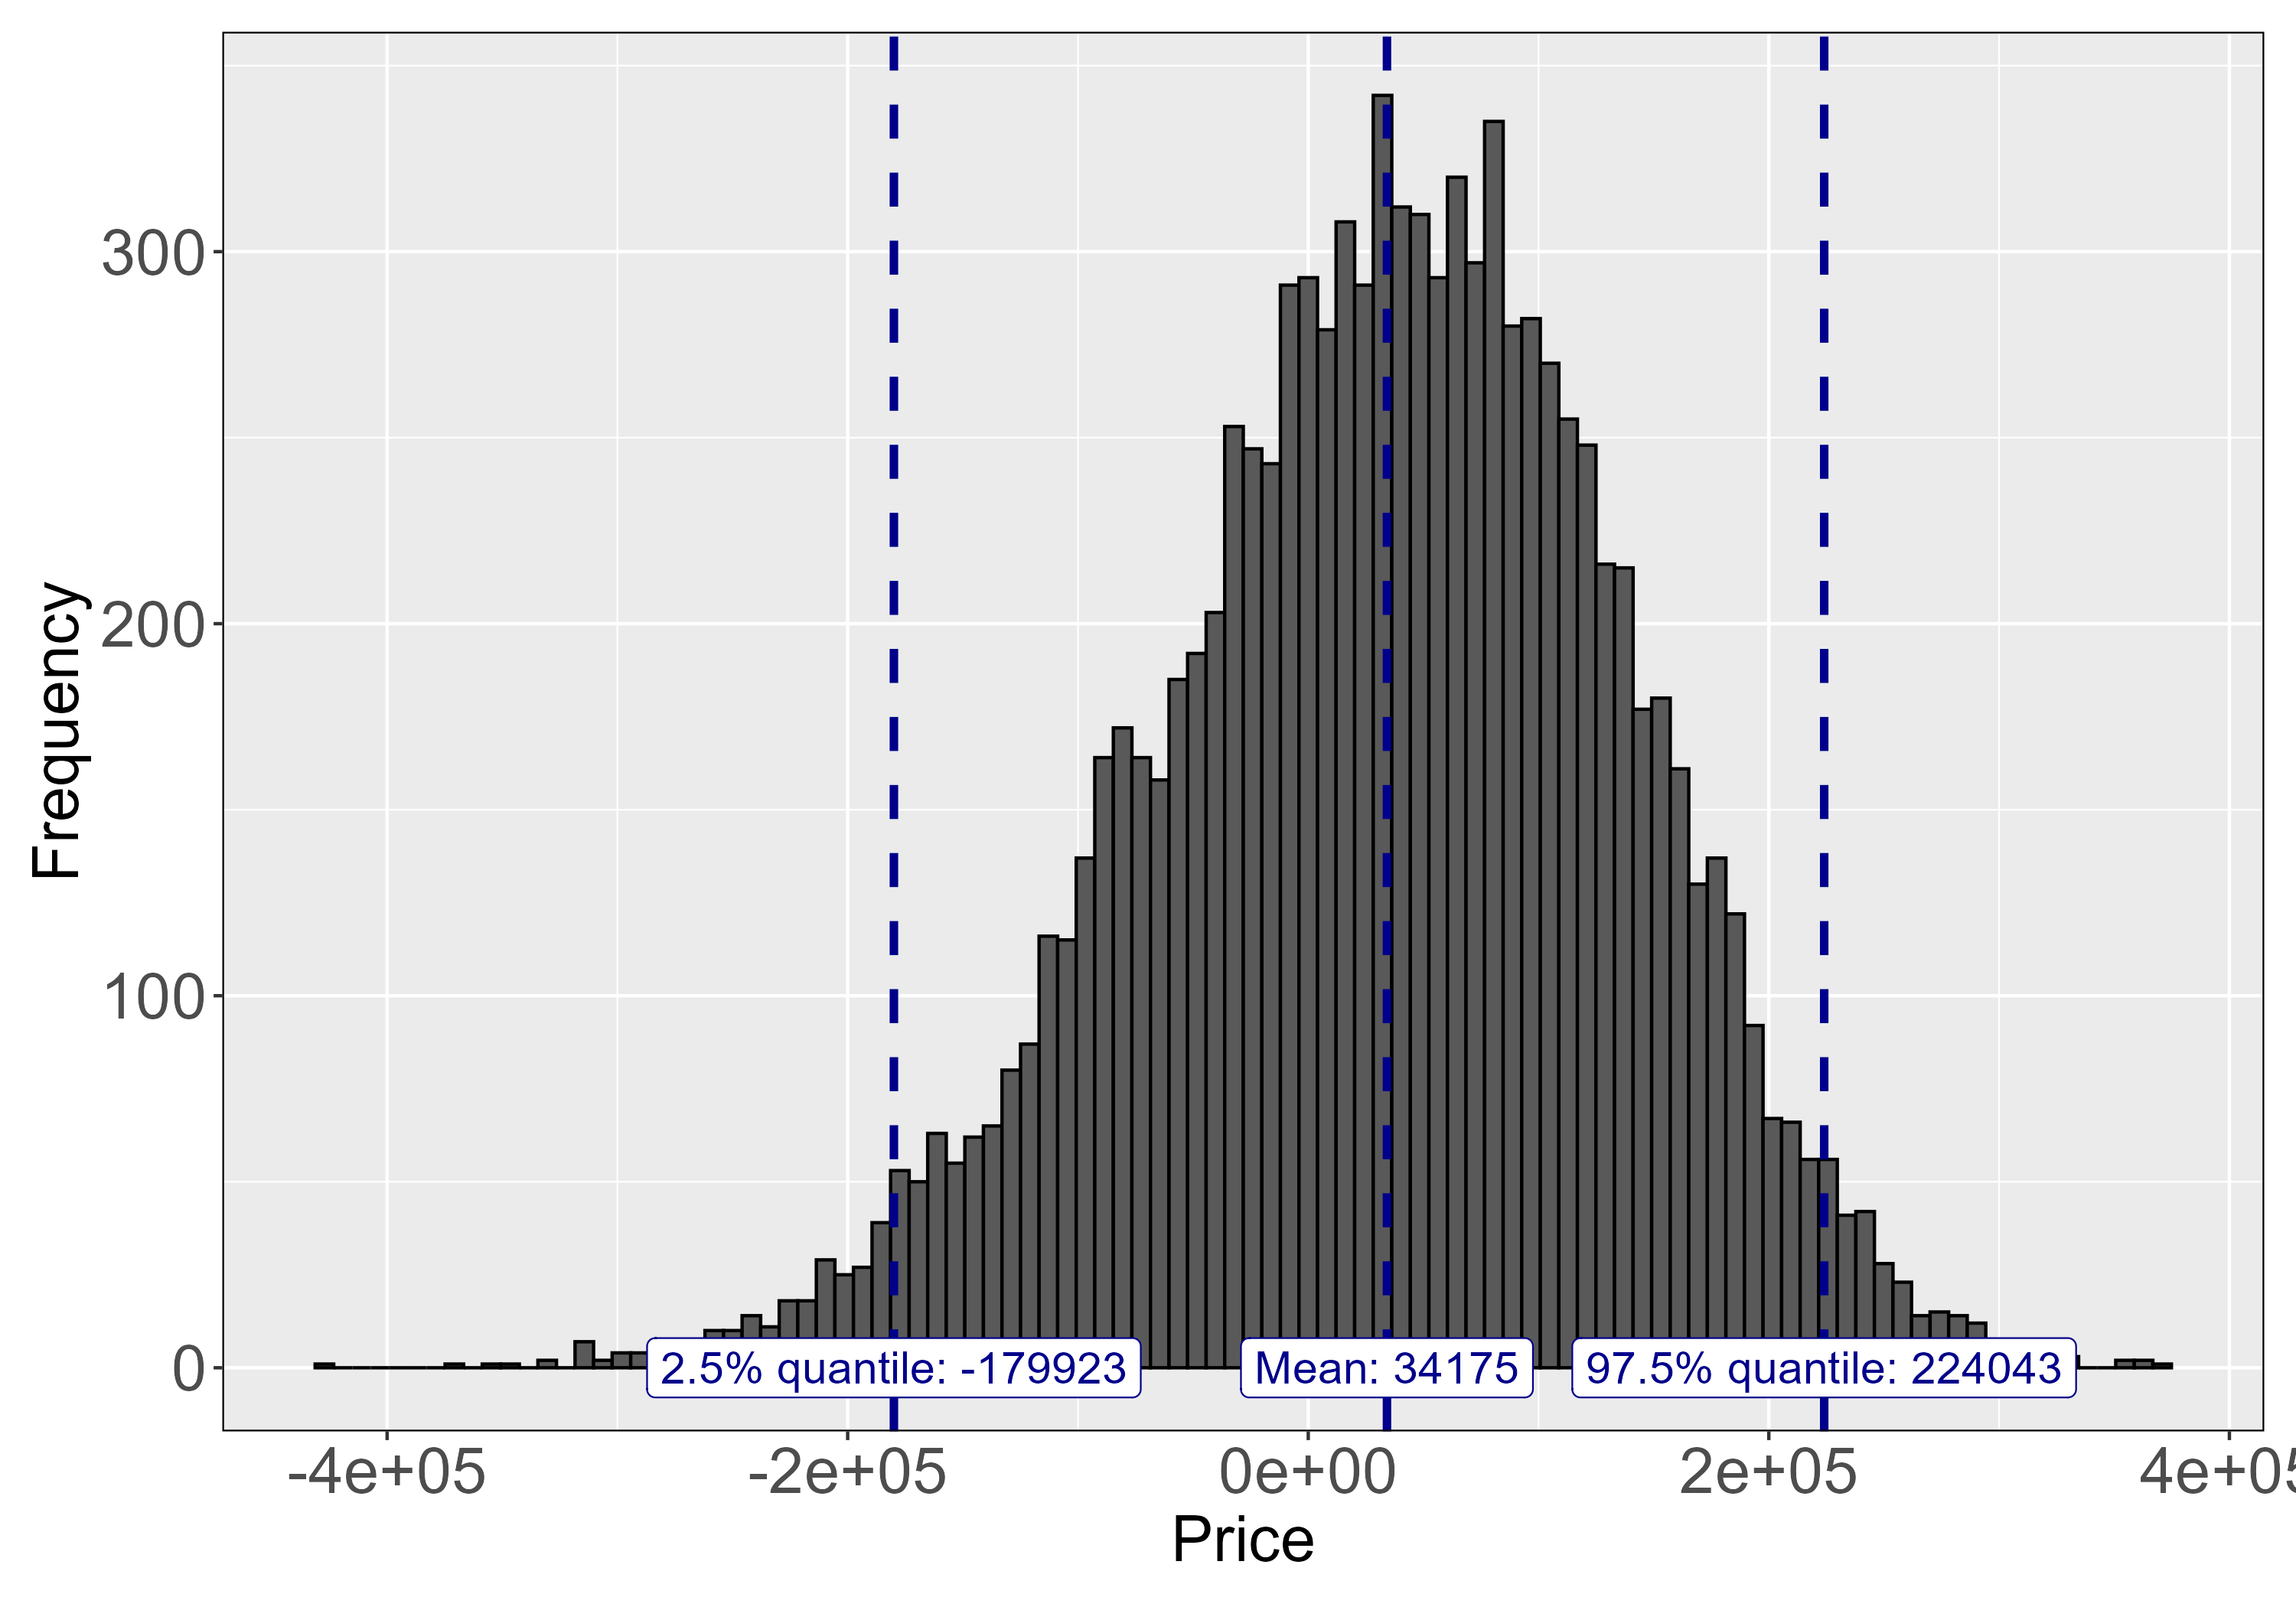
\includegraphics[width=\textwidth]{Figures/Prices/procedure_1_spline_model_histogram.png}
        \subcaption{Spline model using procedure 1.}
        \label{fig:irs hist of procedure 1, spline.}
    \end{subfigure}
    \vskip\baselineskip
    \begin{subfigure}{0.49\textwidth}
        \centering
        \captionsetup{justification=centering}
        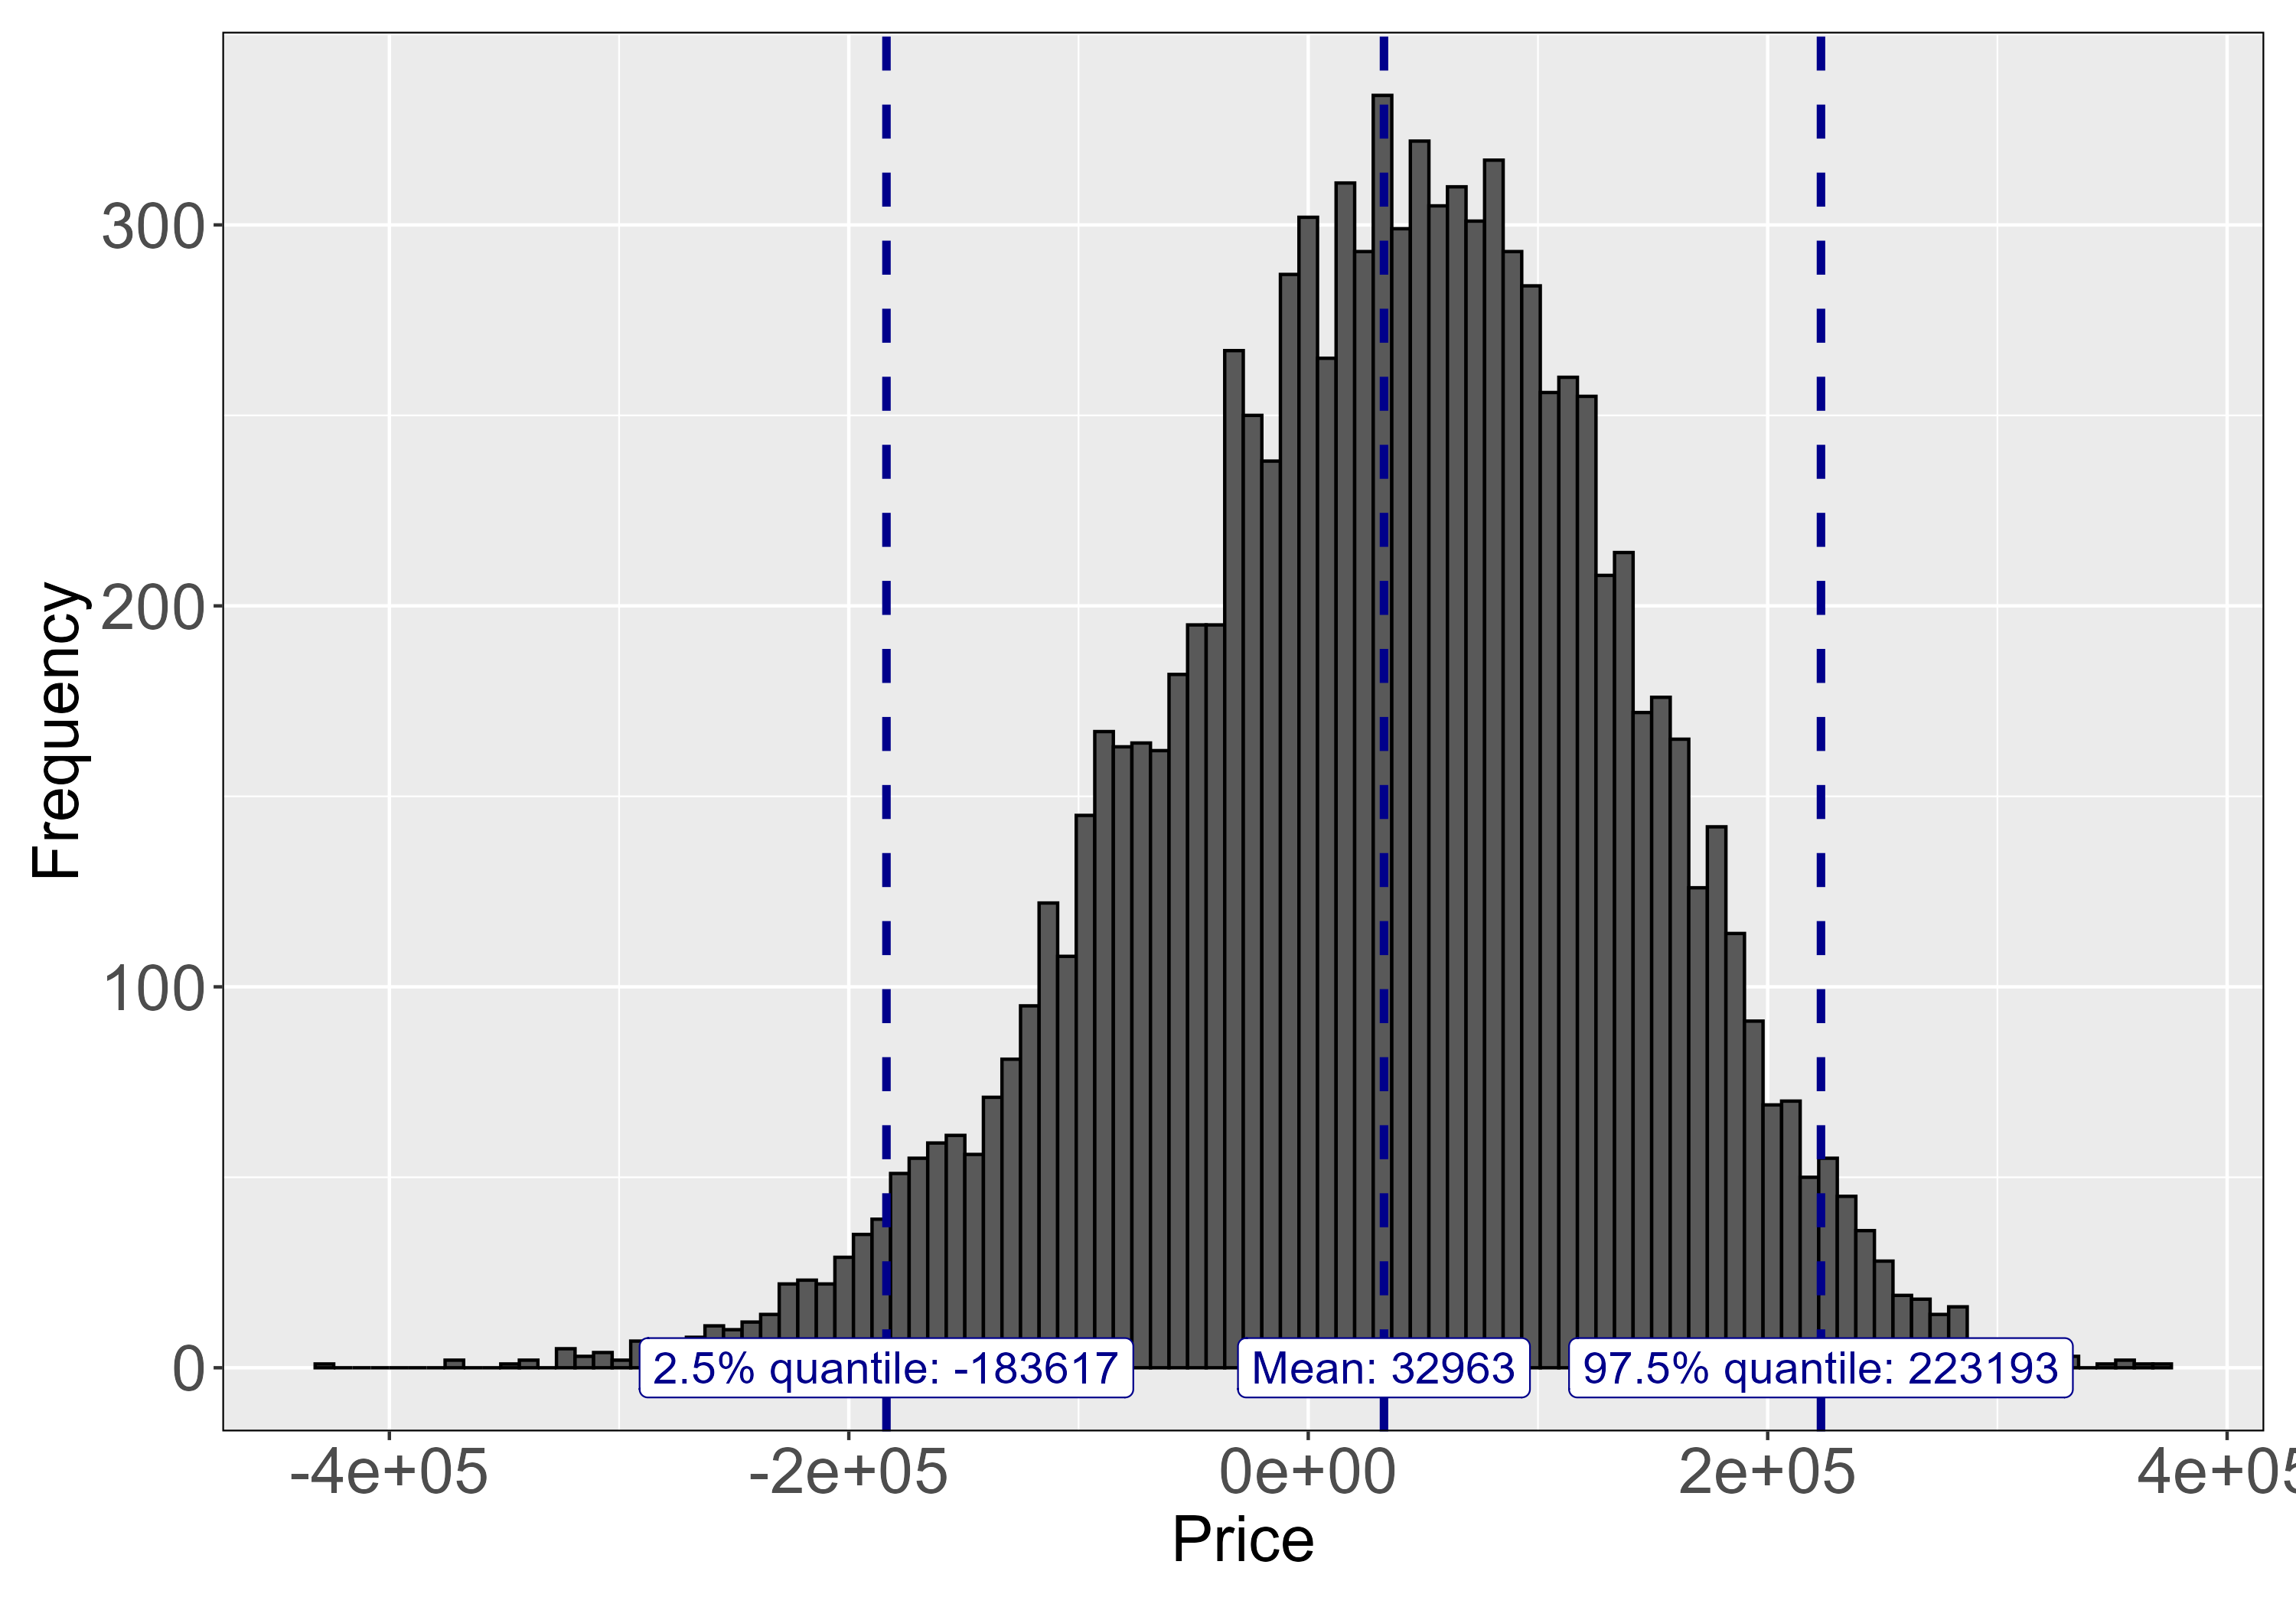
\includegraphics[width=\textwidth]{Figures/Prices/procedure_2_poly_model_histogram.png}
        \subcaption{Polynomial model using procedure 2.}
        \label{fig:irs hist of procedure 2, poly.}
    \end{subfigure}
    \hfill
    \begin{subfigure}{0.49\textwidth}
        \centering
        \captionsetup{justification=centering}
        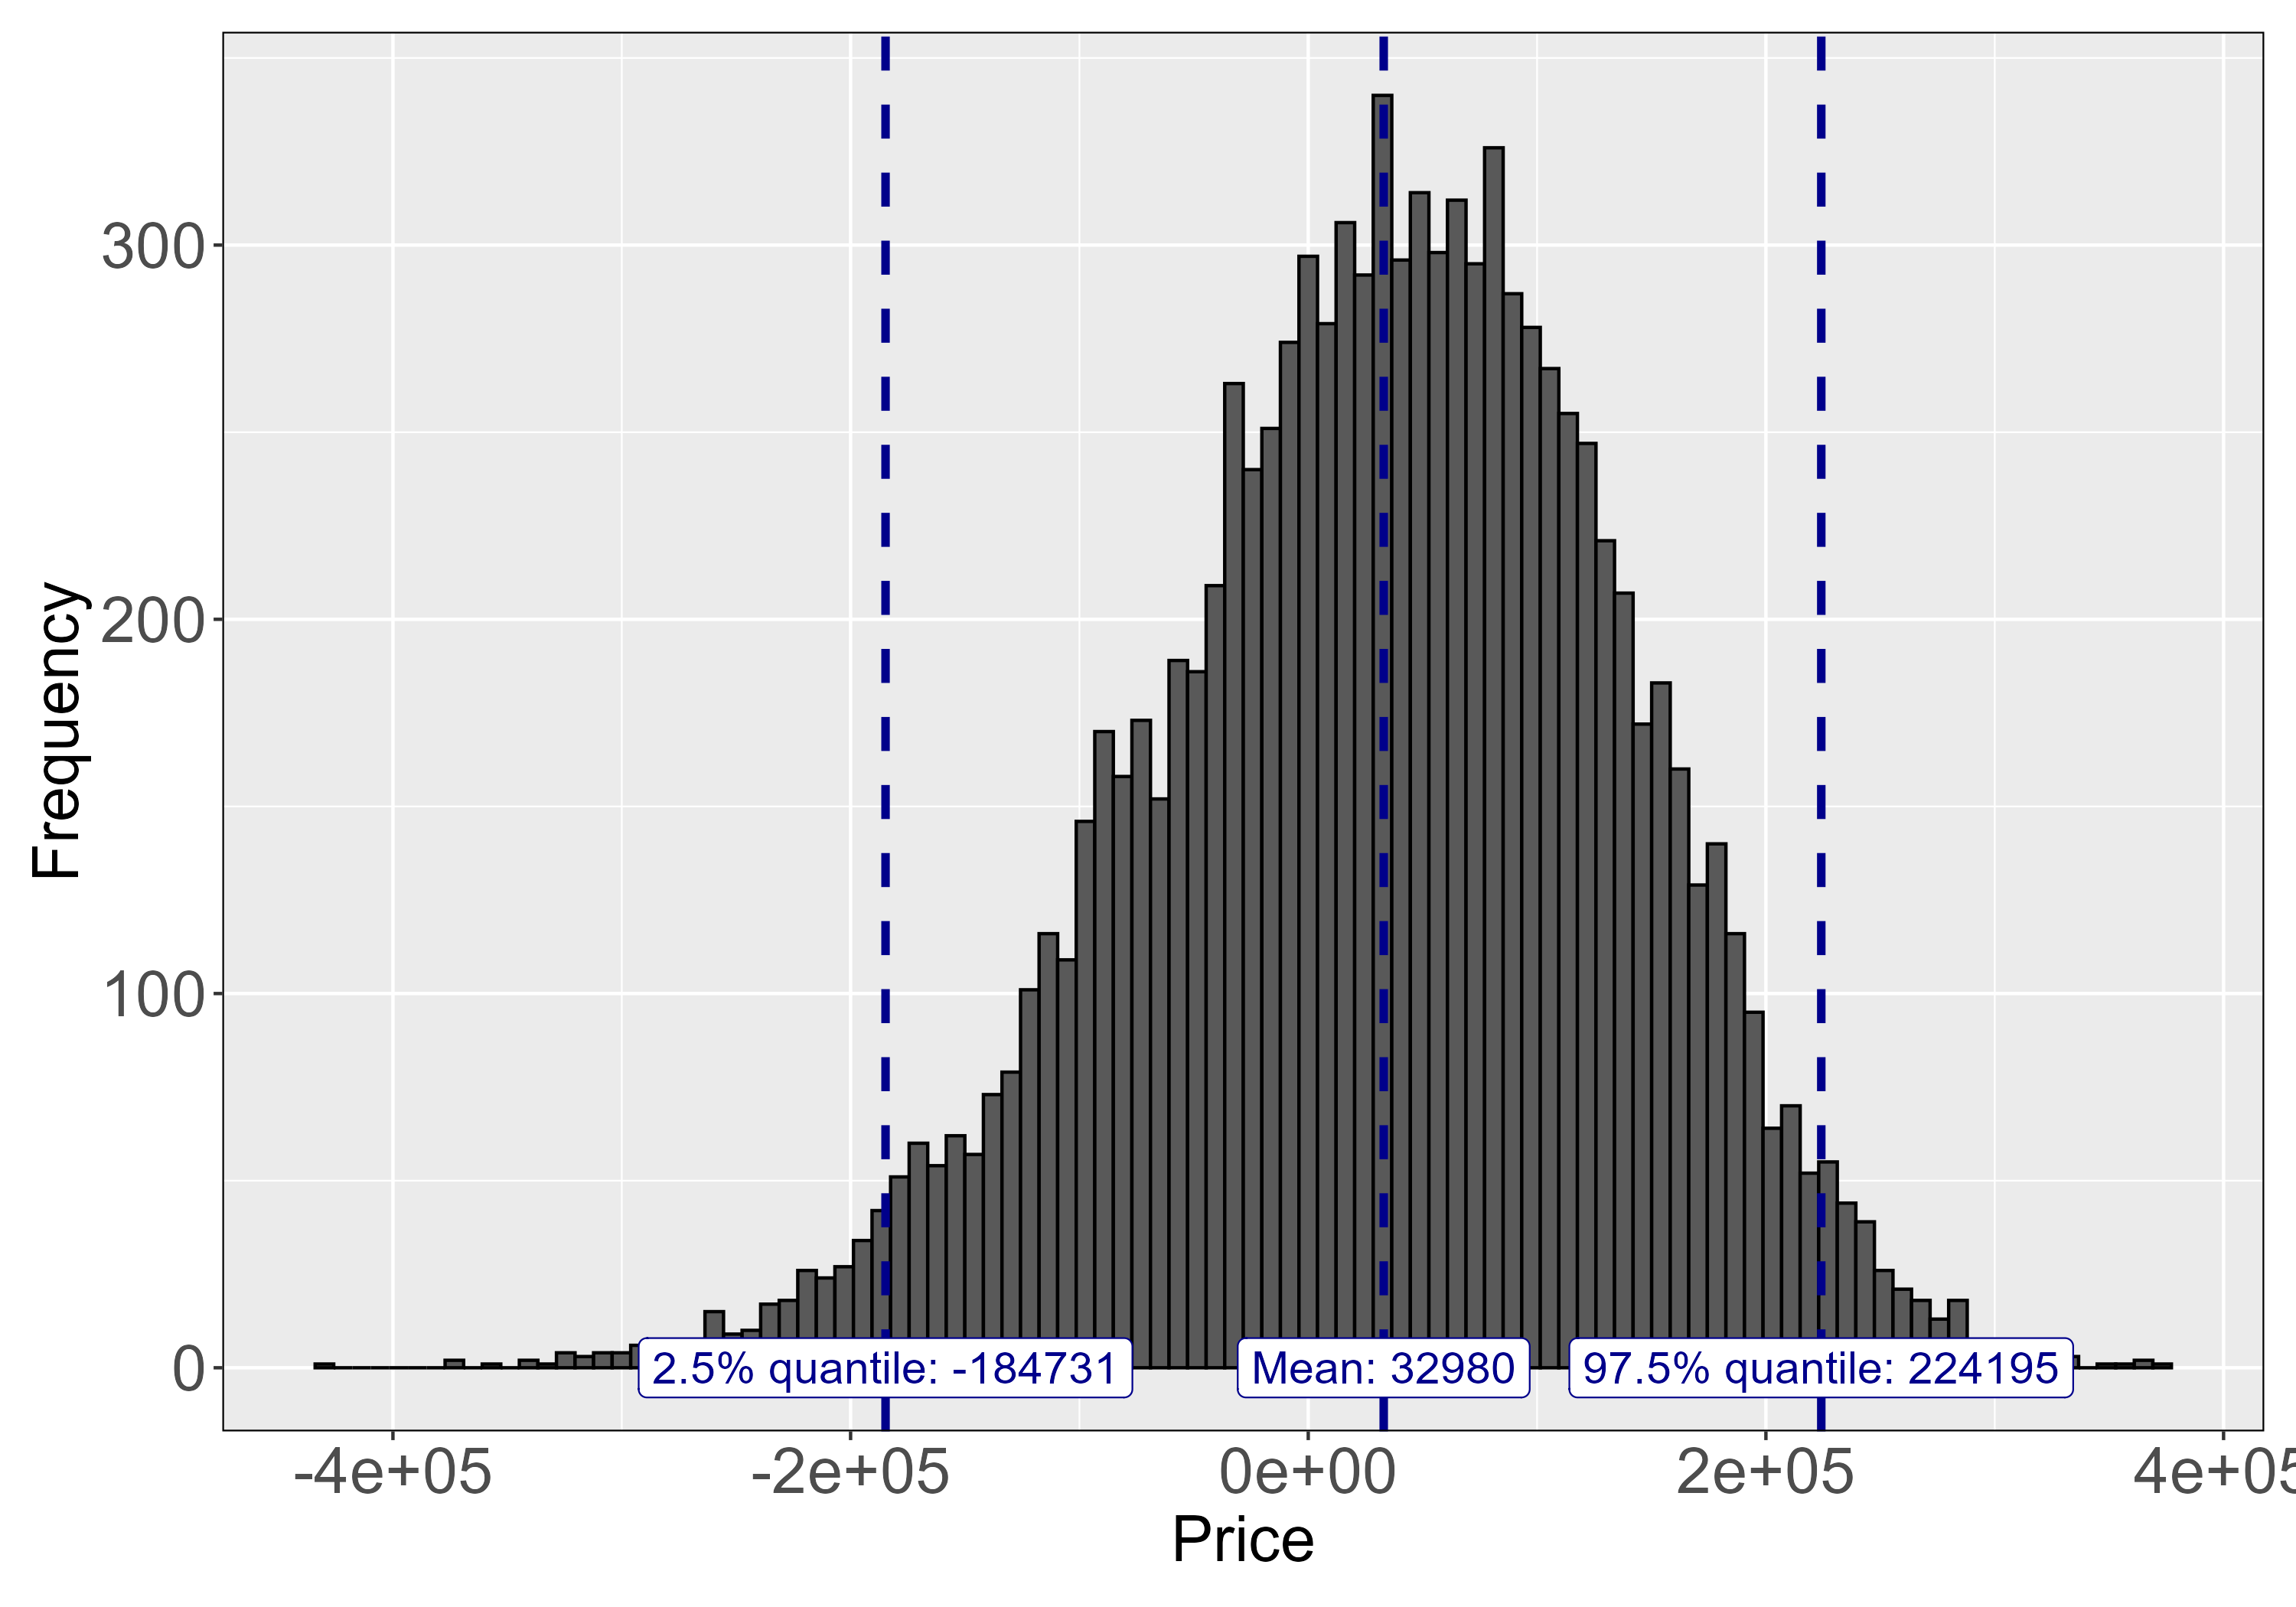
\includegraphics[width=\textwidth]{Figures/Prices/procedure_2_spline_model_histogram.png}
        \subcaption{Spline model using procedure 2.}
        \label{fig:irs hist of procedure 2, spline.}
    \end{subfigure}
    \caption[The histogram of the swap prices today generated by the four different models.]{The histogram of the swap prices today generated by the four different models. The models from procedure 2 give identical results, while the models from procedure 1 have slightly different values.}
    \label{fig:irs prices hist today}
\end{figure}

\begin{figure}[!htbp]
    \centering
    \captionsetup{type=figure}
    \begin{subfigure}{0.49\textwidth}
        \centering
        \captionsetup{justification=centering}
        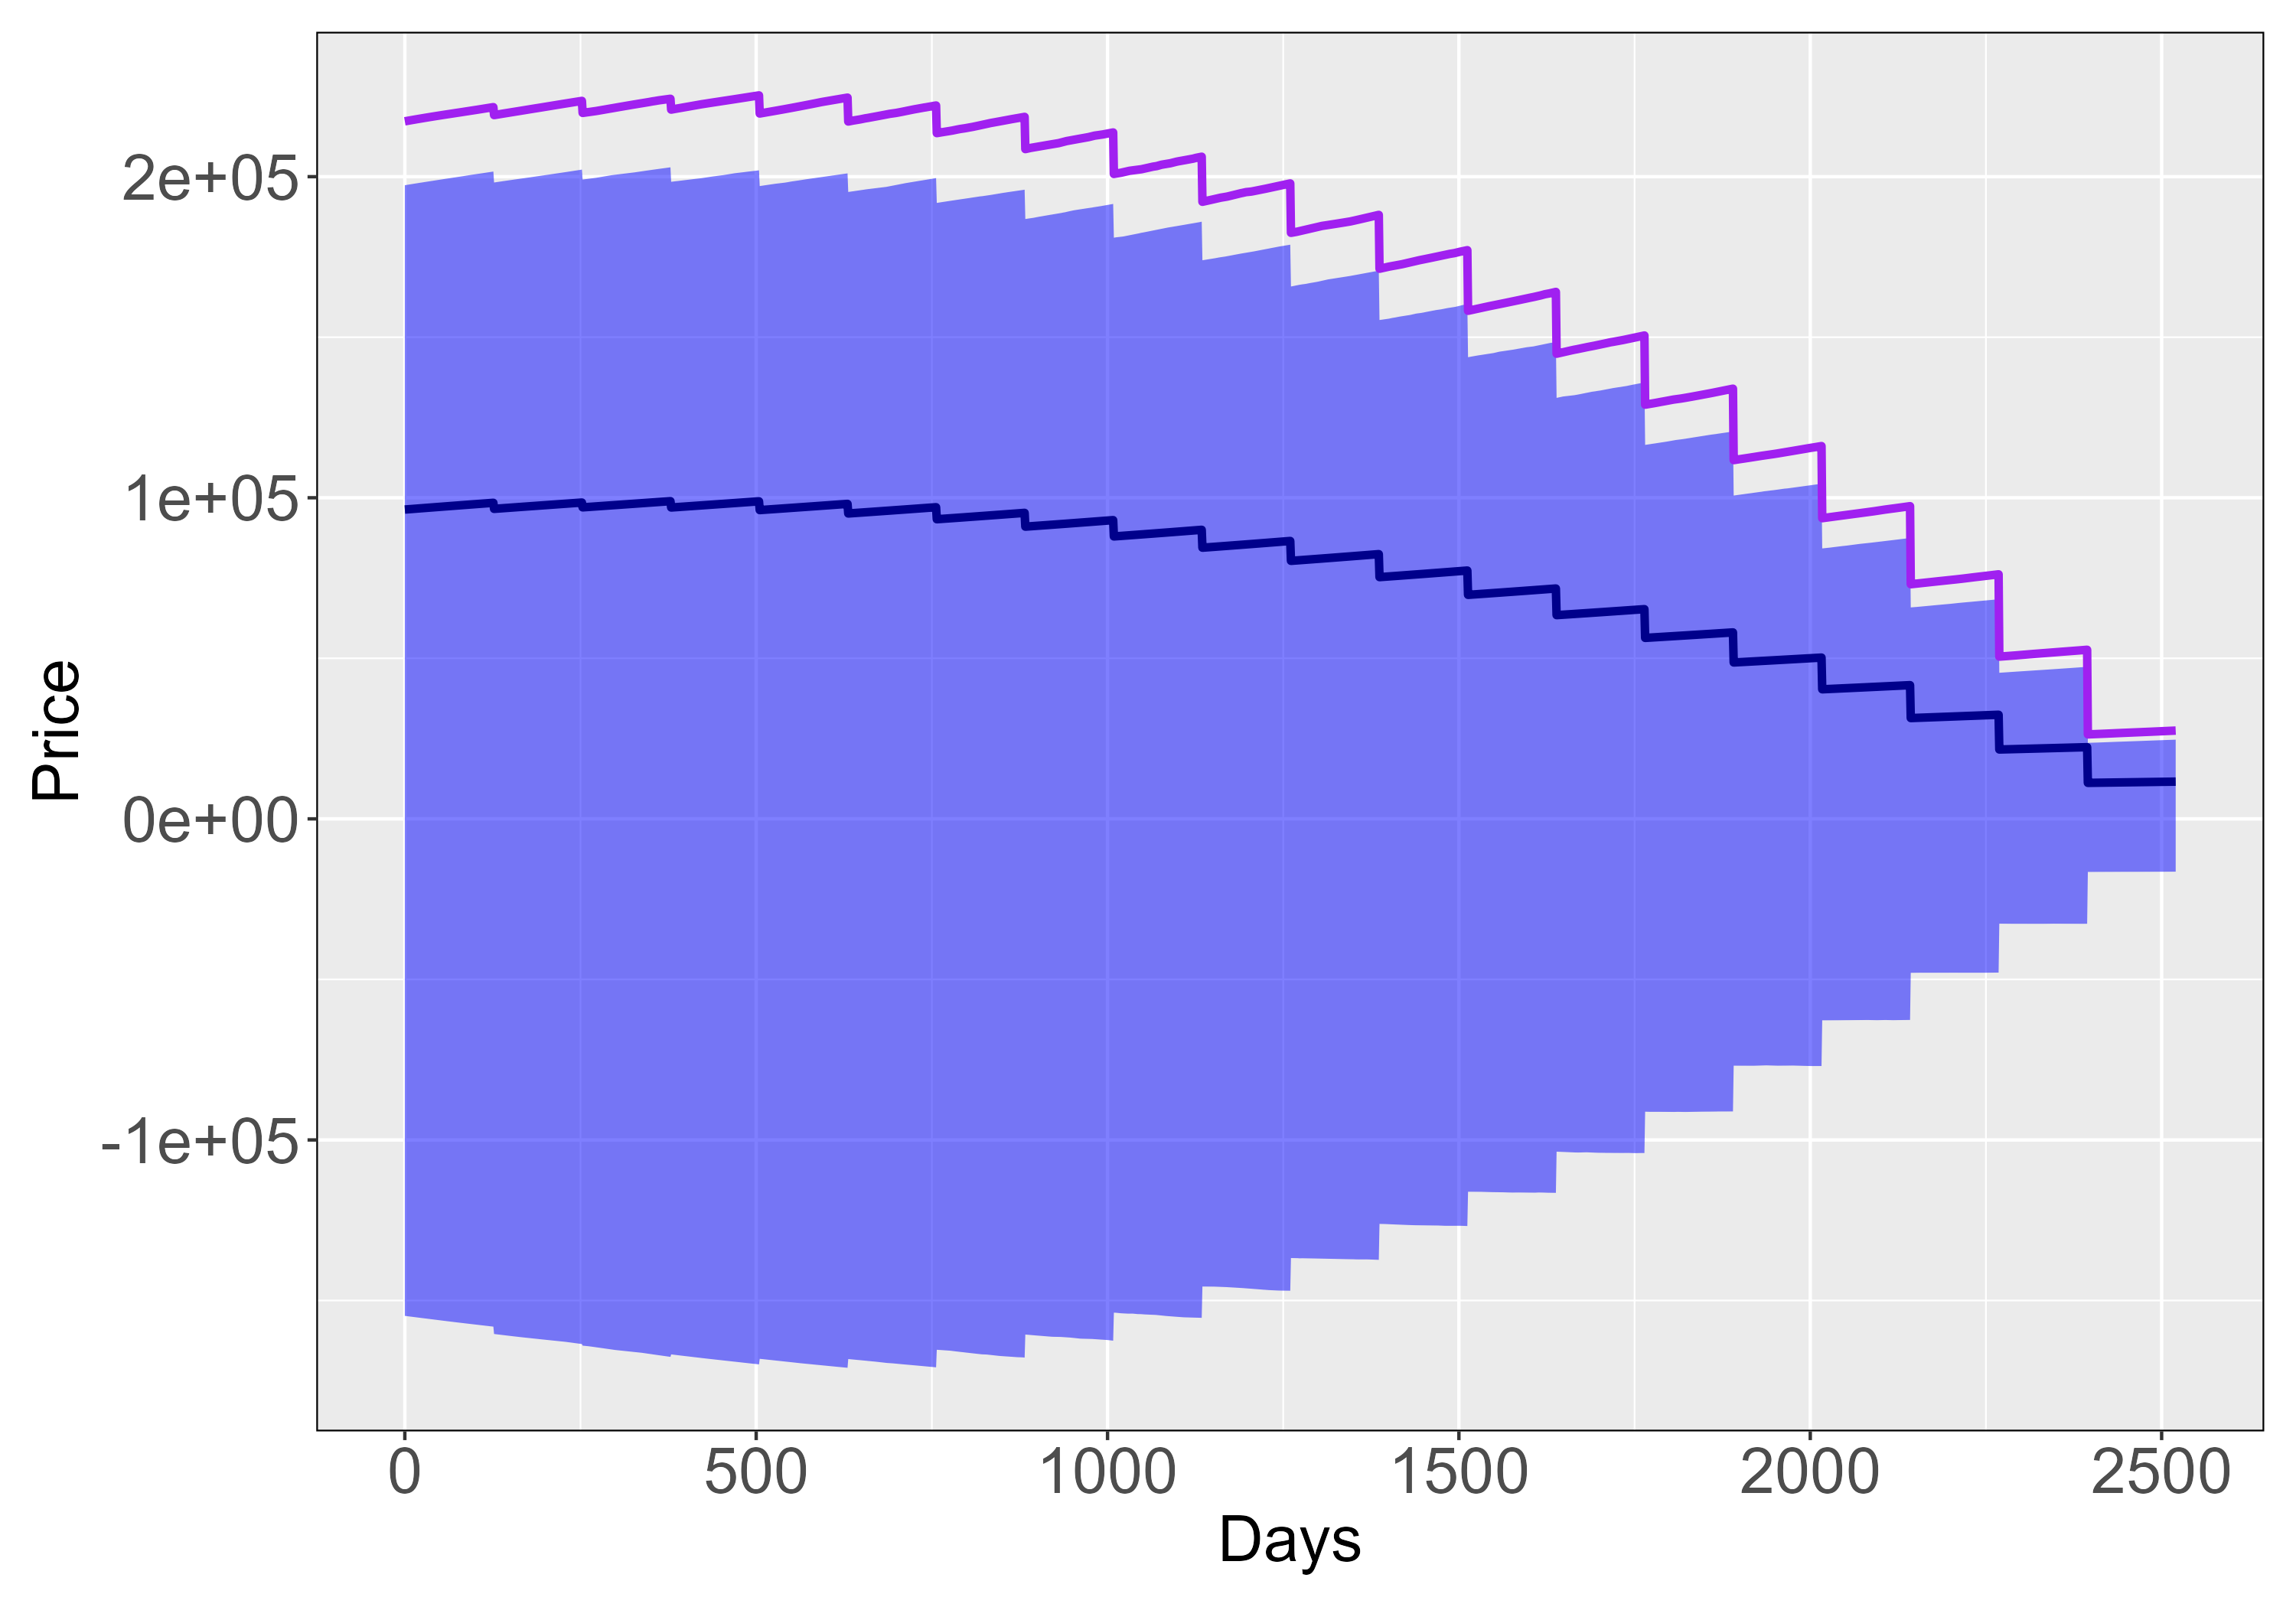
\includegraphics[width=\textwidth]{Figures/Exposure/procedure_1_poly_model_exposure_plot.png}
        \subcaption{Polynomial model using procedure 1.}
        \label{fig:exposure of procedure 1, poly.}
    \end{subfigure}
    \hfill
    \begin{subfigure}{0.49\textwidth}
        \centering
        \captionsetup{justification=centering}
        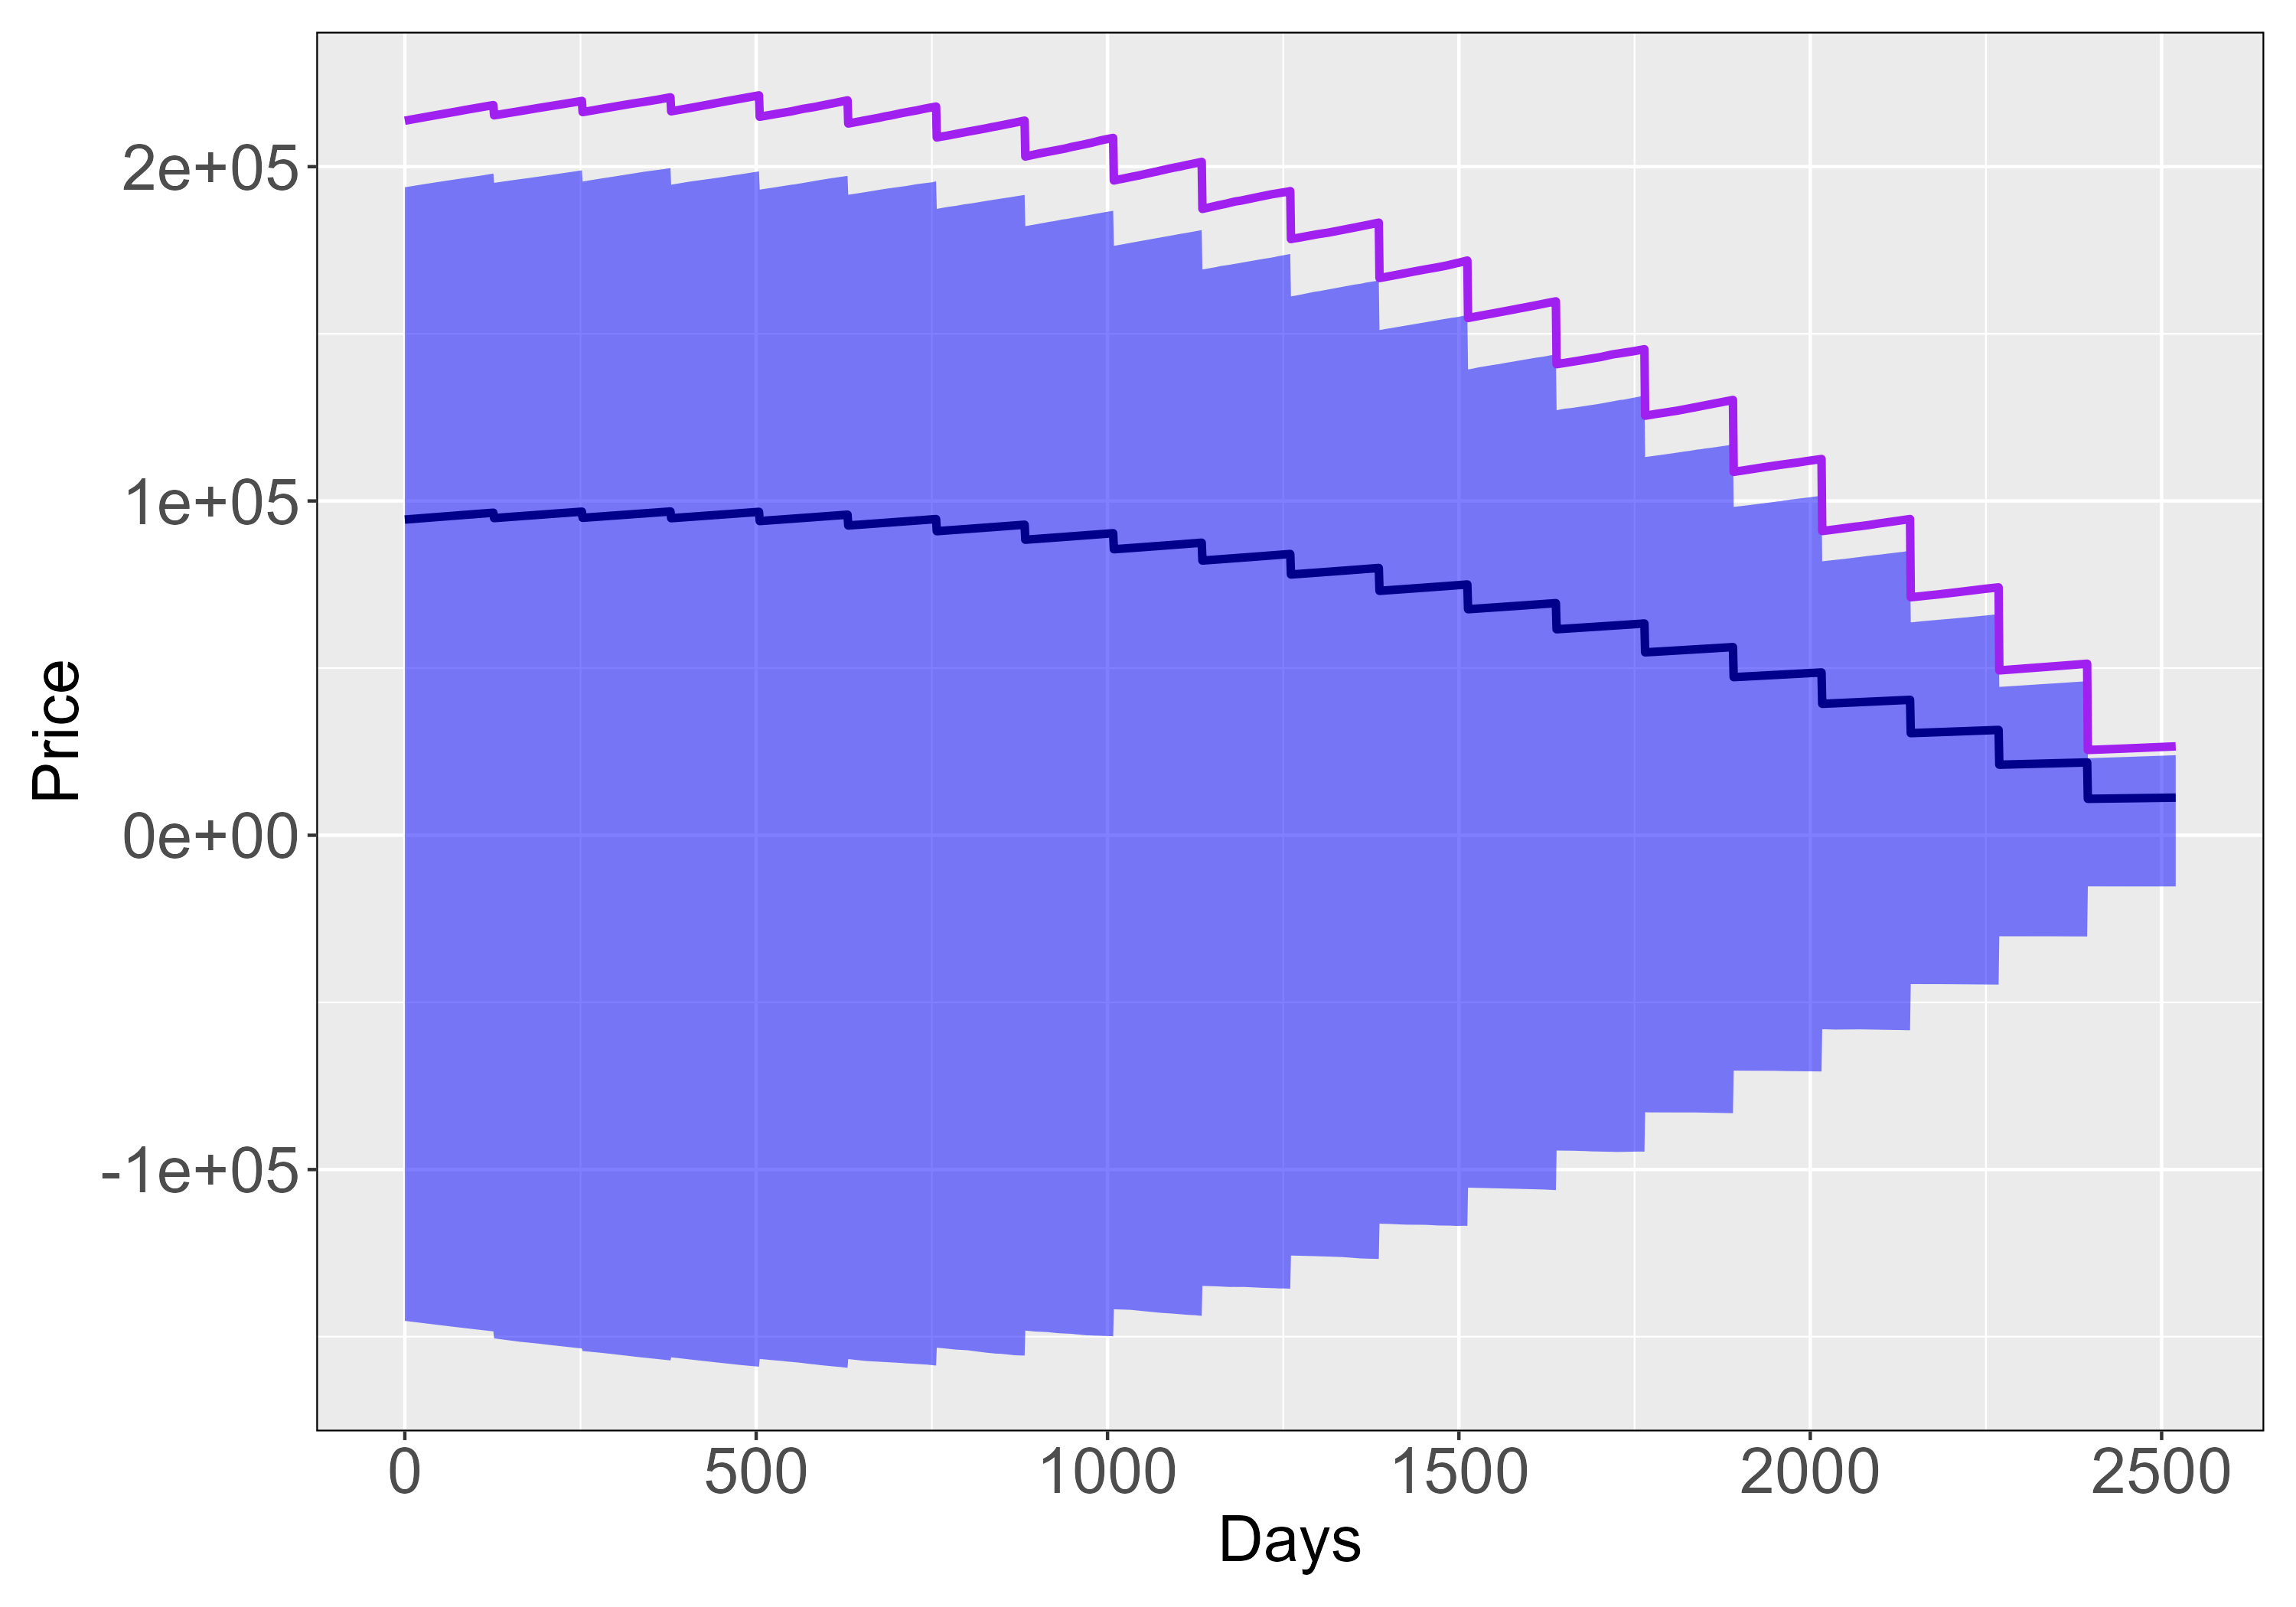
\includegraphics[width=\textwidth]{Figures/Exposure/procedure_1_spline_model_exposure_plot.png}
        \subcaption{Spline model using procedure 1.}
        \label{fig:exposure of procedure 1, spline.}
    \end{subfigure}
    \vskip\baselineskip
    \begin{subfigure}{0.49\textwidth}
        \centering
        \captionsetup{justification=centering}
        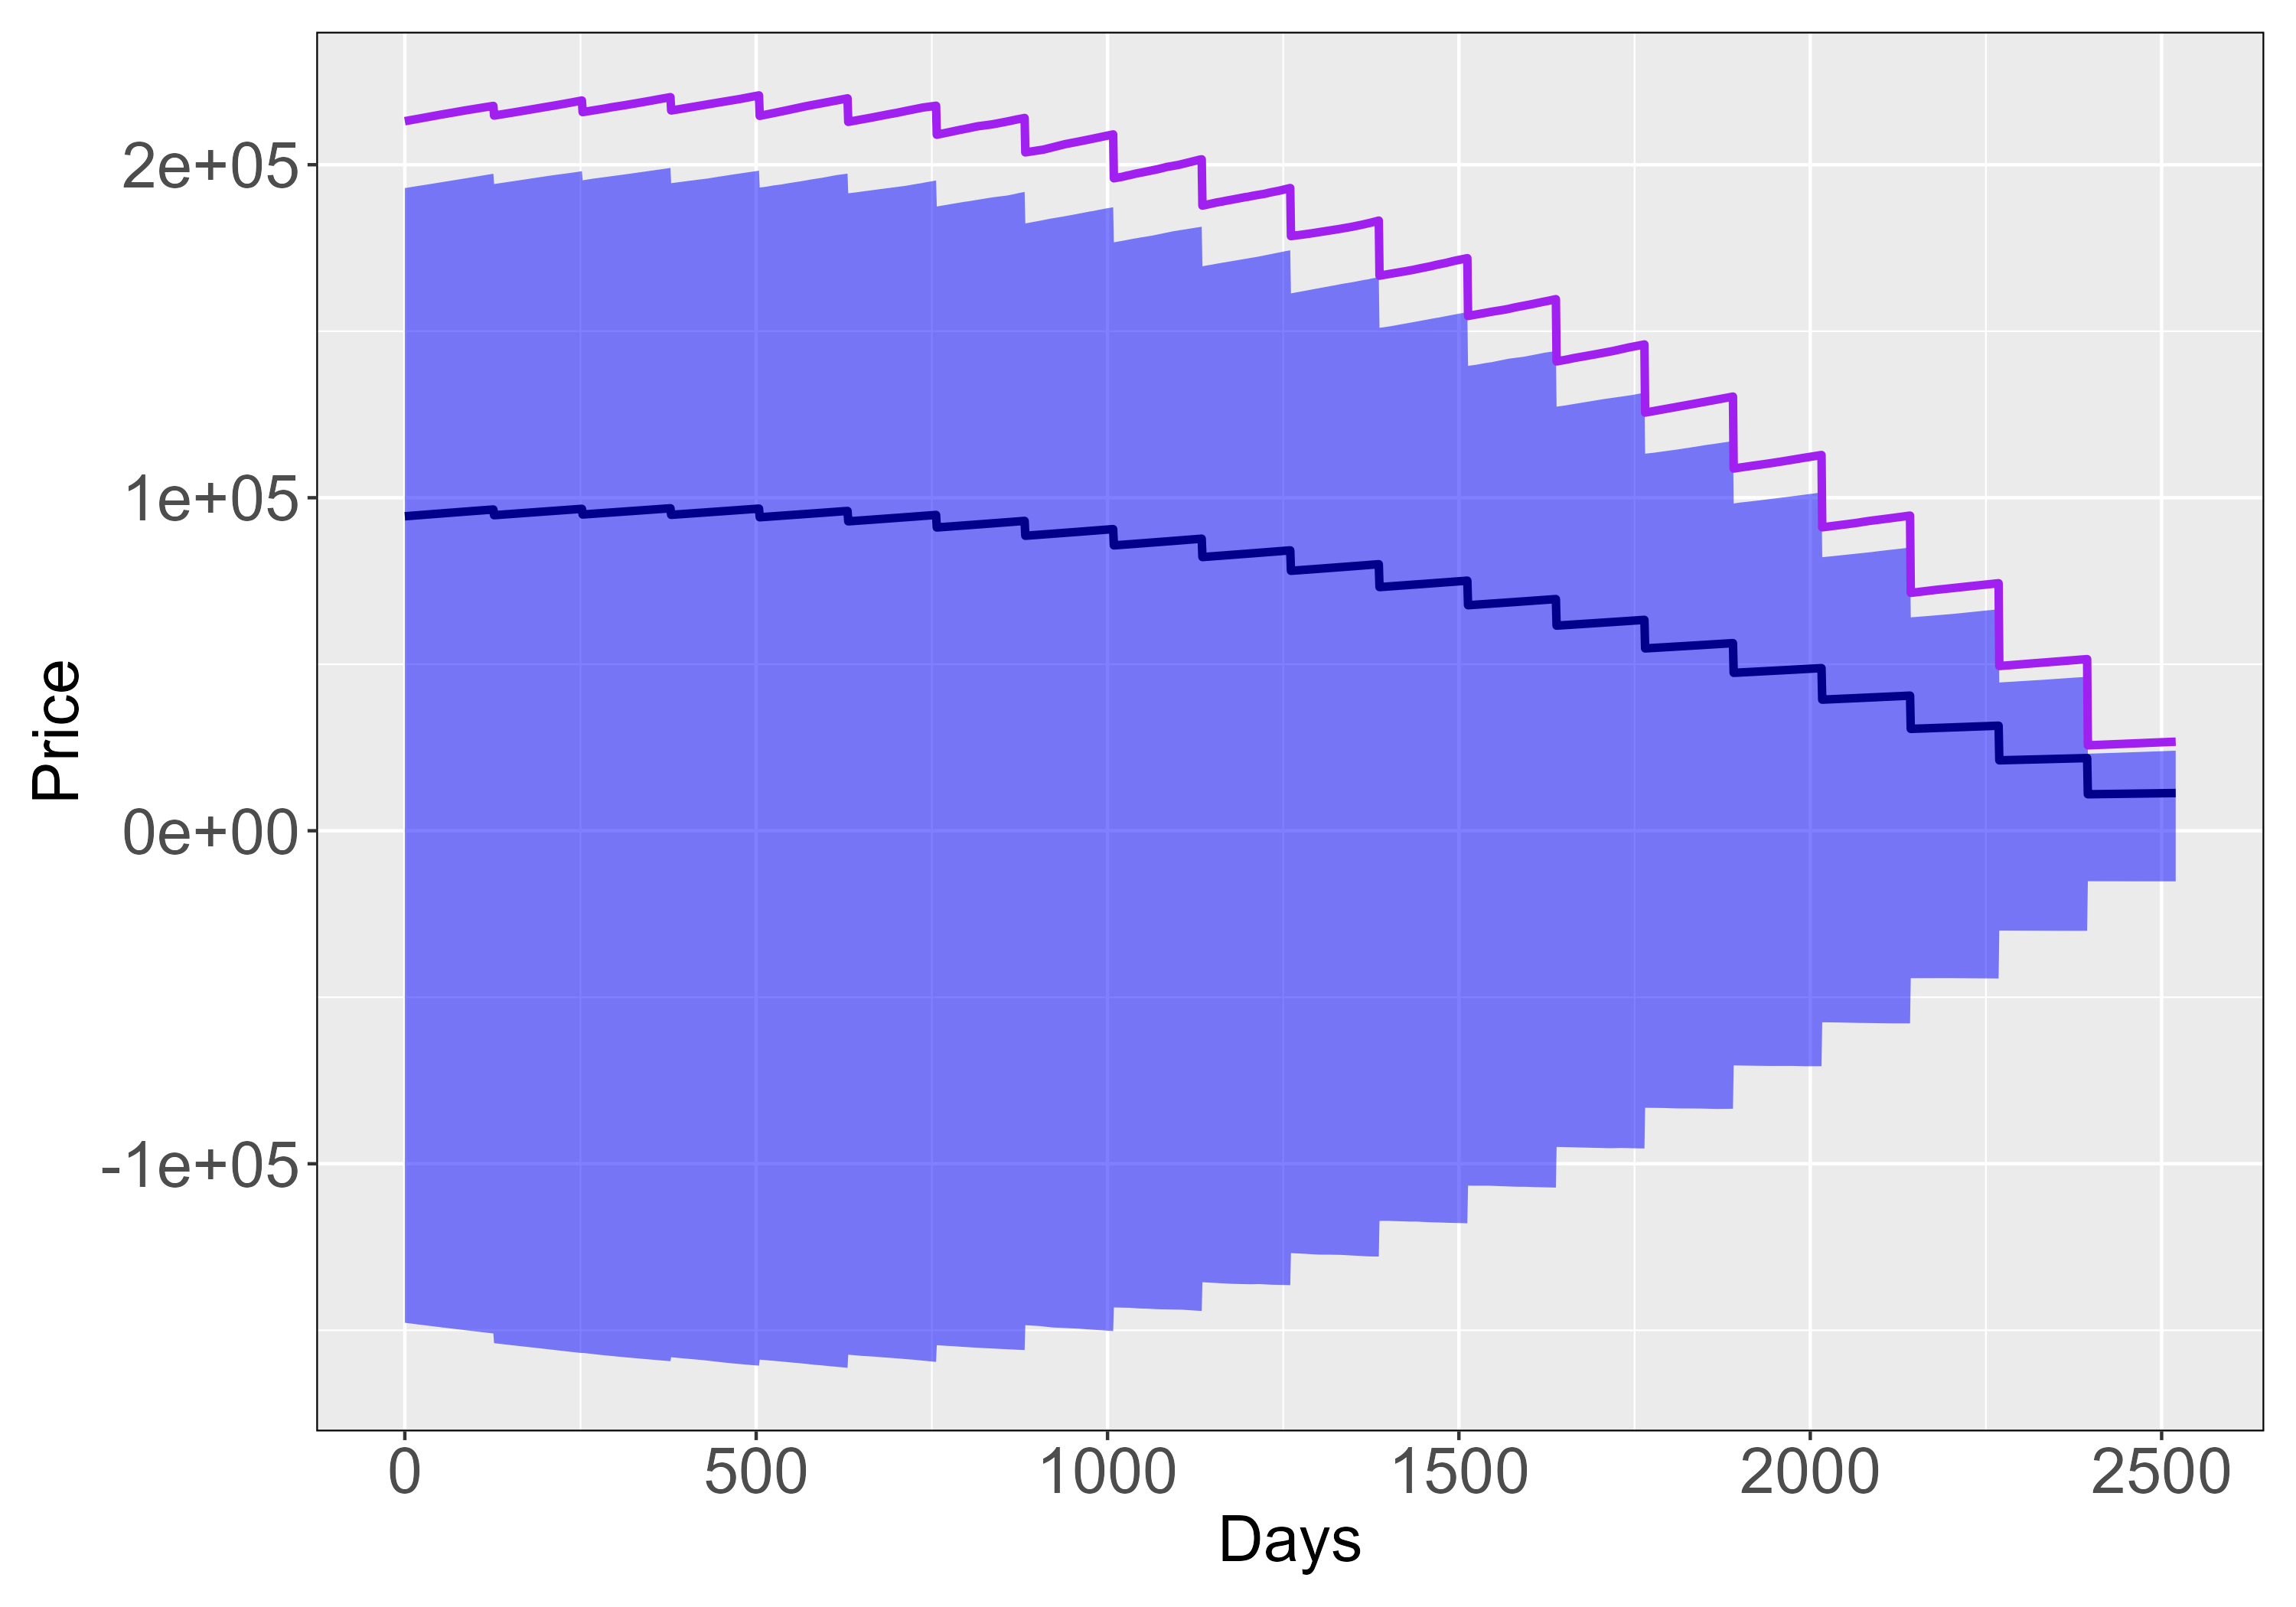
\includegraphics[width=\textwidth]{Figures/Exposure/procedure_2_poly_model_exposure_plot.png}
        \subcaption{Polynomial model using procedure 2.}
        \label{fig:exposure of procedure 2, poly.}
    \end{subfigure}
    \hfill
    \begin{subfigure}{0.49\textwidth}
        \centering
        \captionsetup{justification=centering}
        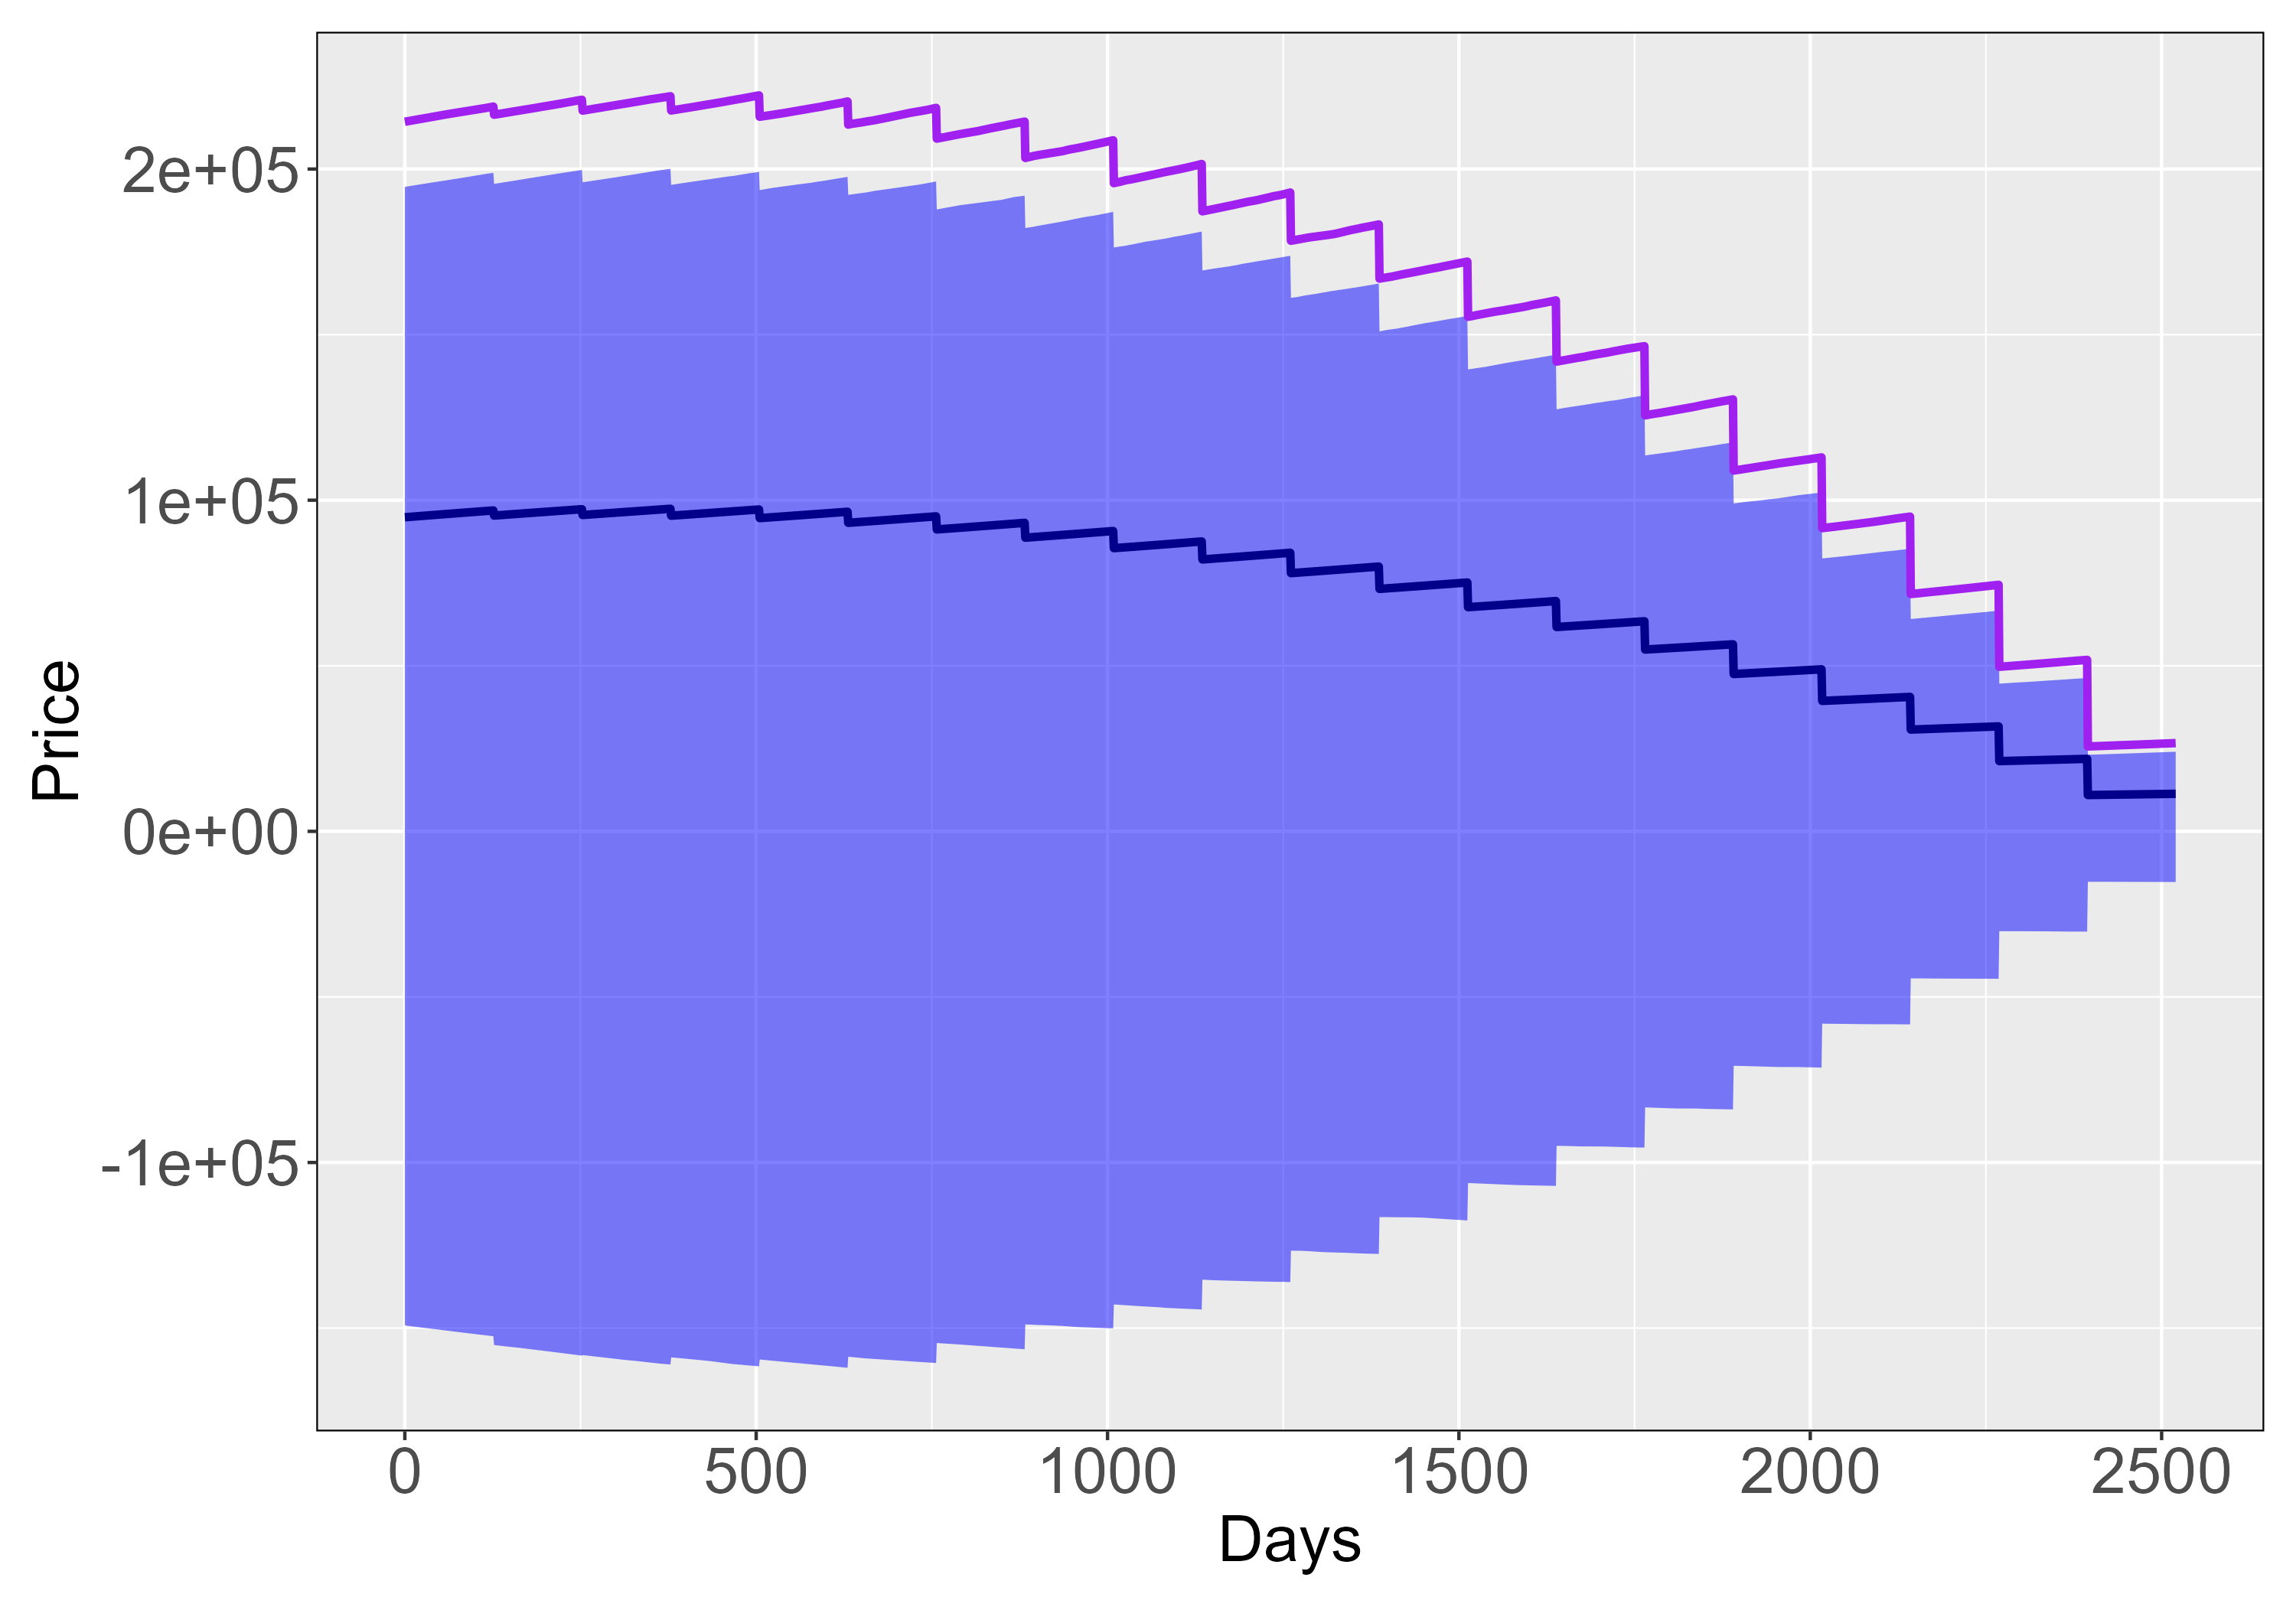
\includegraphics[width=\textwidth]{Figures/Exposure/procedure_2_spline_model_exposure_plot.png}
        \subcaption{Spline model using procedure 2.}
        \label{fig:exposure of procedure 2, spline.}
    \end{subfigure}
    \caption[The exposure from the four different models.]{The exposure from the four different models. The \textbf{dark blue} $\bigl($\textcolor{dark_blue_2}{\textbf{---}}$\bigr)$ line is the expected exposure, the \textbf{purple} $\bigl($\textcolor{purple_}{\textbf{---}}$\bigr)$ line is the Potential future exposure ($95\%$ confidence), and the \textbf{shaded blue} $\bigl($\textcolor{shaded_blue_}{\textbf{---}}$\bigr)$ area is the $95\%$ prediction interval for the price. Again, there is the same result across all models.}
    \label{fig:exposure}
\end{figure}
